% --------------------------------------------------------------------
\section{Introducing the First Law}
% --------------------------------------------------------------------
The First Law of Thermodynamics states that energy is conserved (i.e. neither created nor destroyed).  As we discussed in Section \ref{sec:ch1_energyForms}, we can consider many types of energy (potential, kinetic, chemical, nuclear, and internal), but most of those are either small compared to internal (such as potential and kinetic) or outside the scope of this class (nuclear and chemical).

Energy can be transferred between the system and the surroundings in the form of heat and work, resulting in a change of internal energy of the system. Internal energy change can be considered as a measure of molecular activity associated with change of phase or temperature of the system.

The statement of the first law for closed systems reflects that we are primarily interested in the internal energy ($U$), heat transfer ($Q$), and work ($W$).
\begin{equation} \label{eq:1stLawClosed}
  Q - W = \Delta U
\end{equation}

\begin{figure}[H]
\centering
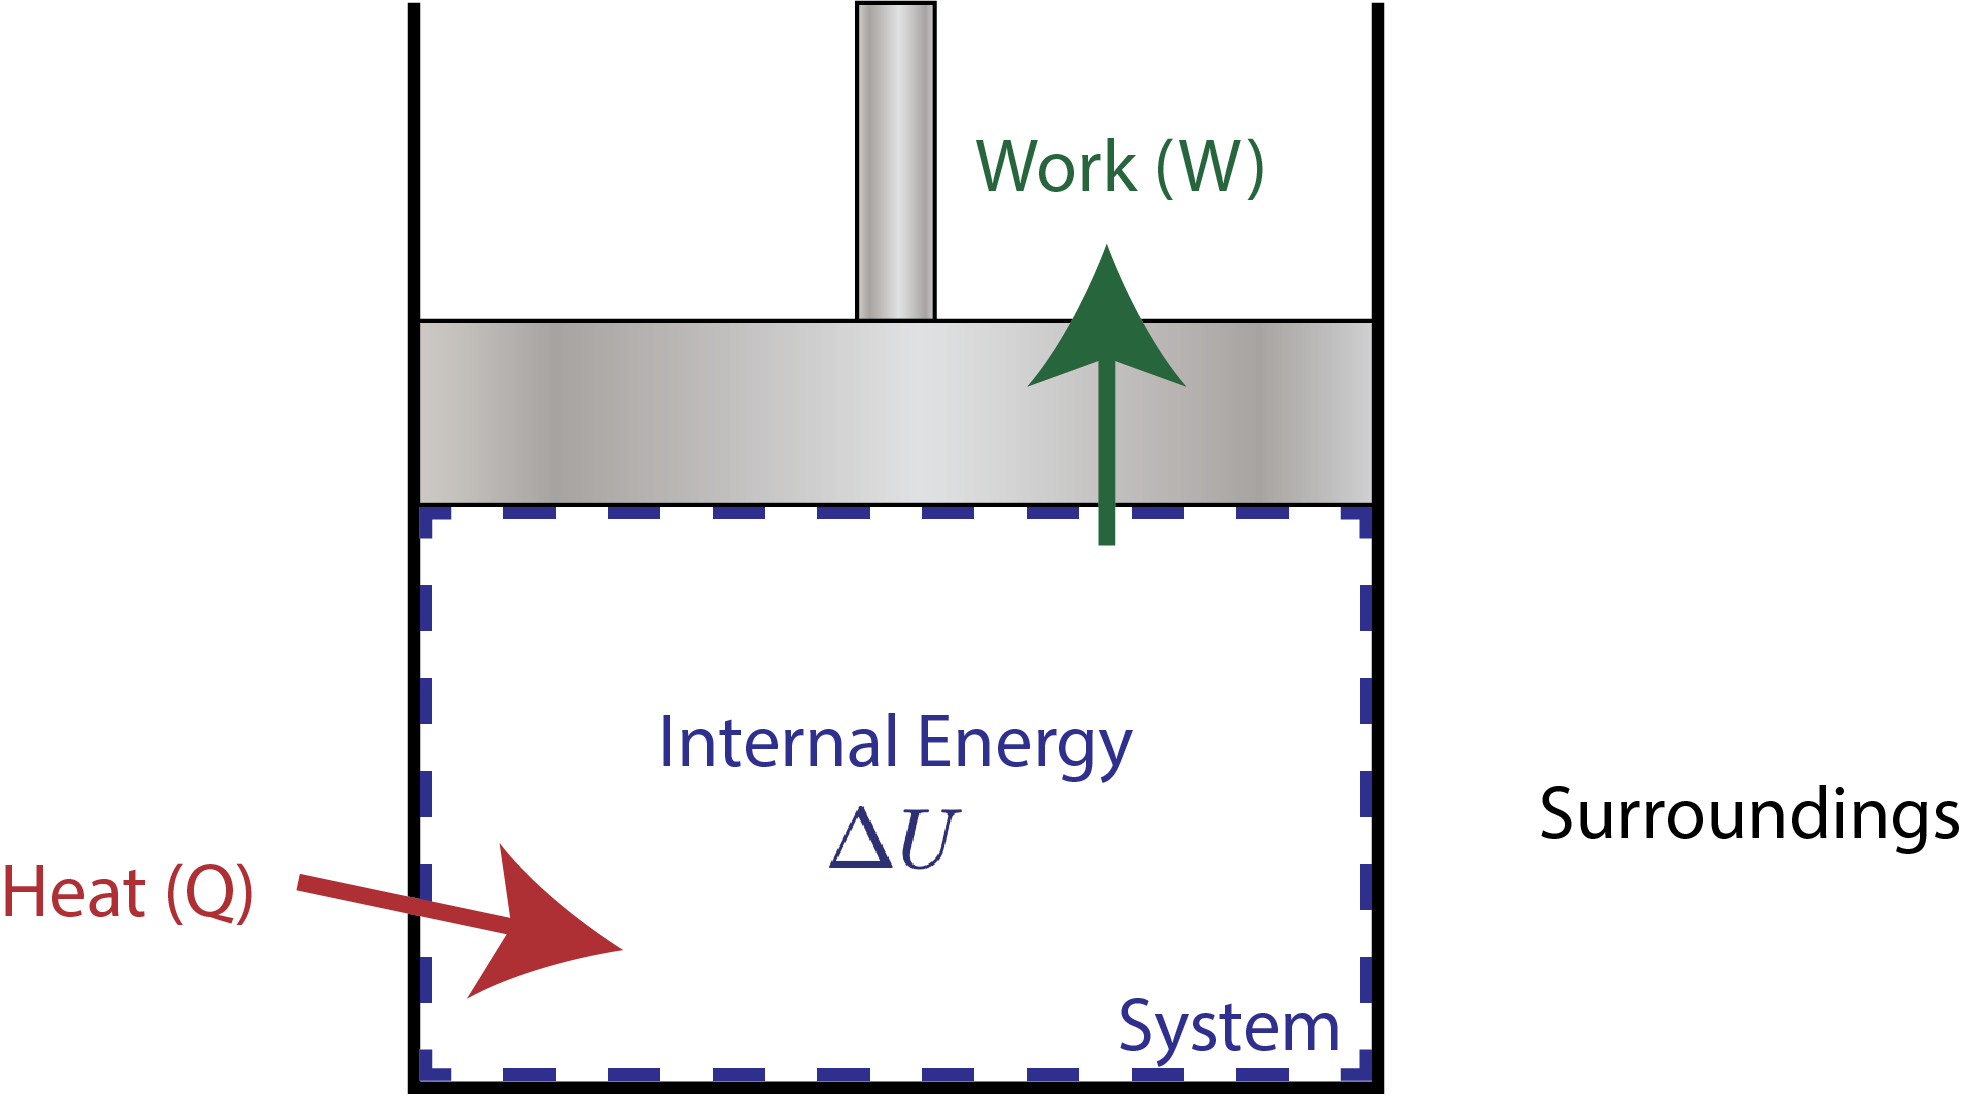
\includegraphics[width=0.5\textwidth]{FirstLaw}
\caption{A closed system with heat transfer and work.}
\label{fig:ch2_energyEquation}
\end{figure}

We can also write the first law by reducing each value to their {\bf mass-specific} counterparts.  Thus, $Q$ becomes $mq$, where $q$ is the mass-specific heat transfer.  $W$ becomes $mw$, where $w$ is the mass-specific work.  $U$ becomes $mu$, where $u$ is the mass-specific internal energy.  As a general rule, a capital variable refers to the extensive value, while the lower-case variable refers to an intensive value (mass is the biggest exception).

After we divide through by mass ($m$), the first law therefore becomes:
\begin{equation*}
  q - w = \Delta u
\end{equation*}

% --------------------------------------------------------------------
\subsection{Heat Transfer ($Q$)}
Energy transferred across the boundary of a system in the form of heat always results from a difference in temperature between the system and its immediate surroundings.  Heat transfer can occur through conduction, convection, or radiation.

{\bf Conduction} is the transfer of heat through direct contact.  When you touch an object hotter than your skin (a stove top, food heated in the oven, etc.), energy moves from the hot object to your colder skin.  The same occurs in reverse when you touch an object colder than your skin.  You typically perceive the movement of heat (not the temperature of the object itself).

{\bf Convection} is the transfer of heat through contact with a moving fluid, such as air or water.  Still air typically feels warmer than moving air (even when both are the same temperature) because the rate of heat transfer is higher.  This leads to the concept of ``wind chill'' in North America, the ``apparent temperature'' in Australia, among others.  These models attempt to show how windy days feel colder than a thermometer reading would indicate.  The \href{https://en.wikipedia.org/wiki/Wind_chill}{wind chill} is calibrated so that the rate of heat transfer is the same between a person walking in the windy weather and on a still day at the wind chill temperature.  The increased heat transfer from convection is also why fans can make a room feel cooler, even if they don't decrease the temperature.

{\bf Radiation} is the transfer of heat through the absorption of light.  Photons are emitted from all substances above absolute zero, and these photons carry energy.  You feel the heat of a fire not through contact with the superheated air, but because the air is hot enough to emit a significant amount of light in the infrared and visible spectrums, which is then absorbed by your skin.  Likewise, you can feel the heat of the sun because the photons are able to travel through the vacuum of space.

The calculation of heat transfer due to temperature differences is left for a later class.  In this book, the quantity of heat transferred during any process will either be specified as part of the problem or evaluated as the unknown of the energy equation.

By convention, {\bf heat is that transferred into the system from the surroundings is considered positive}. Positive heat transfer results in an increase in internal energy of the system.

Heat transfer is {\bf path-dependent} and not a property. It is dependent on the process path between the initial and final states.

Recall in Section \ref{sec:ch1_process} that we introduced some commonly used processes:
\begin{itemize}
\item Isothermal (constant temperature process)
\item Isochoric or isometric (constant volume process)
\item Isobaric (constant pressure process)
\item Adiabatic (no heat flow to or from the system during the process)
\end{itemize}

% --------------------------------------------------------------------
\subsection{Work ($W$)}
%In this course we consider three modes of work transfer across the boundary of a system, as shown in the following diagram:

%\begin{figure}[H]
%\centering
%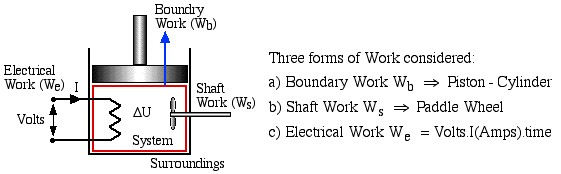
\includegraphics[width=0.75\textwidth]{Work}
%\caption{Description of three types of work.}
%\label{fig:ch2_work}
%\end{figure}

In this course we are primarily concerned with {\bf boundary work} due to compression or expansion of a system in a piston-cylinder device as shown above. In all cases we assume a perfect seal (no mass flow in or out of the system), no loss due to friction, and quasi-equilibrium processes in that for each incremental movement of the piston equilibrium conditions are maintained.

By convention positive work is that done by the system on the surroundings, and negative work is that done by the surroundings on the system.  Since negative work results in an increase in internal energy of the system, this explains the negative sign in Equation \ref{eq:1stLawClosed}.

Boundary work is evaluated by integrating the force $F$ multiplied by the incremental distance moved $dx$ between an initial state (1) to a final state (2). We normally deal with a piston-cylinder device, thus the force can be replaced by the piston area $A$ multiplied by the pressure $p$, allowing us to replace $A\:dx$ by the change in volume $dV$, as follows:

\begin{equation} \label{eq:ch3_work}
  W_{1-2}=\int_1^2F\:dx=\int_1^2pA\:dx=\int_1^2p\:dV=m\int_1^2 p\:dv
\end{equation}

Figure \ref{fig:ch3_pV} provides an example of a piston being compressed.  However, until the process path is specified, it is impossible to know how much work is associated with the compression.  This is seen in the figure as each process has a different area under the curve, which is directly related to the integral in Equation \ref{eq:ch3_work}.  In other words, work done is {\bf path-dependent} and not a property, exactly like heat transfer.

\begin{figure}[H]
\centering
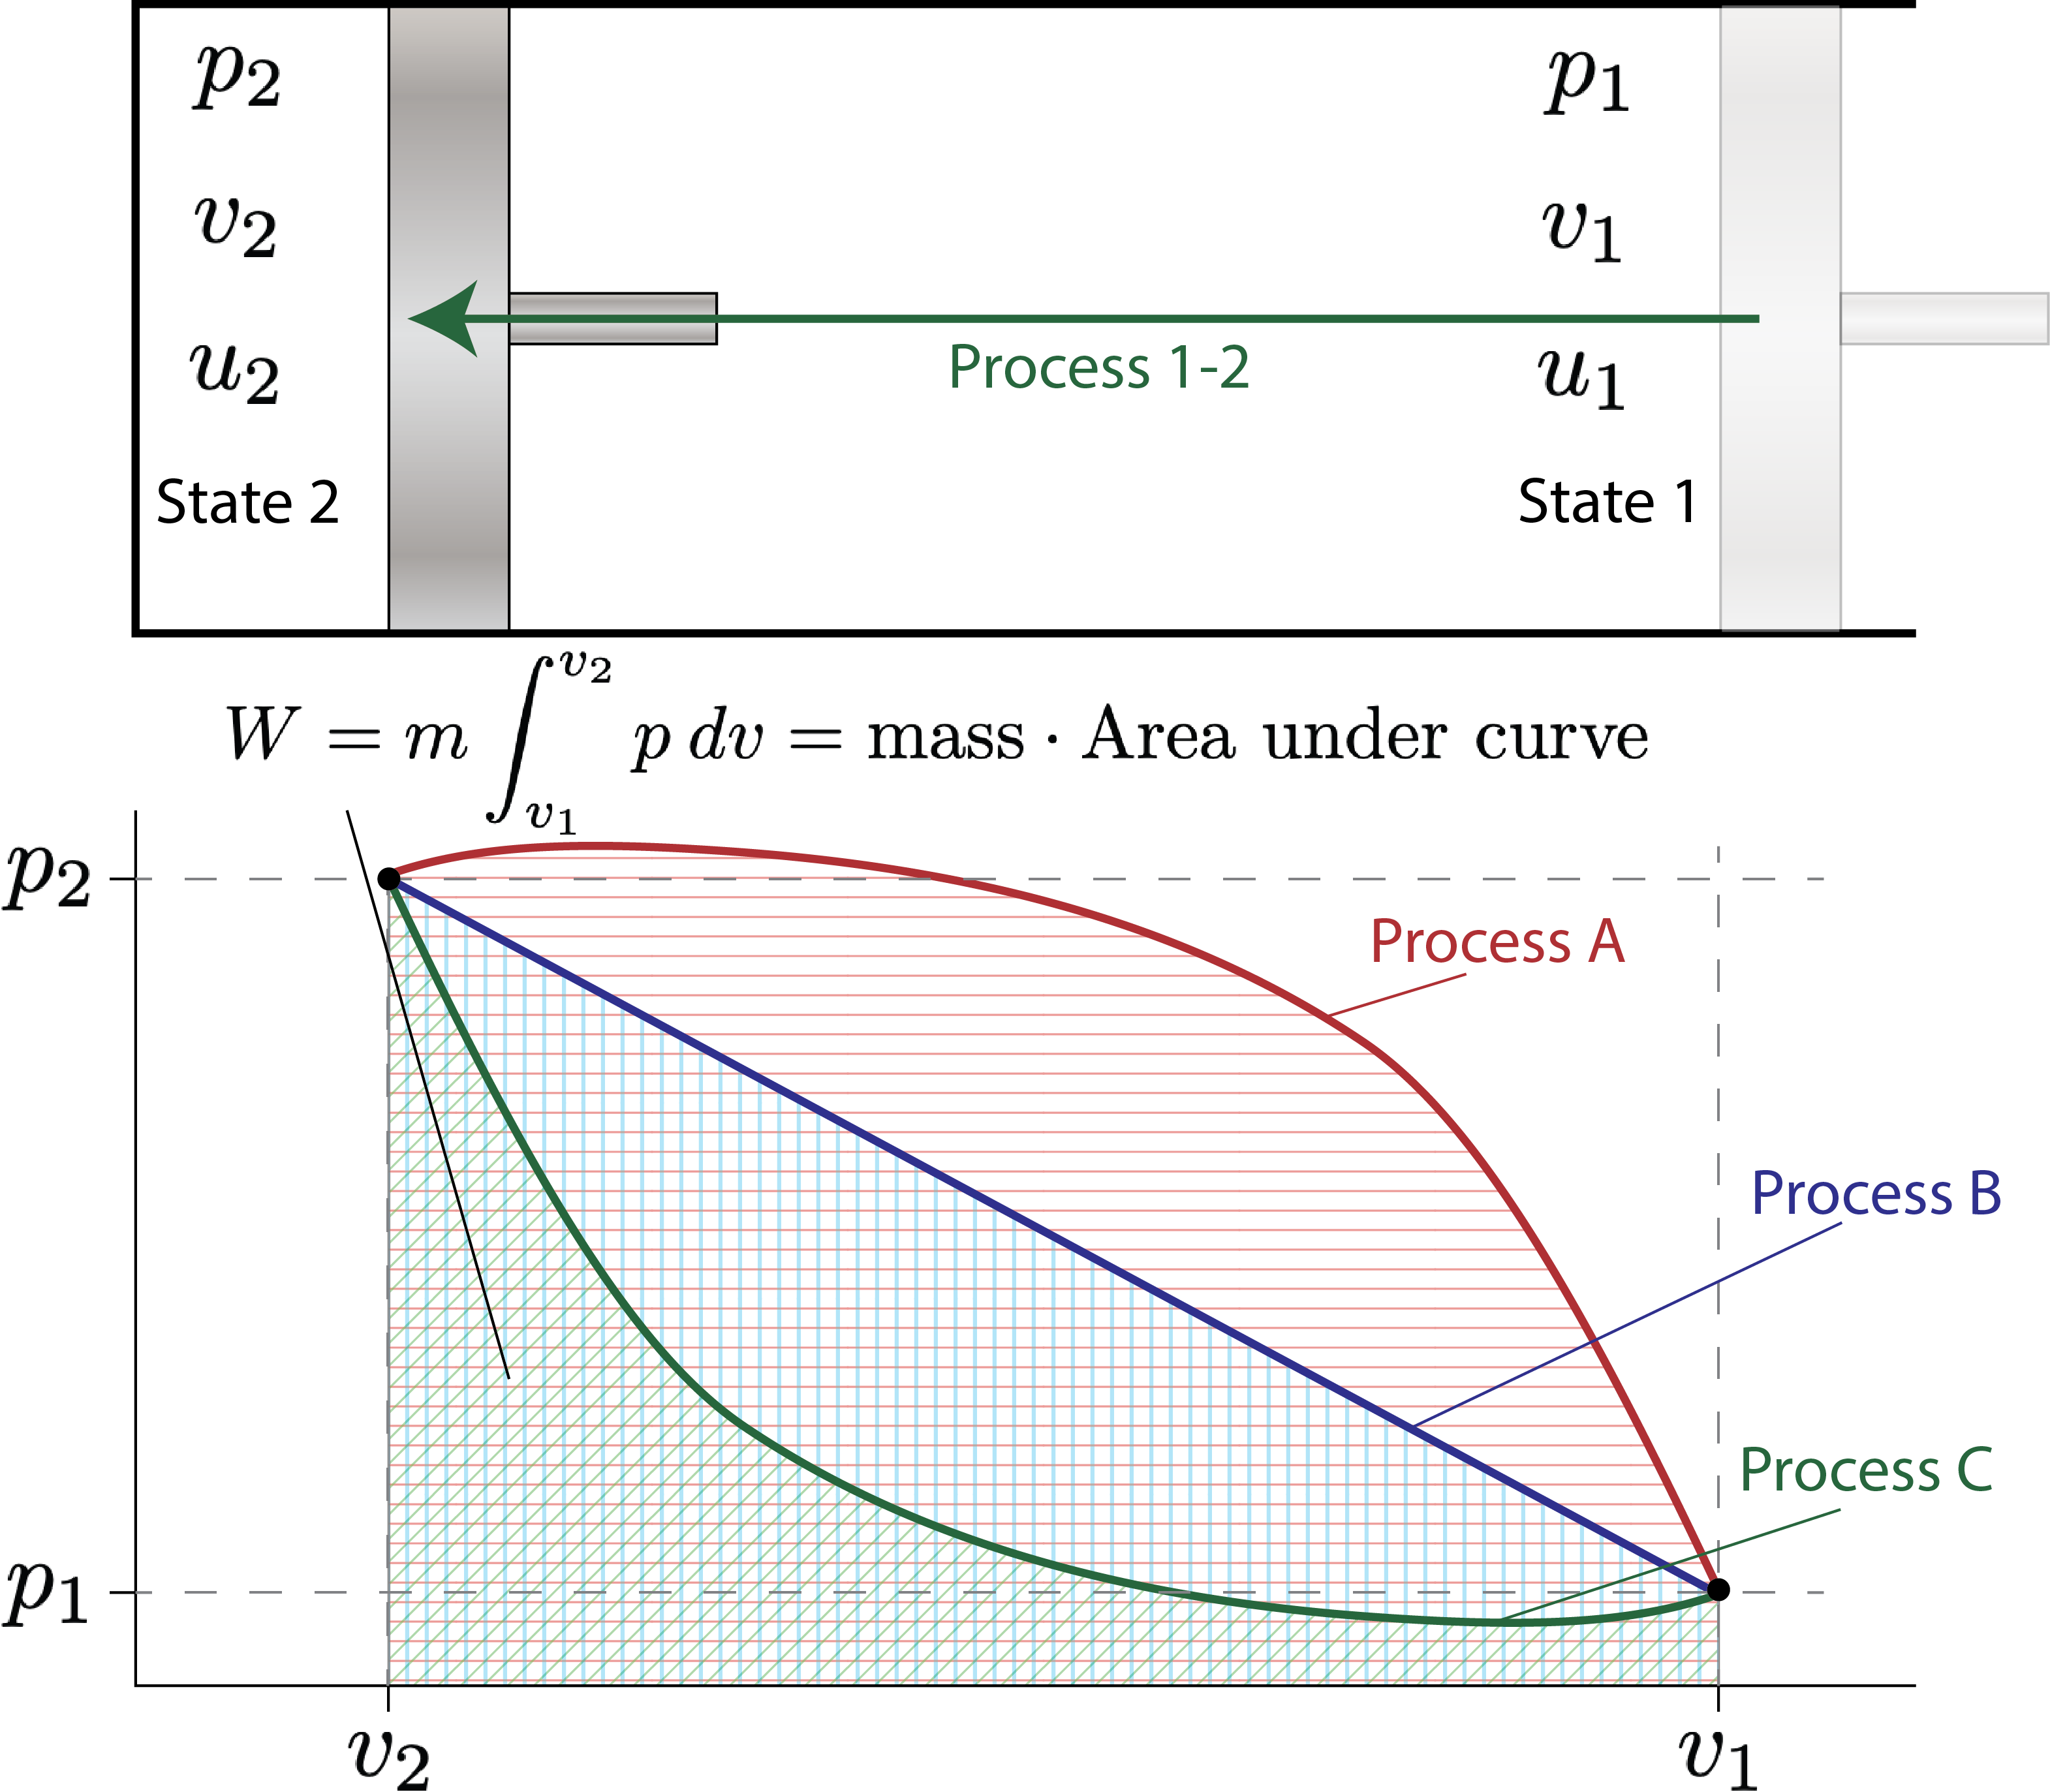
\includegraphics[width=0.75\textwidth]{processWork}
\caption{The state of a piston plotted as air is compressed.  Multiple paths can be taken to connect the same two states.  Processes A, B, and C will have different amounts of work and heat transfer associated with them.}
\label{fig:ch3_pV}
\end{figure}

We note that work done by the system on the surroundings (expansion process) is positive, and that done on the system by the surroundings (compression process) is negative.

Finally, {\bf shaft work} (due to a paddle wheel) and {\bf electrical work} (due to a voltage applied to an electrical resistor or motor driving a paddle wheel) will always be negative (work done on the system). Positive forms of shaft work, such as that due to a turbine, will be considered in Chapter 4 when we discuss open systems.


% --------------------------------------------------------------------
\subsection{Internal Energy ($\Delta U$)}

The third component of Equation \ref{eq:1stLawClosed} is the change of internal energy. Recall from Section \ref{sec:ch1_internalEnergy} that internal energy is closely tied to the temperature of a substance.  In fact, specific internal energy is a property of the system, like temperature and pressure.  From the State Postulate, we can find the internal energy of a state as long as we know at least two other properties.

Often, we prefer to use the mass-specific form of internal energy, which is related to the internal energy in our system as follows:
\begin{equation*}
  u = \frac{U}{m} \quad \rightarrow \quad \Delta u = \frac{\Delta U}{m}
\end{equation*}

Internal energy can be determined from the steam tables in Appendix \ref{ch:appendixSteam} or the R134a tables in Appendix \ref{ch:appendixR134a}.
Heat transfer and work cannot be found from tables because they are not a property of a state, but rather a description of how a process moves between states.

Example \ref{ex:constantPressureRevisited} makes use of the First Law to calculate the heat transfer for a constant pressure process.

\begin{example}[label={ex:constantPressureRevisited}]{Constant Pressure Expansion Revisited}
  Recall Example \ref{ex:ch2constantPressure} in which we presented a constant pressure process. We wish to extend the problem to include the energy interactions of the process, hence we restate it as follows:

  Two kilograms of water at 25°C are placed in a piston cylinder device under 3.2 MPa pressure as shown in the diagram (State (1)). Heat is added to the water at constant pressure until the temperature of the steam reaches 350°C (State (2)).

  Determine the work done by the fluid ($W$) and heat transferred to the fluid ($Q$) during this process.\\

  {\bf Solution Approach}
  We first draw the diagram of the process including all the relevant data as follows:

\begin{center}
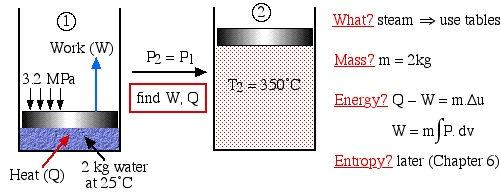
\includegraphics[width=0.75\textwidth]{example3-1}
%\captionof{figure}{}
%\label{fig:ch2_example1}
\end{center}

Notice the four questions to the right of the diagram, which we should always ask before attempting to solve any thermodynamic problem.

\begin{itemize}
  \item {\bf What?} \\
What are we dealing with - liquid? pure fluid, such as steam or refrigerant? ideal gas? In this case it is steam, thus we will use the steam tables to determine the various properties at the various states.

\item {\bf Mass?} \\
Is the mass or volume given? If so we will specify and evaluate the energy equation in kiloJoules rather than specific quantities (kJ/kg).

\item {\bf Energy?}\\
  The energy equation will almost always be our starting point for working through these problems.

\item {\bf Entropy?}\\
What about entropy? Not so fast - wait until Chapter 6.
\end{itemize}
Since work involves the integral of $p\cdot dv$ we find it convenient to sketch the $p$-$v$ diagram of the problem as follows:

\begin{center}
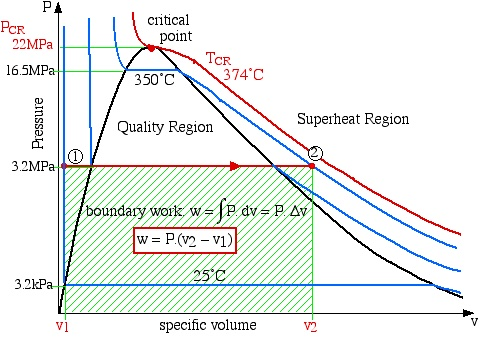
\includegraphics[width=0.75\textwidth]{example3-1_Pv}
%\captionof{figure}{}
%\label{fig:ch2_example1}
\end{center}

Notice on the $p$-$v$ diagram how we determine the specific work done as the area under the process curve. We also notice that in the compressed liquid region the constant temperature line is essentially vertical. Thus all the property values at State (1) (compressed liquid at 25°C) can be determined from the saturated liquid table values at 25°C.

\begin{align*}
  u_1 &= u_{f,\ 25°C}=104.8 \left[\frac{\rm kJ}{\rm kg}\right]\\
  v_1 &= v_{f,\ 25°C}=0.001 \left[\frac{\rm m^3}{\rm kg}\right]
\end{align*}

\begin{center}
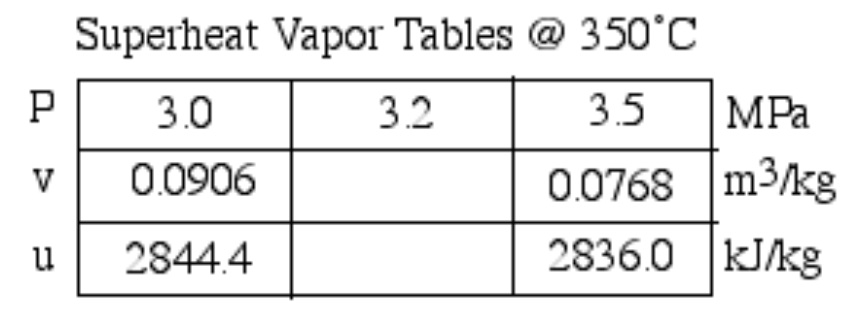
\includegraphics[width=0.5\textwidth]{example3-1_tables}
%\captionof{figure}{}
%\label{fig:ch2_example1}
\end{center}

\begin{align*}
  \frac{\Delta p_A}{\Delta p_b} = \frac{\Delta v_A}{\Delta v_b} &\rightarrow \frac{3.2 - 3.0}{3.5-3.0} = \frac{v_2-0.0906}{0.0768-0.0906} = 0.4\\
  v_2 &= 0.085 \frac{\rm m^3}{\rm kg} \\
  \frac{\Delta p_A}{\Delta p_b} = \frac{\Delta u_A}{\Delta u_b} &\rightarrow \frac{3.2 - 3.0}{3.5-3.0} = \frac{u_2-2844.4}{2836.0-2844.4} = 0.4\\
  u_2 &= 2841 \frac{\rm kJ}{\rm kg}
\end{align*}

Now we use $\Delta v$ to define our work:
\begin{align*}
  W = m \int p dv = m\cdot p \cdot \Delta v = 2.0\ {\rm kg} \cdot 3200\ {\rm kPa} \cdot (0.085 - 0.001)\ \frac{\rm m^3}{\rm kg} \\
  \redbox{W = 538\ {\rm kJ}}
\end{align*}
Then, with work and $\Delta U$, we can find our heat transfer:
\begin{align*}
  \Delta U = Q - W \rightarrow Q = m\cdot (u_2 - u_1) + W \\
  Q = 2.0\ {\rm kg} \cdot (2841 - 104.8)\ \frac{\rm kJ}{\rm kg} + 538\ {\rm kJ} \\
   \redbox{Q = 6010\ {\rm kJ}}
\end{align*}
\end{example}

% --------------------------------------------------------------------
\section{Enthalpy ($h$)- A New Property} \label{sec:ch3_enthalpy}
% --------------------------------------------------------------------

In the case studies that follow we find that one of the major applications of the closed system energy equation is in heat engine processes in which the system is approximated by an ideal gas, thus we will develop relations to determine the internal energy for an ideal gas. We will find also that a new property called {\bf enthalpy} will be useful both for closed systems and in particular for open systems, such as the components of steam power plants or refrigeration systems. Enthalpy is not a fundamental property. Instead, it is a combination of properties and is defined as follows:
\begin{equation}
  h = u + p\cdot v\quad \quad {\rm OR} \quad \quad H = U + p\cdot V
\end{equation}
As with other properties, the lowercase $h$ refers to the mass specific property and is measured in $\frac{\rm kJ}{\rm kg}$, whereas the capital $H$ is an extensive property and is measured in kJ.

Enthalpy shows its use whenever applied to a constant pressure process, such as Example \ref{ex:constantPressureRevisited}.  For these processes, work can be defined as $w = p\cdot \Delta v$, meaning that the energy equation can be written as:
\begin{align*}
  \Delta u &= q - p \Delta v\\
  u_2 - u_1 &= q - p\: (v_2 - v_1)\\
  (u_2 &+ p\: v_2) - (u_1 + p\: v_1) = q \\
  h_2 &- h_1 = q \rightarrow \redbox{q = \Delta h}
\end{align*}

This means that we can look up enthalpy directly to find heat transfer {\bf for constant pressure processes}.

% --------------------------------------------------------------------
\section{Specific Heats} \label{sec:specificHeats}
% --------------------------------------------------------------------

For solids and liquids, we can define a relatively simple equation:
\begin{equation} \label{eq:calorimetry}
  Q = mc\Delta T\quad\quad {\rm OR} \quad\quad q=c\Delta T
\end{equation}
The variable $c$ is called the {\bf specific heat}, and is a relationship between the amount of heat added to a material and the temperature increase we expect.  This is often discussed in chemistry alongside devices known as calorimeters.

% --------------------------------------------------------------------
\subsection{Constant Volume}
In this section, we will expand the concept of specific heat to gases.  To start, let's consider $u$ as a function of $T$ and $v$:
\begin{equation*}
  u = u(T, v)
\end{equation*}

Using the concept of the {\bf total differential} from Calculus, we can write:
\begin{equation*}
  du = \frac{\partial u}{\partial T}dT + \frac{\partial u}{\partial v}dv
\end{equation*}

Since a partial derivative only considers change from a single variable, and we assumed that $u$ was a function only of $T$ and $v$, $\partial u / \partial T$ is the same as saying ``the change of $u$ with respect to $T$ when $v$ is constant''.

However, we could have written $u$ as a function of any two independent properties, so to specify exactly which one, we'll add the property that stays constant as a subscript:
\begin{equation*}
  \frac{\partial u}{\partial T} = \left[\frac{d u}{d T}\right]_v
\end{equation*}

Writing $du$ again, we get:
\begin{equation}\label{eq:du_Tv}
  du = \left[\frac{d u}{d T}\right]_v dT + \left[\frac{d u}{d v}\right]_T dv
\end{equation}

Now, let's write the energy equation in differential form.  Recall that $w = p \Delta v$, which can be written in differential form as $\delta w = p\: dv$.
\begin{equation}\label{eq:differentialEnergy}
  \delta q - \delta w = du \quad \rightarrow \quad \delta q - p\: dv = du
\end{equation}

We used $\delta q$ and $\delta w$ because $q$ and $w$ are not properties, and therefore not integrable in the same way as $v$ and $u$.

Combining Equations \ref{eq:du_Tv} and \ref{eq:differentialEnergy}, we get:
\begin{equation*}
  \delta q = \left[\frac{d u}{d T}\right]_v dT + \left(\left[\frac{d u}{d v}\right]_T + p \right) dv
\end{equation*}

All of this leads to a huge simplification for constant-volume processes.  If $dv = 0$, we get the following:
\begin{equation} \label{eq:cv1}
  \delta q = \left[\frac{d u}{d T}\right]_v dT
\end{equation}

Equation \ref{eq:cv1} is simply the differential form of Equation \ref{eq:calorimetry}!  In fact, $\left[\frac{d u}{d T}\right]_v$ is simply the {\bf constant volume specific heat}, $c_v$.

% --------------------------------------------------------------------
\subsection{Constant Pressure}

Now we could have started this discussion by defining $h$ as a function of $T$ and $p$.
\begin{equation*}
  h = h(T, p)
\end{equation*}
That would result in:
\begin{equation}\label{eq:dh_Tp}
  dh = \left[\frac{d h}{d T}\right]_p dT + \left[\frac{d h}{d p}\right]_T dp
\end{equation}
We know that the second half will eventually fall off when we think about constant pressure systems.

Let's expand $dh$, using our definition of $h=u + pv$.  In order to do so, we need to remember the Product Rule from Calculus: $(fg)' = f'g + g'f$
\begin{align}
  \nonumber dh &= d(u + pv) = du + d(pv) \\
  \label{eq:dhExpanded} dh &= du + p\: dv + v\: dp
\end{align}

Now, we can replace $du$ with $\delta q - p\: dv$, based on Equation \ref{eq:differentialEnergy}:
\begin{align*}
  dh &= (\delta q - p\: dv) + p\: dv + v\: dp \\
  dh &= \delta q + v\: dp
\end{align*}

Next, we plug our result into Equation \ref{eq:dh_Tp}:
\begin{align*}
  \delta q + v\: dp &= \left[\frac{d h}{d T}\right]_p dT + \left[\frac{d h}{d p}\right]_T dp \\
  \delta q &= \left[\frac{d h}{d T}\right]_p dT + \left(\left[\frac{d h}{d p}\right]_T  - v \right)dp
\end{align*}

Finally, we implement the constant pressure assumption, which sets $dp=0$:
\begin{equation} \label{eq:cp1}
  \delta q = \left[\frac{d h}{d T}\right]_p dT
\end{equation}

Again, with Equation \ref{eq:cp1}, we can state that $\left[\frac{d h}{d T}\right]_p$ is the {\bf constant pressure specific heat}, $c_p$.

% --------------------------------------------------------------------
\subsection{Ideal Gases}
Now, consider $u$ and $h$ for ideal gases.  We state without proof that for an ideal gas, internal energy depends on temperature alone.  In other words, $u$ and $c_v$ are purely functions of temperature.

With $u=u(T)$ and $pv = RT$, we can write:
\begin{equation*}
  h = u + pv = u(T) + RT
\end{equation*}

This means that $h$ is also only a function of temperature!  In fact, by evaluating $d h/d T$, we can say:
\begin{equation} \label{eq:ch3_cpcvR}
  \frac{d h}{d T} = \frac{d u}{d T} + R \quad\rightarrow\quad c_p = c_v + R
\end{equation}

Because both $c_p$ and $c_v$ are only functions of temperature, we can drastically reduce the amount of information needed for the tables.  A single table (Appendix \ref{sec:idealGasAir}) is sufficient for all ideal gas properties. In fact, we can even assume a constant specific heat and retain good accuracy, as long as the specific heat is evaluate at the average temperature, $T_{avg}$.

\begin{equation}
  \Delta u = c_v(T_{avg})\cdot \Delta T  \quad \quad\quad \Delta h = c_p(T_{avg})\cdot \Delta T
\end{equation}

\begin{example}{Ideal Gas $u$ and $h$}
  Air at 300 K undergoes a process in which heat is added at constant pressure.  Consider processes that end at 900 K, 1200 K, and 1500 K.
  Determine the heat added using a) $c_p(T_{avg})$ and b) the enthalpies given in the table.

  {\bf Solution Approach}
  Since the process occurs at constant pressure, we know that the heat added is simply the difference in enthalpy:
  \begin{equation*}
    Q = h_2 - h_1
  \end{equation*}

  If we assume constant specific heat, we can also say that:
  \begin{equation*}
    Q = c_p \left(T_2 - T_1\right)
  \end{equation*}

  \begin{enumerate}[a)]
  \item We first need to find the $c_p$ at the average process temperatures.
    \begin{center}
      \begin{tabular}{ccc}
        $T_2$ & $T_{avg}$ & $c_p(T_{avg})$ \\ \hline
        900 K & 600 K & 1.0509 kJ/kgK \\
        1200 K & 750 K & 1.0866 kJ/kgK \\
        1500 K & 900 K & 1.1208 kJ/kgK
      \end{tabular}
    \end{center}
    Note that we needed to use linear interpolation in order to find the $c_p$ at 750 K.

    With the $c_p$ values in hand, we can find $Q$:
    \begin{center}
      \begin{tabular}{cccc}
        $T_2$ & $\Delta T$ & $c_p(T_{avg})$ & $Q$\\ \hline
        900 K & 600 K & 1.0509 kJ/kgK & 630.54 kJ/kg\\
        1200 K & 900 K & 1.0866 kJ/kgK & 977.94 kJ/kg\\
        1500 K & 1200 K & 1.1208 kJ/kgK & 1344.96 kJ/kg
      \end{tabular}
    \end{center}
    The rightmost column above is our desired result.
  \item The second method requires us to find the enthalpies directly.  The enthalpy of air at 300 K is 426.53 kJ/kg.  The enthalpies at the end of the process, along with the resulting heat transfers, are given below:
    \begin{center}
      \begin{tabular}{ccc}
        $T_2$ & $h_2$ & $Q$ \\ \hline
        900 K & 1059.36 kJ/kg & 632.83 kJ/kg \\
        1200 K & 1404.14 kJ/kg & 977.61 kJ/kg \\
        1500 K & 1762.29 kJ/kg & 1335.76 kJ/kg
      \end{tabular}
    \end{center}
    Again, the rightmost column is our desired result.
  \end{enumerate}
  Comparing the two methods, we can find the percent error through the formula:
  \begin{equation*}
    err = \frac{Q_a-Q_b}{Q_b} \times 100 \%
  \end{equation*}
  Finally, we see the errors below:
  \begin{center}
      \begin{tabular}{cc}
        $T_2$ & Error \\ \hline
        900 K & -0.36\%\\
        1200 K & 0.034\% \\
        1500 K & 0.69\%
      \end{tabular}
  \end{center}
  In all three cases, we see less than 1\% error, meaning that the average $c_p$ method is very accurate for air.
\end{example}
\newpage
% --------------------------------------------------------------------
\section{Stirling Cycle Engine} \label{sec:ch3_stirling}
% --------------------------------------------------------------------
\label{sec:idealStirling}
Conceptually, the Stirling engine, invented by Robert Stirling, is the simplest of all heat engines. It has no valves, and includes an externally heated space and an externally cooled space. 

In its original form the working gas (typically air or helium) is sealed within a single cylinder by the piston and shuttled between the hot and cold spaces by a displacer, as seen in Figure \ref{fig:ch3_stirlingAll}. The linkage driving the piston and displacer will move them such that the gas will compress while it is mainly in the cool compression space and expand while in the hot expansion space. This is clearly illustrated in \href{https://en.wikipedia.org/wiki/Stirling_engine#/media/File:Stirling_Animation.gif}{this animation} which was produced by Richard Wheeler (Zephyris) of Wikipedia.

\begin{figure}[H]
\centering
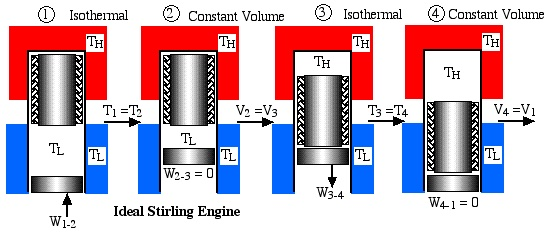
\includegraphics[width=0.75\textwidth]{StirlingEngine}
\caption{The states of the Stirling engine cycle.}
\label{fig:ch3_stirlingAll}
\end{figure}
Refer also to the \href{http://animatedengines.com/stirling.html}{animation produced by Matt Keveney} in his Stirling engine animation website. Since the gas is at a higher temperature, and therefore pressure, during its expansion than during its compression, more power is produced during expansion than is reabsorbed during compression, and this net excess power is the useful output of the engine. Note that there are no valves or intermittent combustion, which is the major source of noise in an internal combustion engine. The same working gas is used over and over again, making the Stirling engine a sealed, closed cycle system. All that is added to the system is steady high temperature heat, and all that is removed from the system is low temperature (waste) heat and mechanical power.

Please note that the following analysis of Stirling cycle engines is ideal, and is intended only as an example of First Law Analysis of closed systems. In the real world we cannot expect actual machines to perform any better than 40 - 50\% of the ideal machine.
%The analysis of actual Stirling cycle machines is extremely complex and requires sophisticated computer analysis (see for example the web learning resource on: \href{https://www.ohio.edu/mechanical/stirling/index.html}{Stirling Cycle Machine Analysis}).

The four states of the Stirling engine are summarized in Figure \ref{fig:ch3_stirlingAll} and Figure \ref{fig:ch3_stirlingDiagram}.  Note specifically the motion of both the piston and the displacer.  The movement of the piston correlates to the compression or expansion of the fluid, while the action of the displacer is to move the fluid between the hot and cold regions, thereby heating or cooling the fluid.

In essence, the ideal Stirling engine undergoes four distinct processes, each of which can be analyzed separately: isothermal compression at $T_C$, constant volume heating at $v_{min}$, isothermal expansion at $T_H$, and constant volume cooling (or heat rejection) at $v_{max}$.

\begin{figure}[H]
\centering
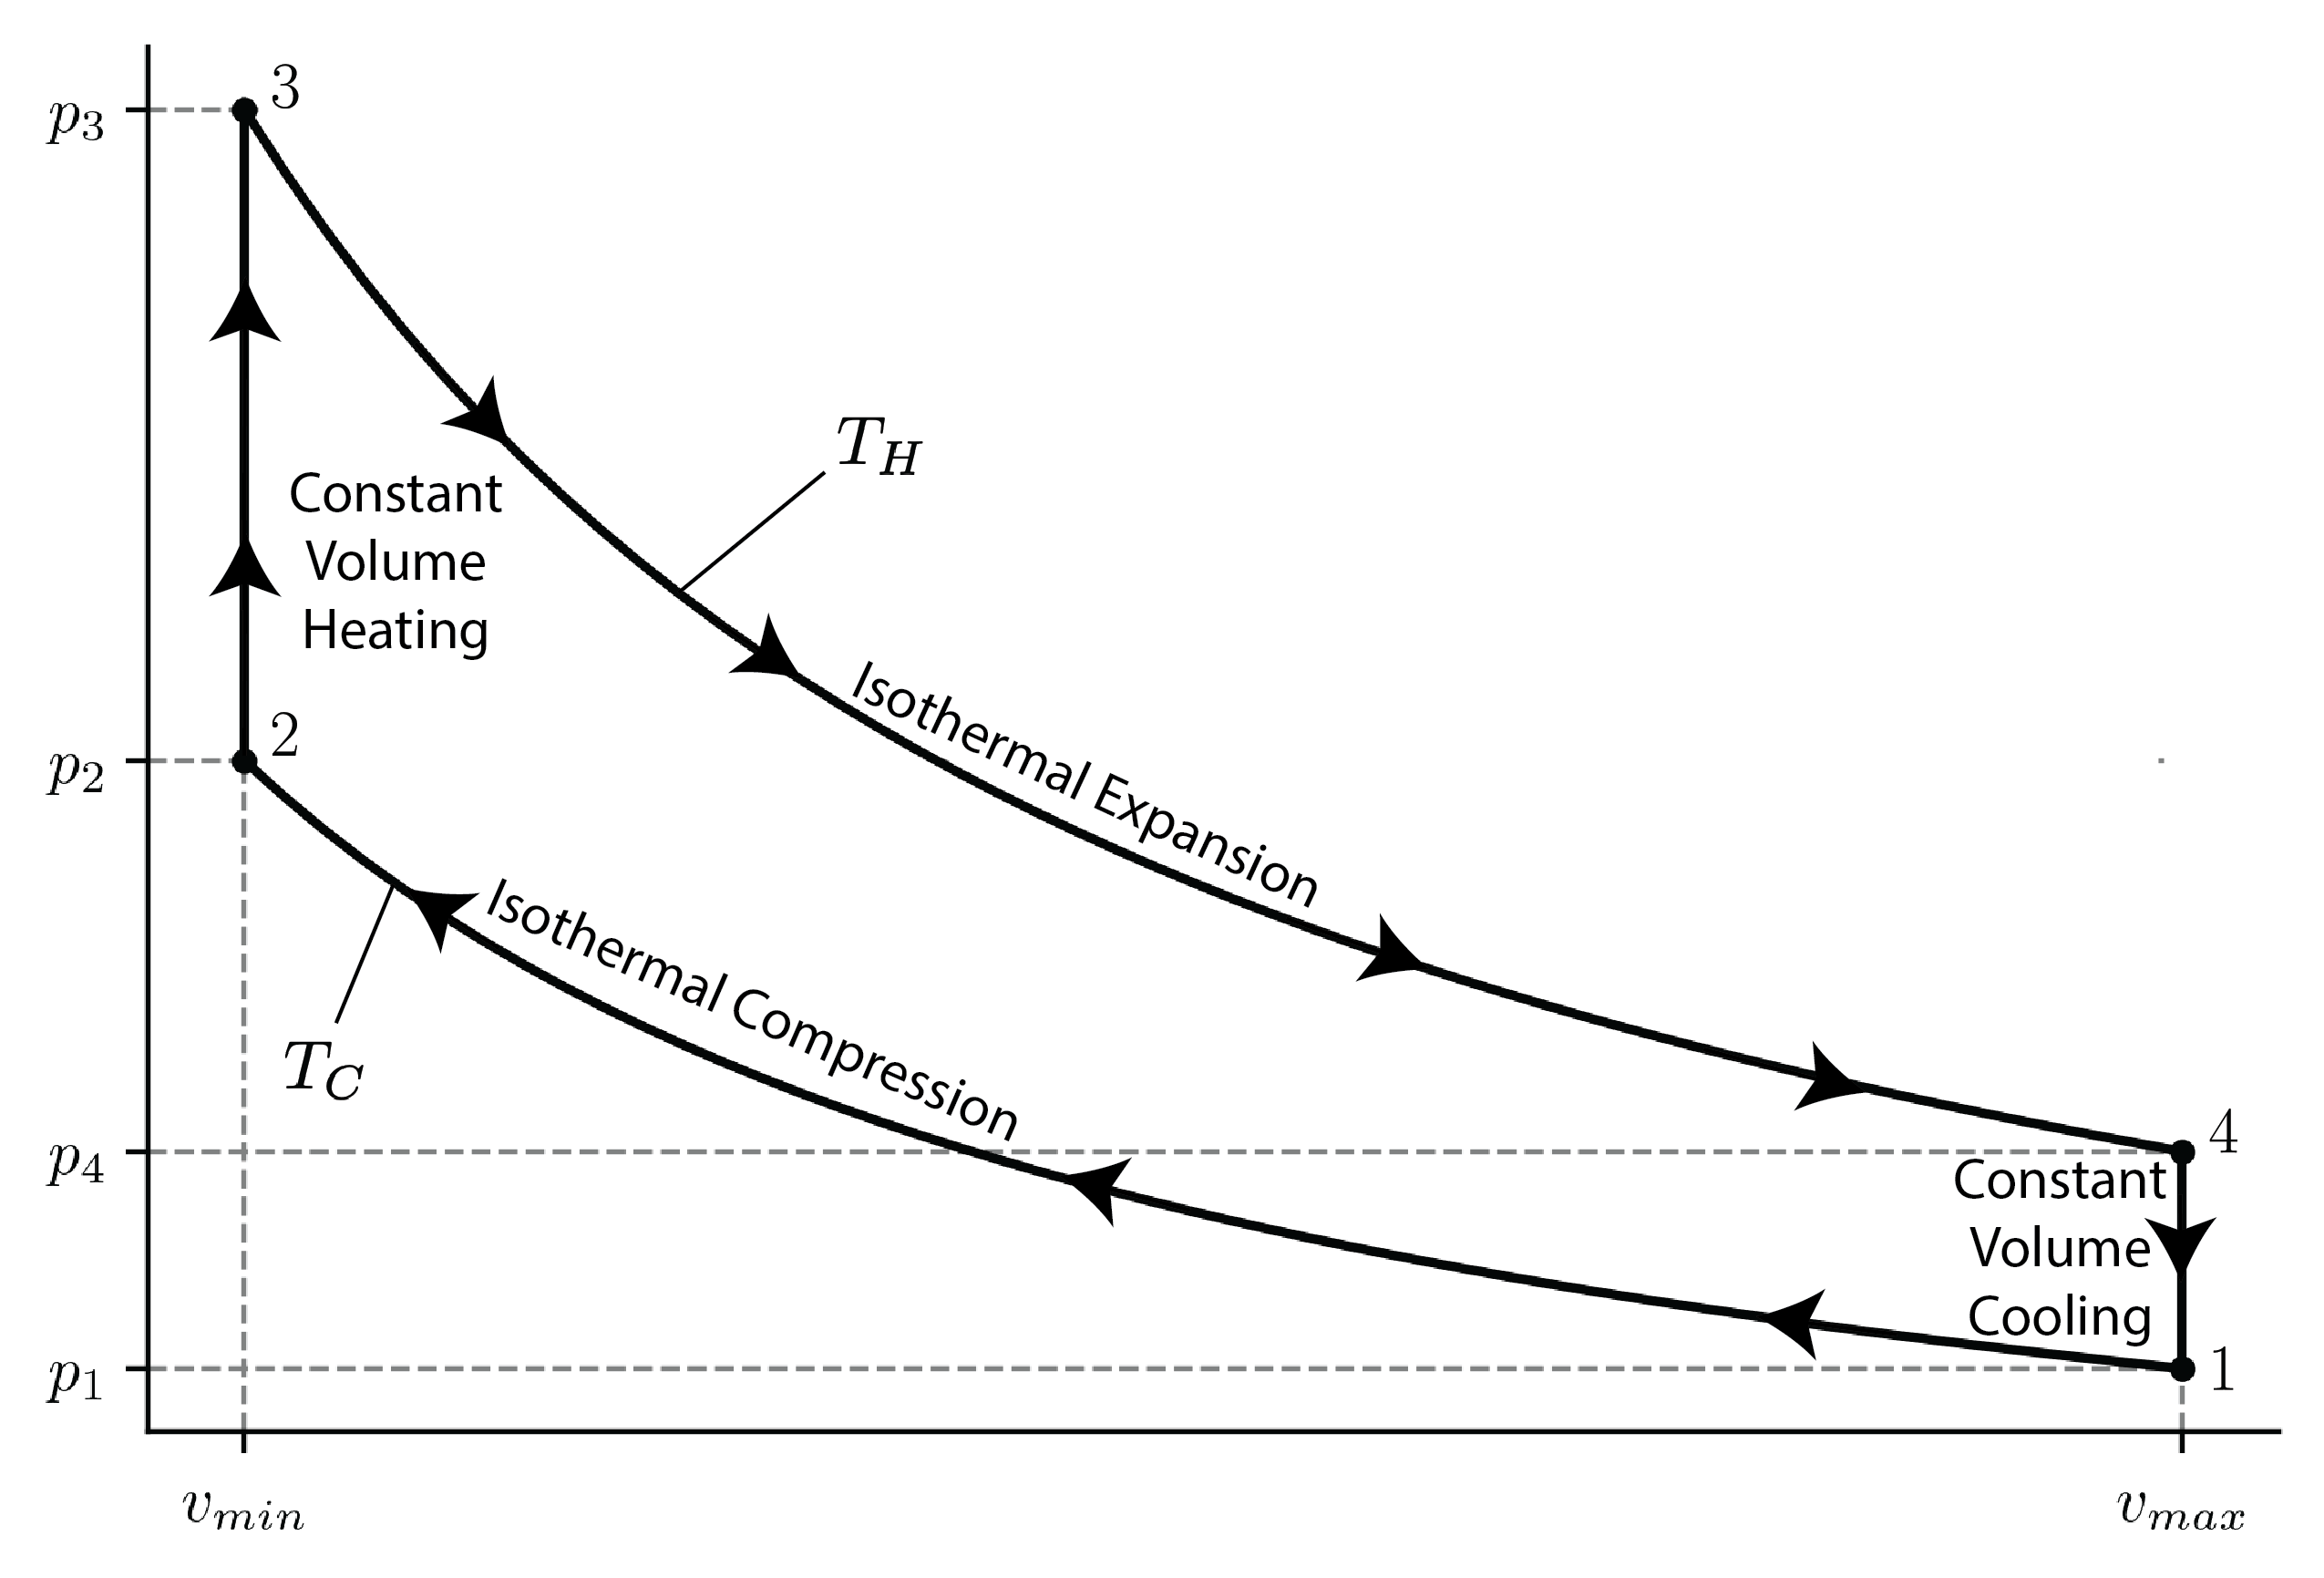
\includegraphics[width=0.75\textwidth]{StirlingDiagram}
\caption{The states of the Stirling engine cycle.}
\label{fig:ch3_stirlingDiagram}
\end{figure}

% --------------------------------------------------------------------
\subsection{Process 1$\rightarrow$2 -- Isothermal Compression}
We start our analysis at State 1, which is the coolest and least compressed point of the cycle.

\begin{figure}[H]
\centering
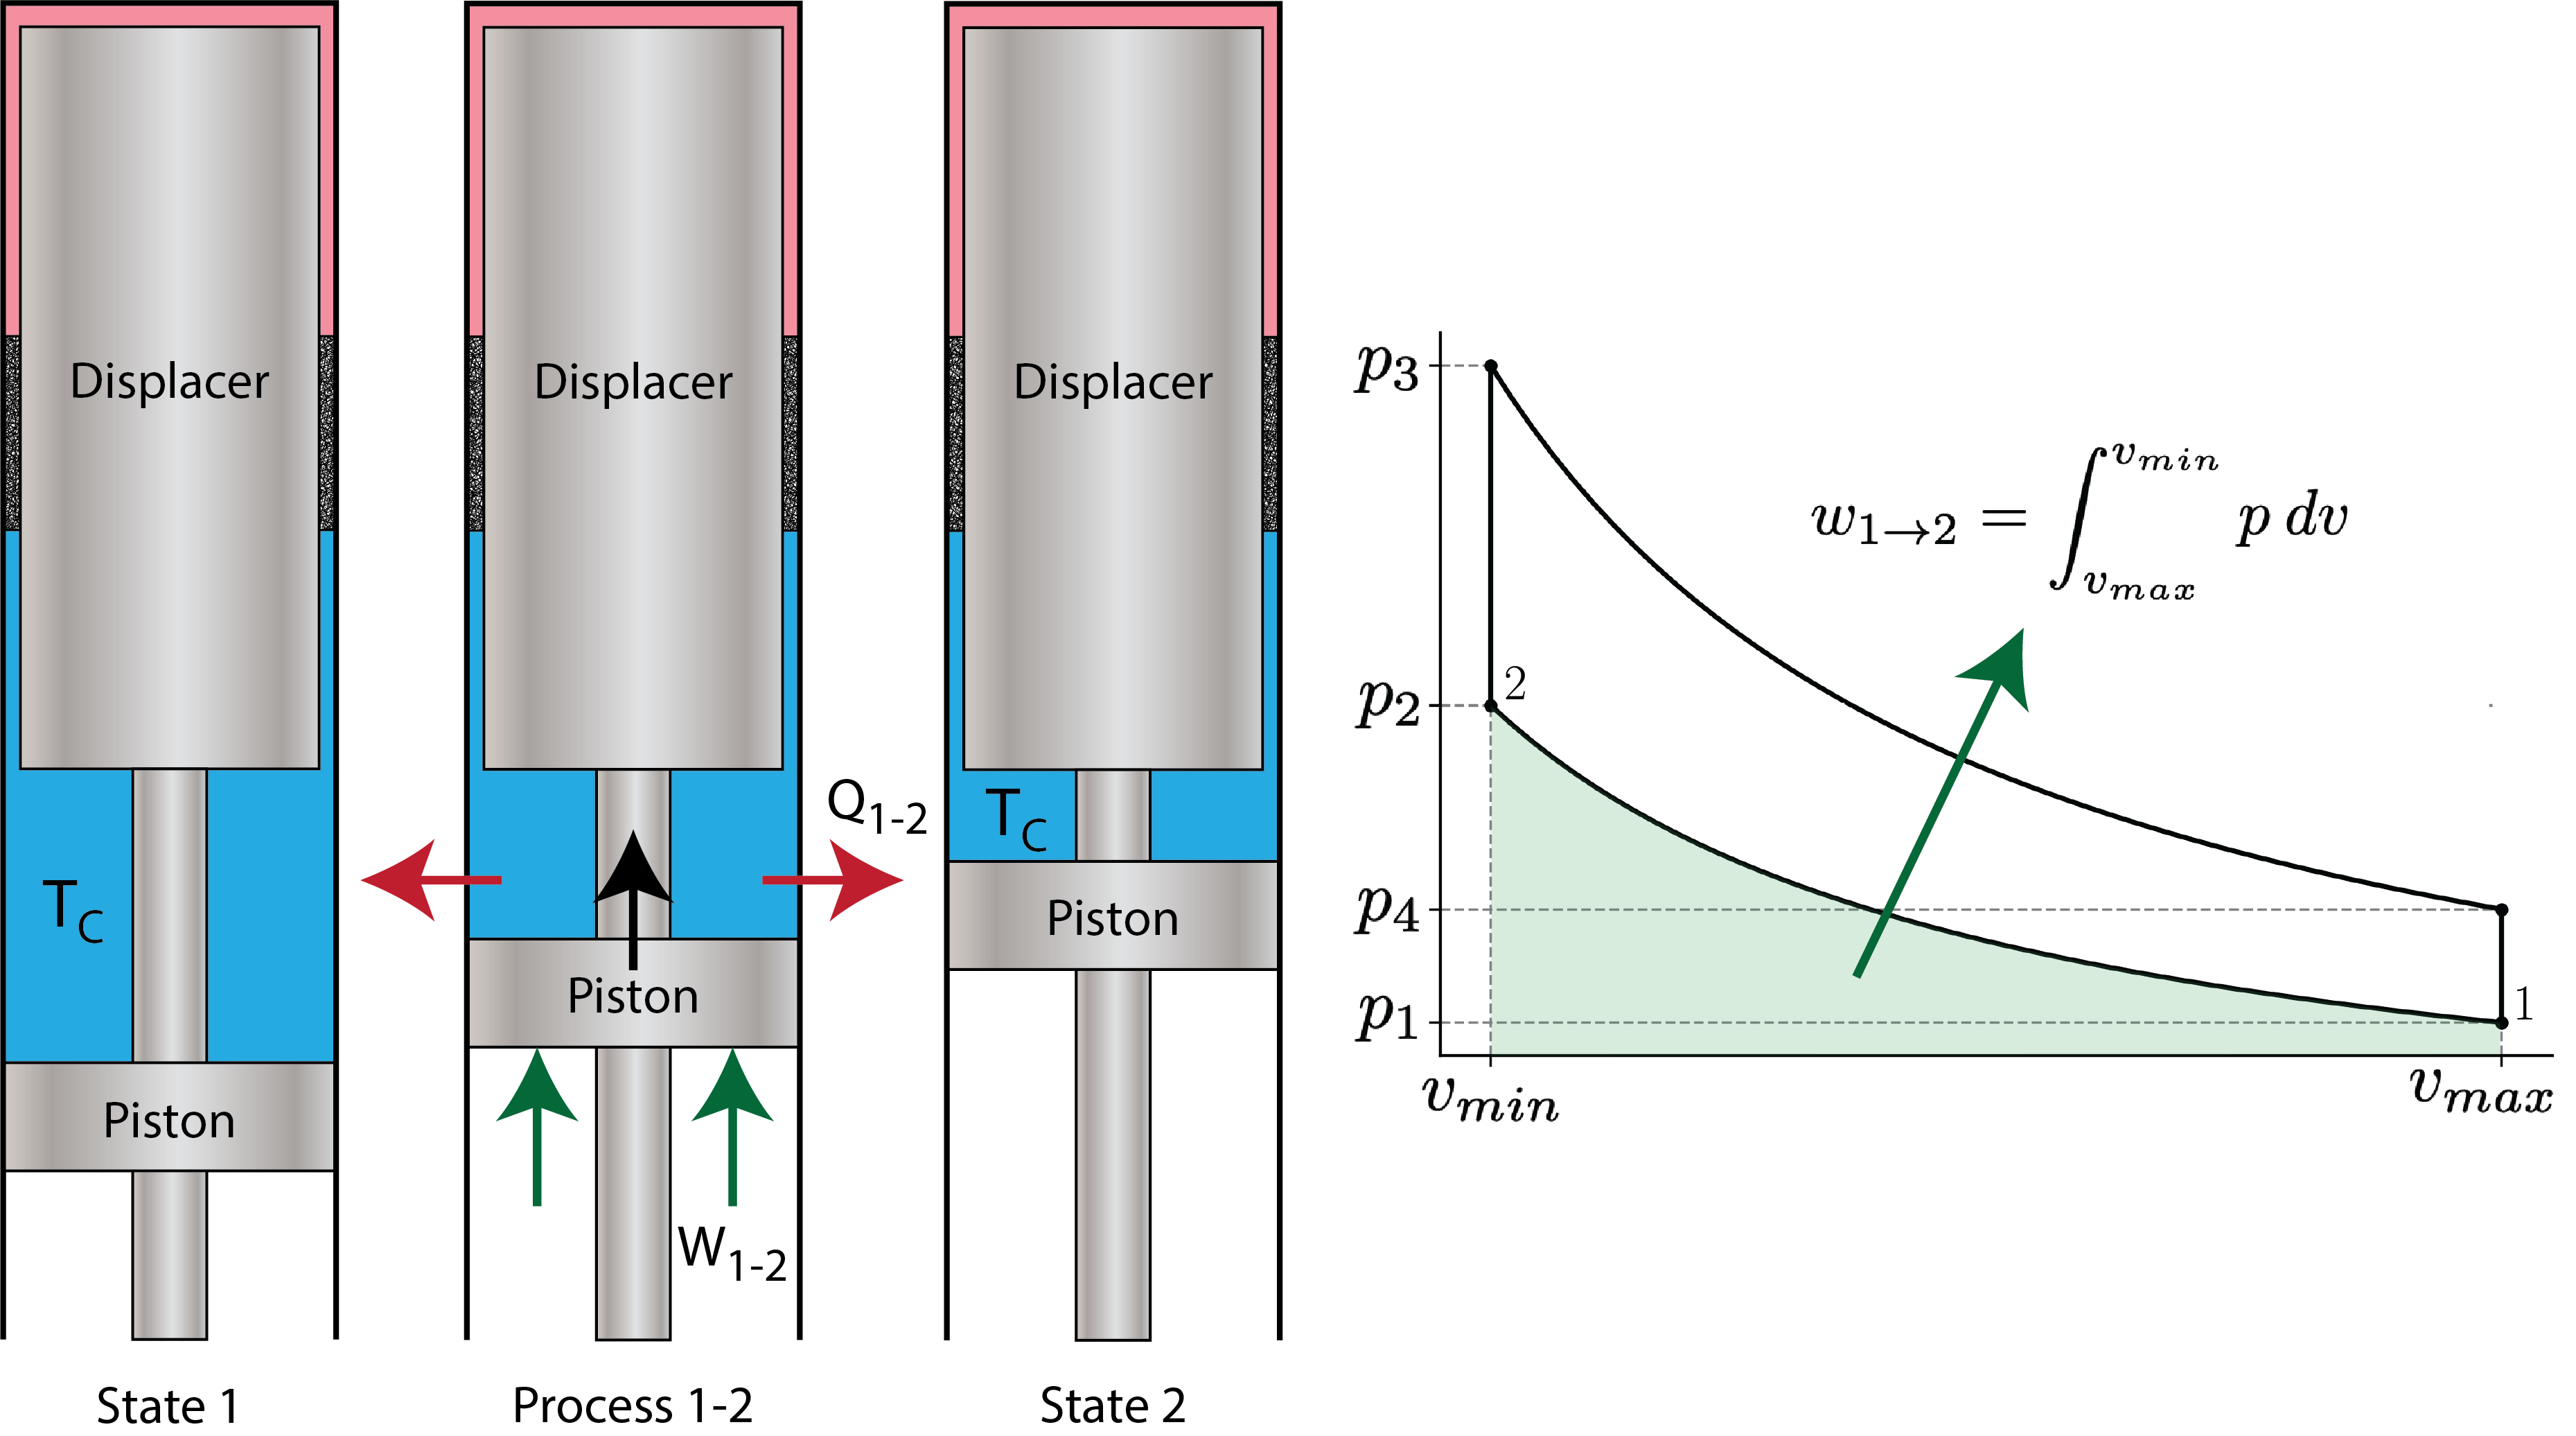
\includegraphics[width=0.9\textwidth]{StirlingEngineProcess1-2}
\caption{The compression process of the Stirling Engine.}
\label{fig:ch3_stirling12}
\end{figure}

Figure \ref{fig:ch3_stirling12} shows the compression from State 1 to State 2.  In process 1-2, the gas is compressed by the piston while the displacer is at the top of the cylinder. Thus during this process the gas is cooled in order to maintain a constant temperature $T_C$.  Note that without cooling, the work added by compression would increase the internal energy, and by extension temperature.

The work $W_{1-2}$ required to compress the gas is shown as the area under the $p$-$V$ curve, and is evaluated as follows, using the ideal gas law with the constant temperature during compression to say $p = \frac{R T_C}{v}$.

\begin{equation} \label{eq:stirlingCompWork}
  w_{1-2} = \int_{v_1}^{v_2} p\:dv=R T_C \int_{v_1}^{v_2} \frac{dv}{v}=RT_C\cdot  \ln\left(\frac{v_2}{v_1}\right)
\end{equation}

Another consequence of the constant temperature is that the internal energy of the gas will also stay unchanged.

\begin{equation}
  q_{1-2} - w_{1-2} = \cancelto{0}{\Delta u_{1-2}} \quad \rightarrow \quad q_{1-2} = w_{1-2}
\end{equation}

% --------------------------------------------------------------------
\subsection{Process 2$\rightarrow$3 -- Constant Volume Heating}

After compression, the displacer piston pushes the air from the cold region to the hot region, warming it up as it moves through the regeneration matrix.

\begin{figure}[H]
\centering
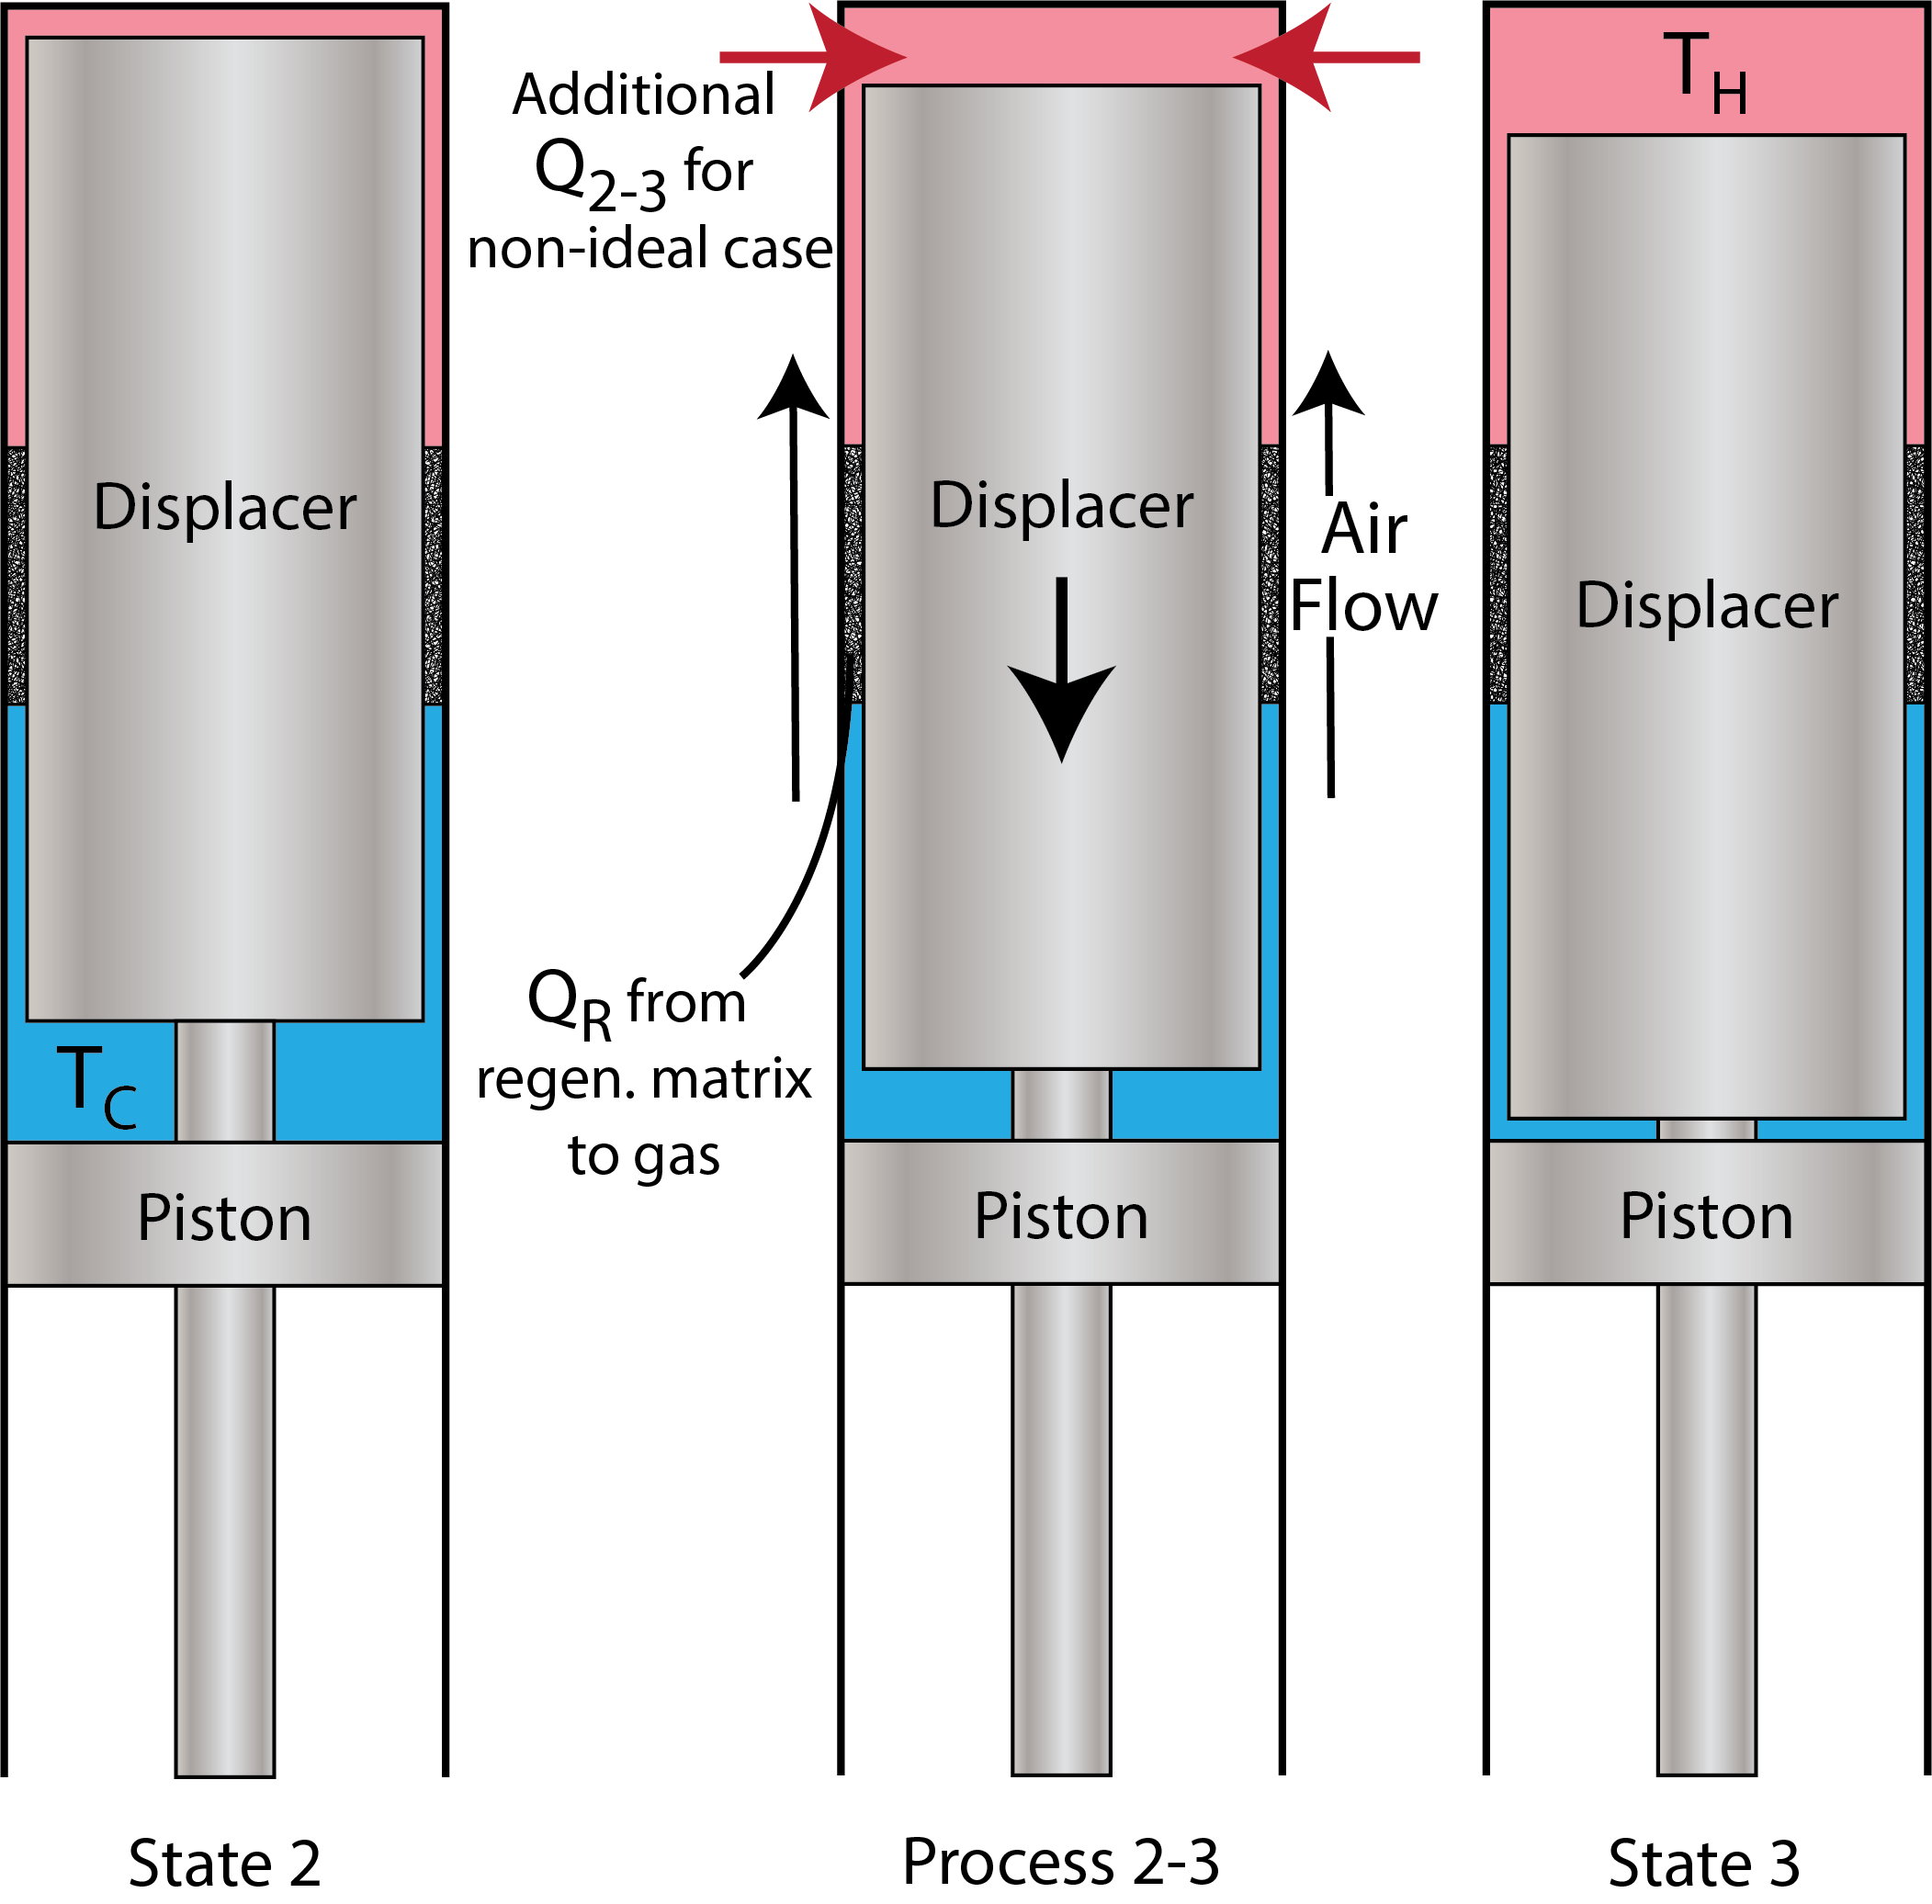
\includegraphics[width=0.6\textwidth]{StirlingEngineProcess2-3}
\caption{The heating process of the Stirling Engine.}
\label{fig:ch3_stirling23}
\end{figure}


Figure \ref{fig:ch3_stirling23} shows the movement of the displacer down into the cold region.  This in turn drives the air through the regenerator into the hot region.  The end result of this is that the air is significantly heated and ends up at $T_H$.

Importantly, there is no compression or expansion in Process 2-3.  This means no work is done between the two states, greatly simplifying our analysis:
\begin{equation} \label{eq:stirlingRegenerator}
  \Delta u_{2-3} = q_{2-3} - \cancelto{0}{w_{2-3}} \quad \rightarrow \quad q_{2-3} = c_v \left(T_H - T_C\right)
\end{equation}

% --------------------------------------------------------------------
\subsection{Process 3$\rightarrow$4 -- Isothermal Expansion}

After the air is displaced, the hot air expands, forcing back the piston.  Once again, this process is isothermal, but this time at a temperature $T_H$.

Figure \ref{fig:ch3_stirling34} shows Process 3-4, the expansion of the air at constant temperature.  The analysis mirrors that of Process 1-2.

\begin{figure}[H]
\centering
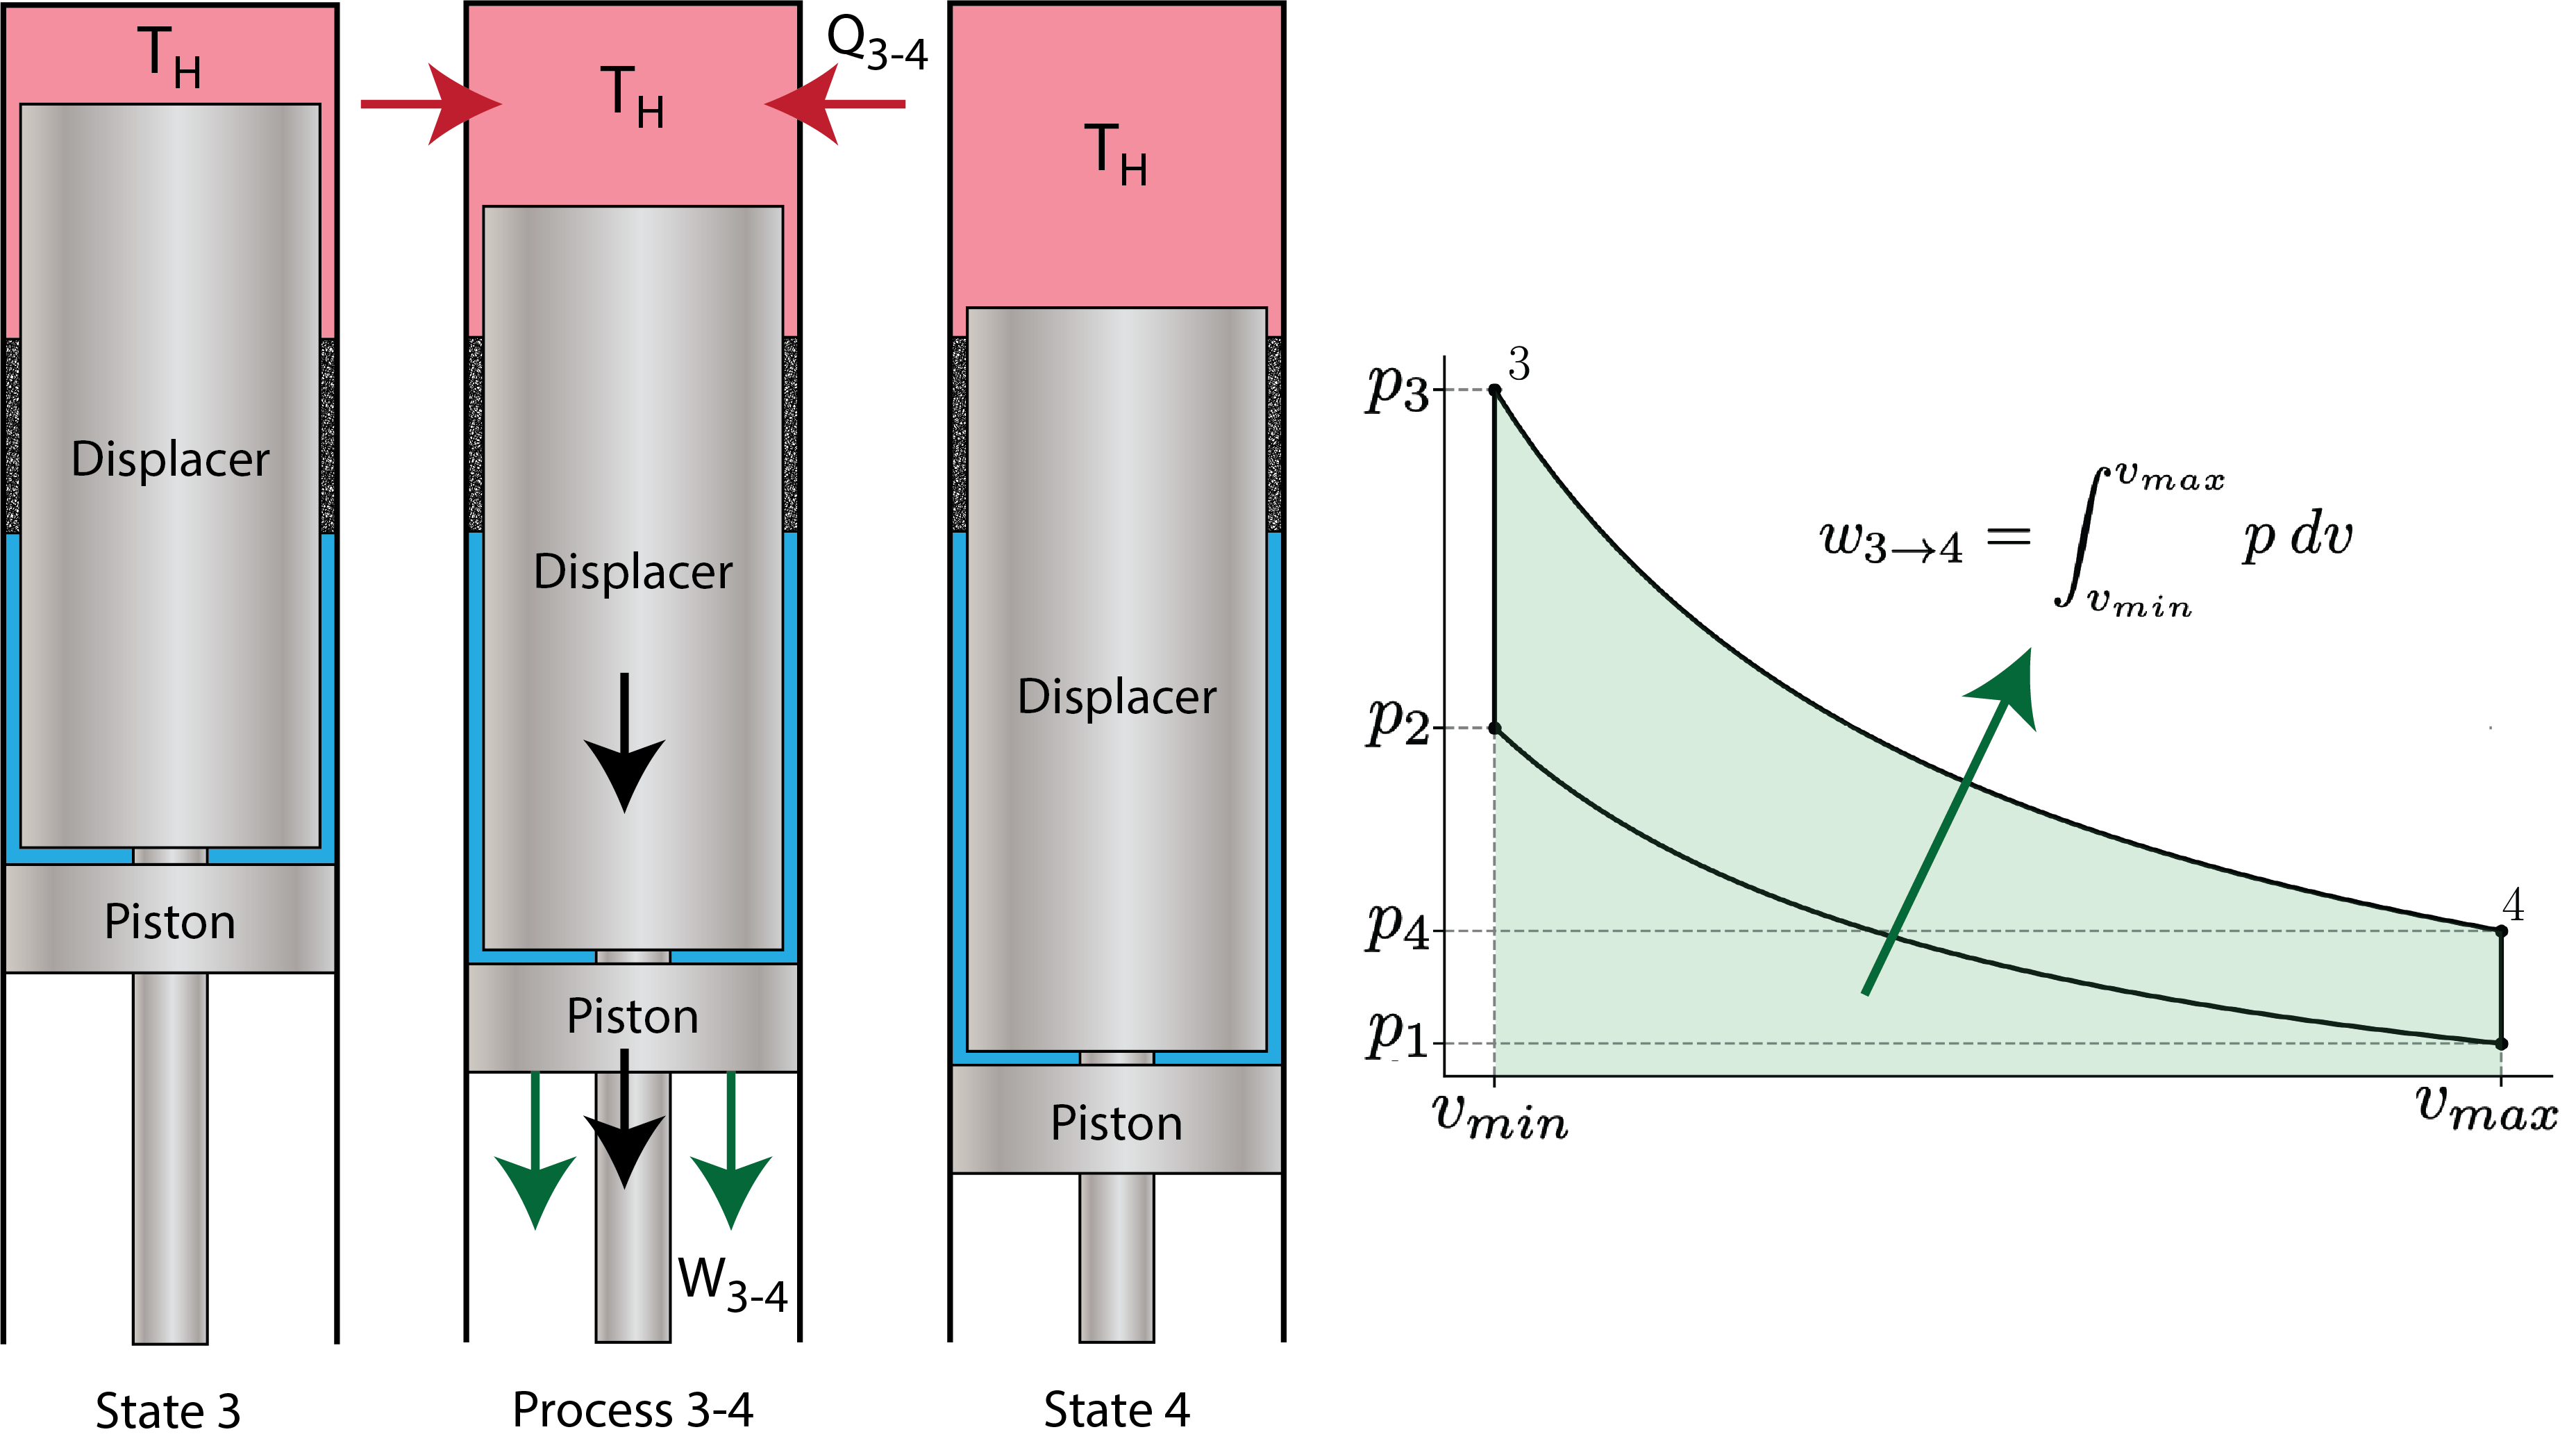
\includegraphics[width=0.9\textwidth]{StirlingEngineProcess3-4}
\caption{The expansion process of the Stirling Engine.}
\label{fig:ch3_stirling34}
\end{figure}

\begin{equation} \label{eq:stirlingExpWork}
  w_{3-4} = \int_{v_3}^{v_4} p\:dv= R T_H \int_{v_3}^{v_4} \frac{dv}{v}=RT_H\cdot  \ln\left(\frac{v_4}{v_3}\right)
\end{equation}

Fortunately, because Processes 2-3 and 4-1 are isometric (constant volume), we can make the replacements $v_3 \rightarrow v_2$ and $v_4\rightarrow v_1$ in Equation \ref{eq:stirlingExpWork}:

\begin{equation}
  w_{3-4} = RT_H \cdot \ln\left(\frac{v_1}{v_2}\right) = - \frac{T_H}{T_C} w_{1-2}
\end{equation}
\newpage
% --------------------------------------------------------------------
\subsection{Process 4$\rightarrow$1 -- Constant Volume Cooling}

Finally, Process 4-1 (shown in Figure \ref{fig:ch3_stirling41}) is essentially Process 2-3 in reverse (though with a larger volume).  The gas loses its heat to the regenerator matrix and is cooled back to $T_C$.

\begin{figure}[H]
\centering
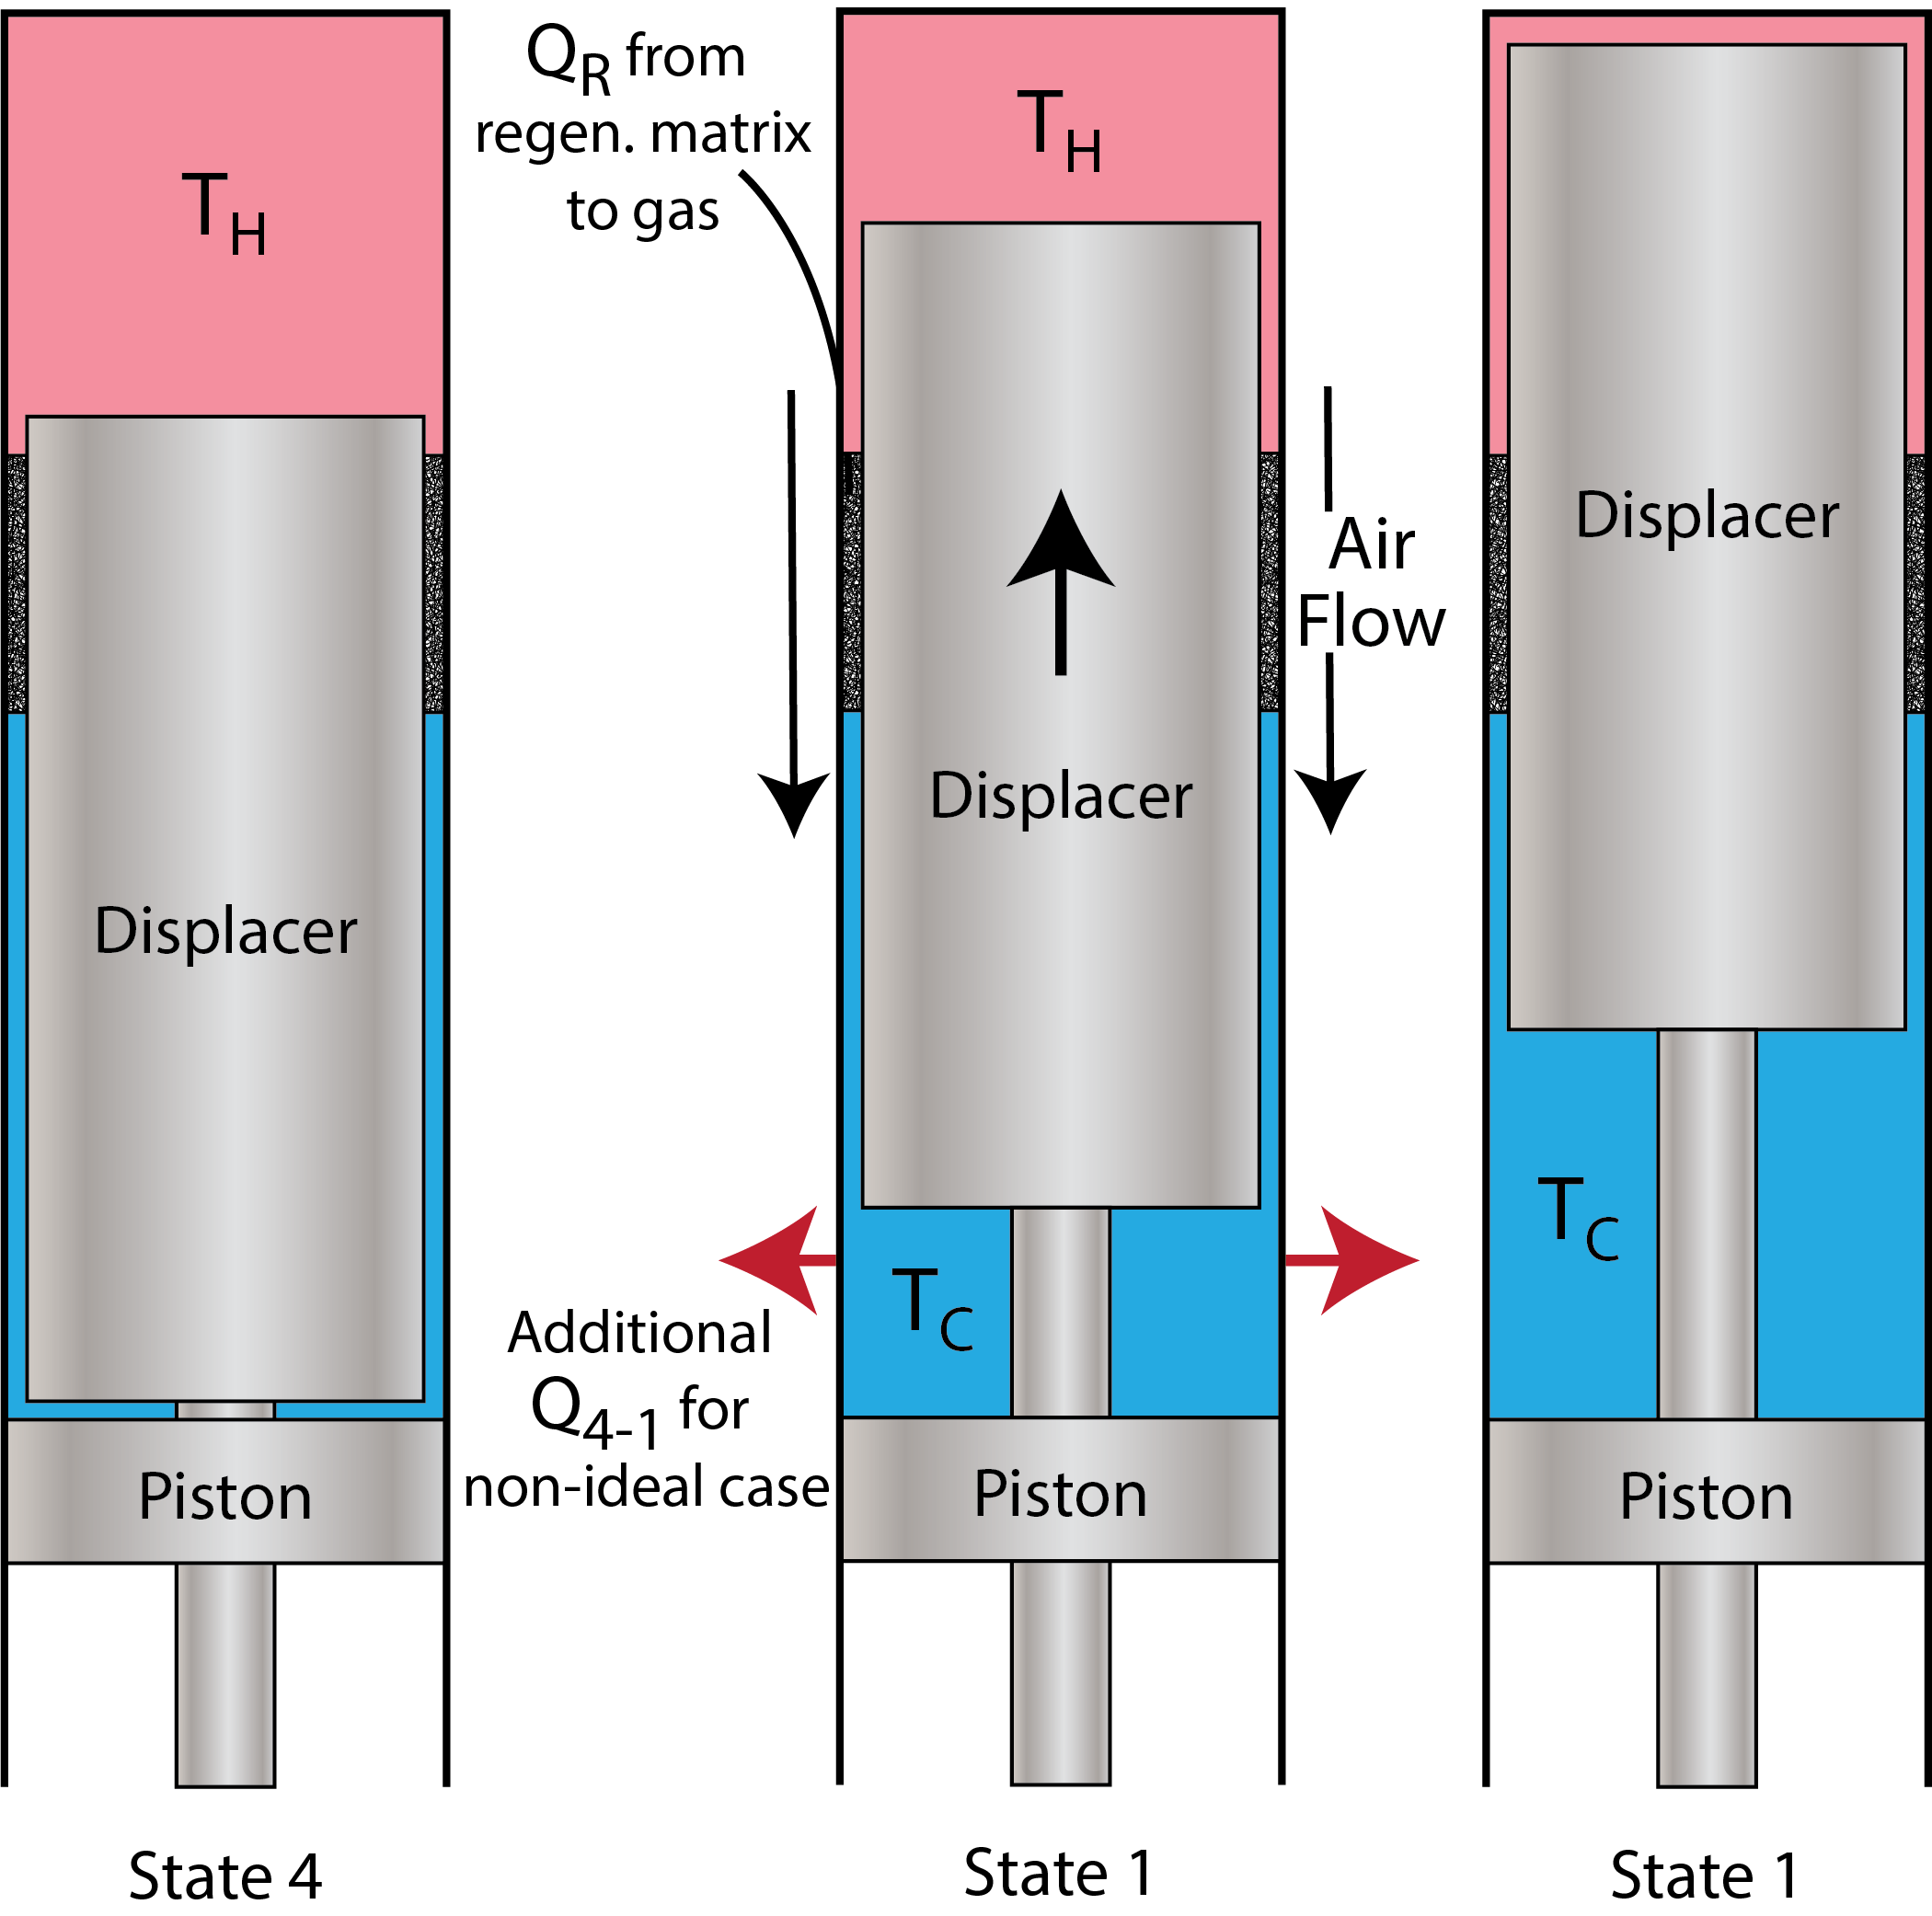
\includegraphics[width=0.6\textwidth]{StirlingEngineProcess4-1}
\caption{The cooling process of the Stirling Engine.}
\label{fig:ch3_stirling41}
\end{figure}

Again, the heat transfer is purely based on the change in temperature, as there is no work involved: $q_{4-1} = -c_v (T_H-T_C)$.  The sign is opposite of that for $q_{2-3}$ since we are cooling, rather than heating.

% --------------------------------------------------------------------
\subsection{Ideal Stirling Cycle Analysis}
For cycles, it is often helpful to write out the energy equation in tabular format, as shown in Table \ref{tab:ch3_stirling}.

\begin{table}[H]
  \centering
\def\arraystretch{1.5}
\caption{Tabular Representation of Energy Equation for Stirling Cycle}
\label{tab:ch3_stirling}
\begin{tabular}{r|ccc}
            & $\Delta u$        & $q$                                     & $w$                                    \\ \hline
Process 1-2 & 0                 & $-RT_C\cdot \ln\left(\frac{v_1}{v_2}\right)$ & $-RT_C\cdot \ln\left(\frac{v_1}{v_2}\right)$ \\
Process 2-3 & $ c_v (T_H-T_C)$ & $ c_v (T_H-T_C)$                        & 0                                      \\
Process 3-4 & 0                 &  $RT_H\cdot \ln\left(\frac{v_1}{v_2}\right)$ & $RT_H\cdot \ln\left(\frac{v_1}{v_2}\right)$ \\ 
Process 4-1 & $- c_v (T_H-T_C)$& $- c_v (T_H-T_C)$                        &  0                                    \\ \hhline{=|===}
Total (net) & 0                 & $R(T_H-T_C)\cdot \ln\left(\frac{v_1}{v_2}\right)$ & $R(T_H-T_C)\cdot \ln\left(\frac{v_1}{v_2}\right)$
\end{tabular}
\def\arraystretch{1.0}
\end{table}

We expect that $\Delta u$ for a cycle is always zero, as the cycle starts and ends at the same point.  This implies in turn that $q_{net} = w_{net}$, which is exactly what we see in Table \ref{tab:ch3_stirling}.  In fact, the purpose of the Stirling engine is to turn the net heat transfer into work.  The heat transfer to and from the regenerator doesn't come into play, as the heat transfer in Process 2-3 perfectly cancels with the heat transfer in Process 4-1.  The total work done (and the total heat added to the system) can be simplified to:

\begin{equation} \label{eq:ch3_netWorkStirling}
  q_{net} = w_{net} = R\Delta T\cdot \ln (r)
\end{equation}

where $\Delta T$ is the difference between the hot and cold temperatures and $r$ is the {\bf compression ratio}, defined as:
\begin{equation}\label{eq:ch3_compressionRatio}
  r = \frac{v_{\rm max}}{v_{\rm min}}=\frac{V_{\rm max}}{V_{\rm min}}
\end{equation}
We can also define the {\bf thermal efficiency} as the ratio between the input heat and the net work.  This efficiency is a picture of how much work we can get out of an engine based on the amount of fuel we burn.
\begin{align} \label{eq:ch3_StirlingEfficiency}
  \nonumber \eta_{th} &= \frac{w_{net}}{q_{in}} = \frac{w_{net}}{q_{3-4}} = \frac{R\Delta T\cdot \ln (r)}{RT_H\cdot \ln(r)} \\
  \eta_{th} &= \frac{\Delta T}{T_H} = 1 - \frac{T_C}{T_H}
\end{align}

Equation \ref{eq:ch3_StirlingEfficiency} is the maximum theoretical efficiency achievable from a heat engine, and is typically referred to as the {\bf Carnot efficiency}.

% --------------------------------------------------------------------
\subsection{Stirling Engines without Regeneration}
Note that the ideal case assumes that the regenerator is able to fully heat/cool the air in Processes 2-3 and 4-1.  If this is not the case (or if there is no regenerator present), then the extra heat $Q_{2-3}$ must be provided by the heater, which will reduce the efficiency.  In the case of no regenerator, the efficiency becomes:
\begin{equation} \label{eq:ch3_StirlingEfficiencyNoRegen}
  \nonumber \eta_{th} = \frac{w_{net}}{q_{in} + q_{2-3}} = \frac{R\Delta T\cdot \ln (r)}{(RT_H\cdot \ln(r)+c_v\Delta T)}
\end{equation}

This is a little difficult to draw conclusions from, but let's look at a sample case with air as the working fluid ($c_v \approx 2.5 R$), $T_C = 300\ {\rm K}$, $T_H = 600\ {\rm K}$, and $r = 1.3$.  That gives us an ideal thermal efficiency of $\eta_{th, {\rm regen}} = 0.5$ with the regenerator, and an ideal thermal efficiency of $\eta_{th, {\rm no\ regen}} = 0.097$!  Having a regenerator is hugely important!

Another important note is that even with a regenerator, the practical Stirling cycle has many losses associated with it and does not really involve isothermal processes, nor ideal regeneration. Furthermore, Stirling cycle machines do not typically start and stop the pistons perfectly, meaning that the $p$-$V$ diagram has a more oval shape, rather than the sharp edges defined in the above diagrams. Nevertheless we use the ideal Stirling cycle to get an initial understanding and appreciation of the cycle performance.
\newpage
\begin{example}{Stirling Cycle Engine/Generator} 
  This exercise concerns the ideal performance of the \href{https://www.microgen-engine.com/engines/}{Microgen 1050 Watt engine} which is gas fired and was designed to generate electricity (1kWe) as well as to provide hot water for a private home. This engine has a similar configuration to the Stirling engine discussed in Section \ref{sec:idealStirling}.  (Note that the values presented here are not actual values of the Microgen Engine, however were devised by your instructor for purposes of this exercise only).

  The working fluid is helium, which has an gas constant $R$ = 2.077 kJ/kg K, and constant volume specific heat $c_v$ = 3.116 kJ/kg K. (refer: Ideal Gas Properties).  State (1) is defined at a maximum volume of 650 $\rm cm^3$ and a pressure of 10 bar, and State (2) is defined at a minimum volume of 550 $\rm cm^3$.  Process 1-2 is isothermal compression at $T_C$ = 50°C, Process 2-3 is isometric heating, using a regenerator to source the heat.  Process 3-4 is isothermal expansion at $T_H$ = 500°C, and Process 4-1 is isometric cooling, again using the regenerator as a heat sink.
  \begin{enumerate}[a)]
  \item From the given conditions at state 1 determine the mass of working gas (helium) used in the cycle.
    
  \item Determine the net work done per cycle (kiloJoules): $W_{exp}$ + $W_{comp}$ (Note that the compression work $W_{comp}$ is always negative). At a frequency of 50 Hertz (cycles per second) determine the power output produced by the engine.
    
  \item Determine the heat absorbed in the expansion space $Q_{in}$ during the expansion process (3)-(4).
    
  \item Evaluate the Thermal Efficiency $\eta_{th}$, defined as: $\eta_{th} = (W_{exp} + W_{comp}) / Q_{in}$. (Net mechanical work done divided by the heat supplied externally by the gas burner).
    
  \item Determine the amount of thermal power rejected to the cooling water. Note that at a temperature of 50°C this is suitable for providing hot water for the home, as well as providing home space heating capability.
    
  \item Determine the amount of heat transferred to the working fluid $Q_R$ as it passes through the regenerator during process (2)-(3). If this heat were to be supplied externally by the gas burner, (i.e. no regenerator) what would be the new value of thermal efficiency $\eta_{th}$? 
  \end{enumerate}
  
  {\bf Solution Approach}
  \begin{enumerate}[a)]
  \item  We can find the mass through the ideal gas law, letting 1 $\rm cm^3$ = $1\times 10^{-6}m^3$:
    \begin{align*}
      p_1v_1=RT_1 \quad\quad \rightarrow & \quad\quad v_1 = \frac{RT_1}{p_1} \\
      & \quad\quad v_1 = \frac{2.077 {\rm\ kJ/kgK} \cdot 323.15{\rm\ K}}{1000\ \rm kPa} \\
      & \quad\quad \redbox{v_1 = 0.6712 \rm\ m^3/kg} \\
      v_1 = \frac{V_1}{m} \quad\quad \rightarrow & \quad\quad \redbox{m = \frac{6.5\times 10^{-4} \rm\ m^3}{0.6712\ \rm m^3/kg} = 9.68\times 10^{-4}\ \rm kg}
    \end{align*}
  \item The net work comes from Equation \ref{eq:ch3_netWorkStirling}:
    \begin{align*}
      W_{net} &= m R \left(T_H-T_C\right) \ln{\left(\frac{V_1}{V_2}\right)} \\
      W_{net} &= ({0.968\ \rm g}) \left(2.077\frac{\rm kJ}{\rm kg K}\right) (450\ {\rm K}) \ln{\left(\frac{650\ \rm cm^3}{550\ \rm cm^3}\right)} \quad\rightarrow\quad \redbox{W_{net} = 0.151\ \rm kJ}
    \end{align*}
    We can convert from work to power by multiplying by the frequency (units of Hz are the same as 1/s):
    \begin{equation*}
      \dot{W}_{net} = W_{net} \cdot f = {0.151\ \rm kJ} \cdot 50 \frac{1}{\rm s} \quad\rightarrow\quad \redbox{\dot{W}_{net} = 7.55\rm\ kW}
    \end{equation*}
  \item The heat absorbed in the expansion space can be calculated from Equation \ref{eq:stirlingExpWork}, recognizing that the constant-temperature process results in no change in internal energy:
    \begin{align*}
      W_{exp} &= Q_{exp} = m R T_H \ln{\left(\frac{V_4}{V_3}\right)} \\
      Q_{exp} &= ({0.968\ \rm g}) \left(2.077\frac{\rm kJ}{\rm kg K}\right) (773.15\ {\rm K}) \ln{\left(\frac{650\ \rm cm^3}{550\ \rm cm^3}\right)} \ \rightarrow\ \redbox{Q_{exp} = 0.260\ \rm kJ}
    \end{align*}
    This is equivalent to $\redbox{\dot{Q}_{exp} = 13.0\rm\ kJ}$.
  \item We can find the thermal efficiency from the results of the previous two parts:
    \begin{equation*}
      \eta_{th} = \frac{W_{net}}{Q_{in}} = \frac{0.151\rm\ kJ}{0.260\rm\ kJ} \quad\rightarrow\quad \redbox{\eta_{\th} = 58\%}
    \end{equation*}
  \item The heat rejected to the cooling water can be calculated directly as in part c), or by recognizing that $Q_{in} - Q_{out} = W_{net}$.
    \begin{equation*}
      Q_{out} = Q_{in} - W_{net} = 0.260{\rm\ kJ} - 0.151{\rm\ kJ} \quad\rightarrow\quad \redbox{Q_{out} = 0.109{\rm\ kJ}}
    \end{equation*}
  \item The regenerator transfers enough heat to change the temperature of the helium from 50°C to 500°C.  This heat can be calculated through the definition of the $c_v$, as in Equation \ref{eq:stirlingRegenerator}:
    \begin{equation*}
      Q_R = m c_v \Delta T = ({0.968\ \rm g})\left(3.116\frac{\rm kJ}{\rm kg K}\right) (450\ {\rm K}) \quad\rightarrow\quad \redbox{Q_R = 1.36\rm\ kJ}
    \end{equation*}
    Adding the regenerator heat transfer to the heat supplied to the gas burner allows us to find the new thermal efficiency:
    \begin{equation*}
      \eta_{th} = \frac{W_{net}}{Q_{in}+Q_R} = \frac{0.151\rm\ kJ}{0.260\rm\ kJ + 1.35\rm\ kJ} \quad\rightarrow\quad \redbox{\eta_{th} = 9.3\%}
    \end{equation*}
    This value is in line with the efficiency calculated in the previous section.
  \end{enumerate}
  
\end{example}

% --------------------------------------------------------------------
\section{Stirling Cycle Cooling} \label{sec:ch3_StirlingCooling}
% --------------------------------------------------------------------

One important aspect of Stirling cycle machines that we need to consider is that the cycle can be reversed - if we put net work into the cycle then it can be used to pump heat from a low temperature source to a high temperature sink.  This results in a very compact refrigerator, which can reach very low temperatures.  This technology has been used in a few specific instances, primarily in \href{https://www.stirlingultracold.com}{ultra-low-temperature freezers for biomedical uses}.  The cycle used in standard air conditioning units is discussed in Section \ref{sec:Refrigeration}.

\begin{figure}[H]
\centering
\scalebox{1}[-1]{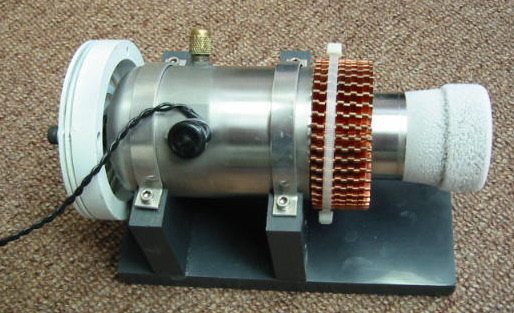
\includegraphics[angle=180, width=0.75\textwidth]{StirlingCooler}}
\caption{The M100B Stirling Cooler from Global Cooling (now Stirling Ultracold).}
\label{fig:ch3_stirlingCooler}
\end{figure}

Figure \ref{fig:ch3_stirlingCooler} shows an example of a Stirling Cooler.  Power is provided through the small electrical cord, while ice crystals can be seen forming on the left-hand side of the cooler.  Refer to the schematic in Figure \ref{fig:ch3_M100BSchematic} to identify the various parts of the cooler.

\begin{figure}[H]
\centering
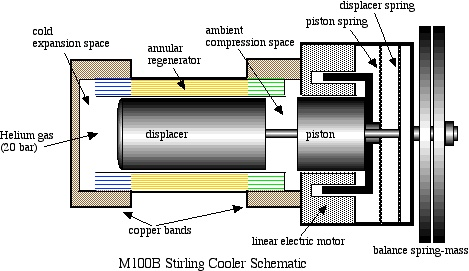
\includegraphics[width=0.75\textwidth]{M100Bschem}
\caption{Schematic of M100B Stirling Cooler from Global Cooling.}
\label{fig:ch3_M100BSchematic}
\end{figure}

%Conceptually the cooler is an extremely simple device, consisting essentially of only two moving parts - a piston and a displacer. The displacer shuttles the working gas (helium) between the compression and expansion spaces. The phasing between the piston and displacer is such that when the most of the gas is in the ambient compression space then the piston compresses the gas while rejecting heat to the ambient. The displacer then displaces the gas through the regenerator to the cold expansion space, and then both displacer and piston allow the gas to expand in this space while absorbing heat at a low temperature.

Figure \ref{fig:ch3_StirlingCoolingCycle} shows the cycle used by the Stirling Cooler.  Heat is rejected to the environment ($Q_H$) in Process 1-2, rejected to the regenerator ($Q_R$) in Process 2-3, absorbed from the refrigerated space ($Q_C$) in Process 3-4, and finally absorbed from the regenerator ($Q_R$) in Process 4-1. More work is required to drive Process 1-2 than is regained in Process 3-4, meaning that the net work for this cycle is negative.  In other words, work is required to move heat from the cold side to the hot side.

\begin{figure}[H]
\centering
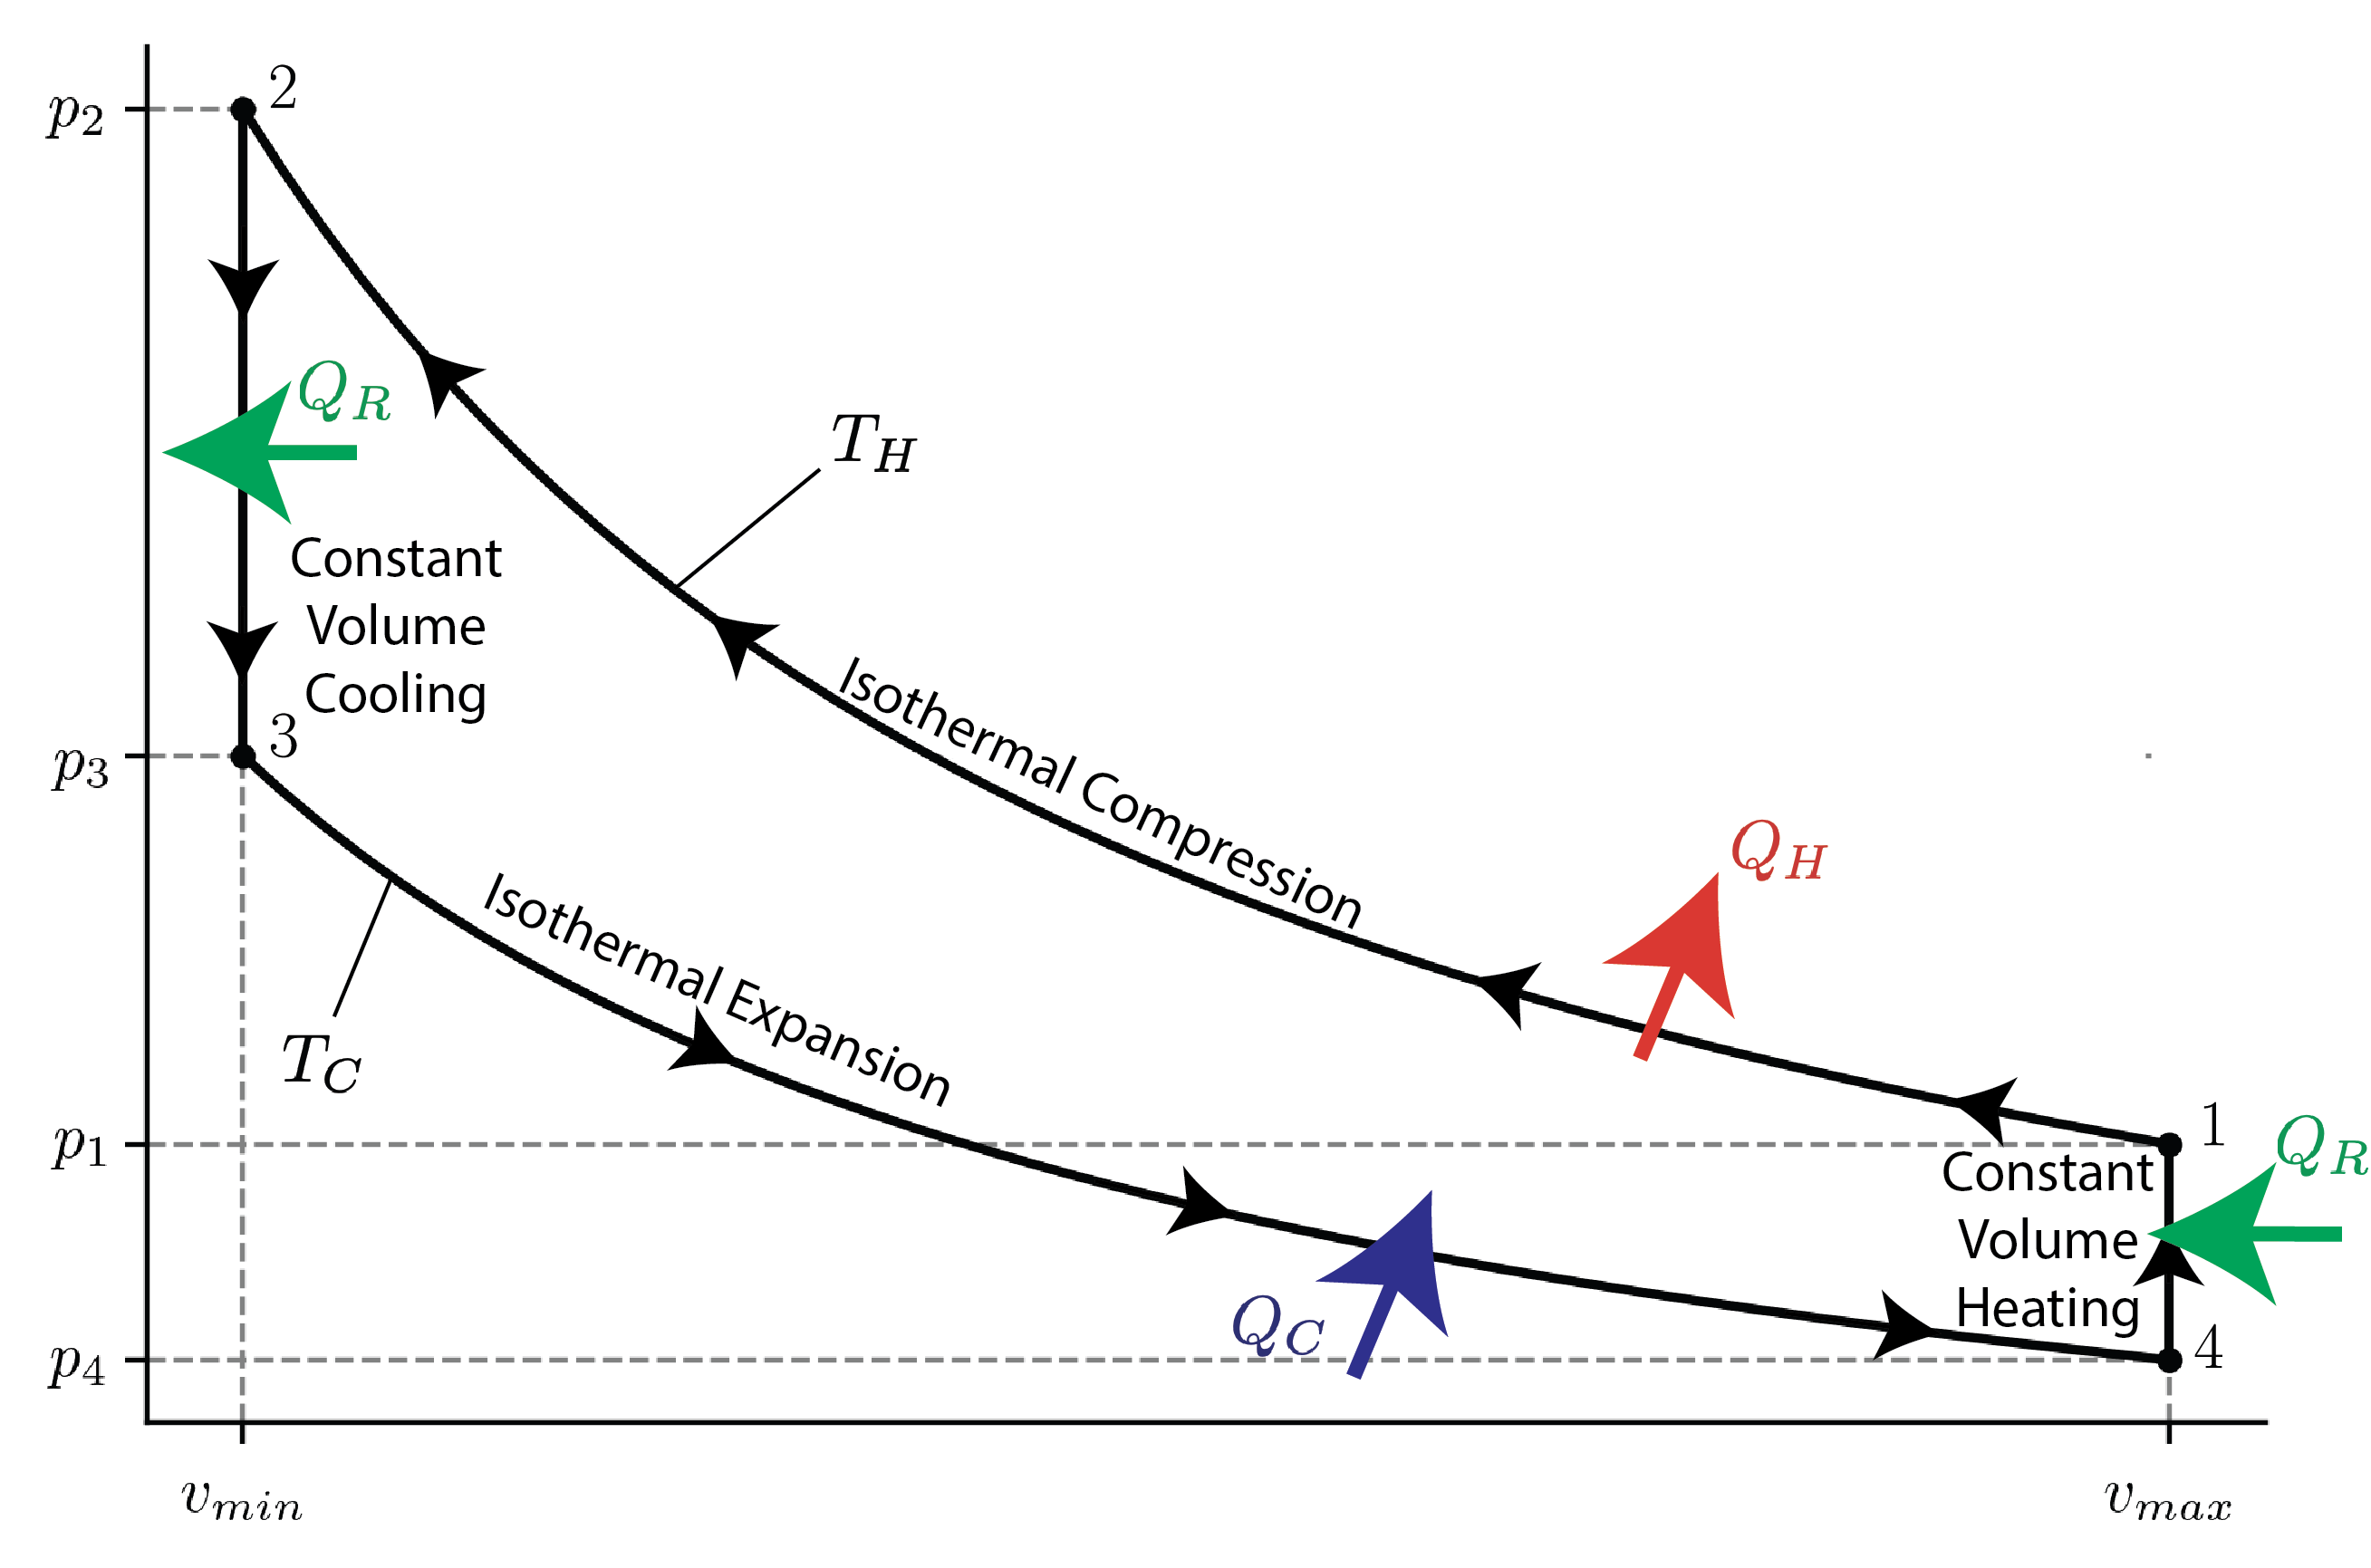
\includegraphics[width=0.75\textwidth]{StirlingCoolingDiagram}
\caption{$p$-$v$ diagram of the Stirling Cooling Cycle.}
\label{fig:ch3_StirlingCoolingCycle}
\end{figure}

Cooling cycles do not use the thermal efficiency as an indicator of performance.  Following the general idea that ``efficiency'' is ``what we get out''/''what we put in'', the efficiency of a cooling cycle is defined at the Coefficient of Performance for a refrigeration cycle, $COP_R$:
\begin{equation*}
  COP_R = \frac{q_{in}}{w_{net}}
\end{equation*}

The heat absorbed, $q_{in}$, is the benefit we get from the cooling cycle, as we are seeking to remove heat from a refrigerated space.  The net work, $w_{net}$, is what we have to pay to get that benefit, as we are doing work on the cycle.

Conversely, if we chose to think of this cycle as a way to add heat to a heated space, we would arrive at the Coefficient of Performance for a heat pump cycle, $COP_{HP}$:
\begin{equation*}
  COP_{HP} = \frac{q_{out}}{w_{net}}
\end{equation*}

In this case, the heat rejected to the heated space is the benefit from the cycle, which leads to a change in our ``efficiency'' calculations.

Example \ref{ex:StirlingCooling} investigates the Stirling cooling cycle in more detail.
\newpage
\begin{example}[label={ex:StirlingCooling}]{Stirling Cycle Cooling}

  A Stirling cooling cycle is defined as follows:
  \begin{itemize}
  \item Compression occurs at a constant temperature of $T_H$ = 30°C.
  \item Expansion occurs at a constant temperature of $T_C$ = -20°C.
  \item The maximum volume is 35 $\rm cm^3$
  \item The minimum volume is 30 $\rm cm^3$
  \item The pressure immediately before compression is 1.9 MPa.
  \item The working fluid is helium, which has an gas constant $R$ = 2.077 kJ/kg K, and constant volume specific heat $C_v$ = 3.116 kJ/kg K.
  \end{itemize}

\begin{enumerate}[a)]
\item Determine the heat absorbed in the expansion stroke (Joules). Determine also the heat power absorbed (Watts). Note that the cycle frequency is the line frequency (f = 60 Hz).

\item Determine the net work done per cycle (Joules): $W_{net} = W_{comp} + W_{exp}$ (Note that the compression work $W_{comp}$ is always negative). Determine also the power supplied to the linear electric motor (Watts).
  
\item Evaluate the Coefficient of Performance of the refrigerator defined as: $COP_R = Q_C / W_{net}$. (heat absorbed in the expansion space divided by the net work done). 

\item Determine the amount of heat rejected by the working fluid $Q_R$ as it passes through the regenerator matrix during constant volume cooling.

\item If there were no regenerator present then this heat would need to be removed from the gas by the expansion process in order to reduce the temperature to the cold temperature of the freezer. How would this affect the performance of the cooler? Discuss the importance of an effective regenerator in the Stirling cycle cooler.
\end{enumerate}

{\bf Solution Approach}

First off, let's find the mass of the working fluid.

For the first state, pressure and temperature are both defined, as is the total volume.  This is sufficient for us to find the mass of the working fluid.  As part of the process, we need to convert 35 $\rm cm^3$ to $3.5\times 10^{-5} \rm m^3$.
\begin{align*}
  p_1v_1=RT_1 \quad\quad \rightarrow & \quad\quad v_1 = \frac{RT_1}{p_1} \\
  & \quad\quad v_1 = \frac{2.077 {\rm\ kJ/kgK} \cdot 303.15{\rm\ K}}{1900\ \rm kPa} \\
  & \quad\quad \redbox{v_1 = 0.3314 \rm\ m^3/kg} \\
  v_1 = \frac{V_1}{m} \quad\quad \rightarrow & \quad\quad \redbox{m = \frac{3.5\times 10^{-5} \rm\ m^3}{0.3314\ \rm m^3/kg} = 1.056\times 10^{-4}\ \rm kg}
\end{align*}

\begin{enumerate}[a)]
\item Once we have the mass, we can use Table \ref{tab:ch3_stirling} for the analysis, except we need to replace $T_C$ with $T_H$ and vice-versa. The heat transfer is therefore:
  \begin{align*}
    Q_{exp} &= m R T_C \ln{\left(\frac{v_4}{v_3}\right)} = m R T_C \ln{\left(\frac{V_4}{V_3}\right)} \\
    Q_{exp} &= ({0.1056\ \rm g}) \left(2.077\frac{\rm kJ}{\rm kg K}\right) (253.15\ {\rm K}) \ln{\left(\frac{35\ \rm cm^3}{30\ \rm cm^3}\right)} \quad\rightarrow\quad \redbox{Q = 8.56\ \rm J}
  \end{align*}

  We can get to heat power absorbed simply by multiplying by the frequency of 60 Hz.
  \begin{equation*}
    \dot{Q}_{exp} = Q \cdot f = {8.56\ \rm J} \cdot 60 \frac{1}{\rm s} \quad\rightarrow\quad \redbox{\dot{Q}_{exp} = 513.6\rm\ W}
  \end{equation*}

\item The net work can be obtained from Equation \ref{eq:ch3_netWorkStirling}, again with $T_C$ and $T_H$ switched.
  \begin{align*}
    W_{net} &= m R \left(T_C-T_H\right) \ln{\left(\frac{V_1}{V_2}\right)} \\
    W_{net} &= ({0.1056\ \rm g}) \left(2.077\frac{\rm kJ}{\rm kg K}\right) (50\ {\rm K}) \ln{\left(\frac{35\ \rm cm^3}{30\ \rm cm^3}\right)} \quad\rightarrow\quad \redbox{W_{net} = -1.69\ \rm J}
  \end{align*}
  Note that the work done is negative, indicating that work is performed on the cycle, rather than provided by it.

  We can again find the power by multiplying by $f$.  This becomes $\redbox{\dot{W}_{net} = -101\rm\ W}$.
\item The Coefficient of Performance is easily determined from the two previous results.
  \begin{equation*}
    COP_R = \frac{Q_C}{W_{net}} = \frac{8.56\ \rm J}{1.69\ \rm J} \quad\rightarrow\quad \redbox{COP_R = 5.07}
  \end{equation*}

\item The heat absorbed/rejected by the regeneration matrix can be found from Equation \ref{eq:stirlingRegenerator}.
  \begin{equation*}
    Q_R = m c_v \Delta T = ({0.1056\ \rm g})\left(3.116\frac{\rm kJ}{\rm kg K}\right) (50\ {\rm K}) \quad\rightarrow\quad \redbox{Q_R = 16.45 J}
  \end{equation*}
  This equates to $\redbox{\dot{Q}_{R} = 988\rm\ W}$.
\item Without regeneration, we would expect a drastically lower $COP_R$ value.  It's difficult to see exactly how this comes about, as there is no easy mechanism through which we can compensate for the lack of a regenerator (like we simply added more heat in the Stirling engine).
\end{enumerate}


\end{example}

%% The process between state 1 and 2 is isothermal compression, meaning that $T_2 = T_1$, and $V_2$ is given as 35 $\rm cm^3$.  We can calculate the new pressure using the ideal gas law.  While we could plug in all the values directly, I prefer to create a ratio of the two ideal gas law equations, as follows:
%% \begin{align*}
%%   \frac{p_2}{p_1}\frac{v_2}{v_1} &= \cancel{\frac{R}{R}}\cancel{\frac{T_2}{T_1}} = 1 \\
%%   p_2 &= p_1 \frac{v_1}{v_2} \\
%%   p_2 &= 1.9 {\rm\ MPa} \cdot \frac{35 \rm\ cm^3}{30 \rm\ cm^3} \quad \rightarrow \quad \redbox{p_2 = 2.217\rm\ MPa}
%% \end{align*}
%% Process 2-3 is constant volume cooling to $T_3$ = -20°C.  We can again find the new pressure using the ratio of ideal gas law equations:
%% \begin{align*}
%%   \frac{p_3}{p_2}\cancel{\frac{v_3}{v_2}} &= \cancel{\frac{R}{R}}\frac{T_3}{T_2} = 1 \\
%%   p_3 &= p_2 \frac{T_3}{T_2} \\
%%   p_3 &= 2.217 {\rm\ MPa} \cdot \frac{253.15 \rm\ K}{303.15 \rm\ K} \quad \rightarrow \quad \redbox{p_3 = 1.851\rm\ MPa}
%% Process 3-4 is constant temperature expansion back to $V_4=V_1=35\rm\ cm^3$.  We can find $p_4$ the same way as before:
%% \begin{align*}
%%   \frac{p_4}{p_3}\frac{v_4}{v_3} &= \cancel{\frac{R}{R}}\cancel{\frac{T_4}{T_3}} = 1 \\
%%   p_4 &= p_3 \frac{v_3}{v_4} \\
%%   p_4 &= 1.851 {\rm\ MPa} \cdot \frac{30 \rm\ cm^3}{35 \rm\ cm^3} \quad \rightarrow \quad \redbox{p_4 = 1.586\rm\ MPa}
%% \end{align*}



% --------------------------------------------------------------------
\section{Ideal Gas Adiabatic Processes} \label{sec:ch3_idealGasAdiabatic}
The next two cycles both rely heavily on {\bf adiabatic} processes.  In order to discuss those cycles, we will look closer at adiabatic processes for an ideal gas.

Adiabatic processes are simply processes without heat transfer.  This means that the change in internal energy is purely due to the work done.

\begin{equation*}
  \cancelto{0}{\delta q} - \delta w = du
\end{equation*}

Substituting $\delta w = p\: dV$ and $du = c_v dT$ gives us:
\begin{equation*}
  -p dv = c_v dT
\end{equation*}

With $pv = RT$, we calculate:

\begin{equation*}
  -\frac{RT}{v} dv = c_v dT \quad \rightarrow \quad c_v dT + \frac{RT}{v} dv =0 \quad \rightarrow \quad c_v \frac{dT}{T} + R \frac{dv}{v} = 0
\end{equation*}

Now we integrate:

\begin{align*}
  \int_1^2 \left(c_v \frac{dT}{T} + R \frac{dv}{v}\right) &= 0\\
  \int_{T_1}^{T_2} c_v \frac{dT}{T} + \int_{v_1}^{v_2} R \frac{dv}{v} &= 0 \\
  c_v \ln \frac{T_2}{T_1} + R \ln \frac{v_2}{v_1} &= 0
\end{align*}

Rearranging slightly gives us:

\begin{equation} \label{eq:ch3_adiabaticTv}
  \ln \frac{T_2}{T_1} = -\frac{R}{c_v} \ln \frac{v_2}{v_1}
\end{equation}

Remembering that $e^{c \ln x} = x^c$, we can arrive at:

\begin{equation*}
  \frac{T_2}{T_1} = \left(\frac{v_2}{v_1}\right)^{-\frac{R}{c_v}}
\end{equation*}

Now, we can define the {\bf ratio of specific heats}, $\gamma$:

\begin{equation} \label{eq:ch3_gammadef}
  \gamma = \frac{c_p}{c_v}
\end{equation}

With the definition of $\gamma$, we can use Equation \ref{eq:ch3_cpcvR}  to define both $c_p$ and $c_v$ with respect to $\gamma$ and $R$.  This is done as follows:
\begin{align}
  \nonumber c_p &= c_v + R\\
  \nonumber \gamma c_v &= c_v + R\\
  \nonumber \left(\gamma - 1\right) c_v &= R
\end{align}
\begin{align}
  \label{eq:ch3_cvgammaR} \redbox{c_v = \frac{1}{\gamma - 1} R} \\
  \label{eq:ch3_cpgammaR} \redbox{c_p = \frac{\gamma}{\gamma -1} R}
\end{align}

Using Equation \ref{eq:ch3_cvgammaR} with Equation \ref{eq:ch3_adiabaticTv} allows us a relationship between the temperature ratios and the volume ratios based only on $\gamma$:
\begin{align} \label{eq:ch3_adiabaticIdealGasTV}
  \redbox{\frac{T_2}{T_1} = \left(\frac{v_2}{v_1}\right)^{-(\gamma -1)}}
\end{align}

Going back to the ideal gas law:

\begin{equation*}
  \frac{p_2 v_2}{p_1 v_1} = \frac{\cancel{R}T_2}{\cancel{R}T_1}
\end{equation*}

Substituting the temperature ratio with Equation \ref{eq:ch3_adiabaticIdealGasTV} gives us:
\begin{align}
  \nonumber \frac{p_2}{p_1} \frac{v_2}{v_1}= \left(\frac{v_2}{v_1}\right)^{-(\gamma -1)} =  \left(\frac{v_1}{v_2}\right)^{(\gamma -1)}\\
  \label{eq:ch3_adiabaticIdealGaspV} \redbox{\frac{p_2}{p_1} = \left(\frac{v_2}{v_1}\right)^{-\gamma} = \left(\frac{v_1}{v_2}\right)^{\gamma}}
\end{align}

Substituting the volume ratio instead gives us:
\begin{align}
  \nonumber \frac{p_2}{p_1} \left(\frac{T_2}{T_1}\right)^{-\frac{1}{\gamma -1}} = \frac{T_2}{T_1} \\
  \label{eq:ch3_adiabaticIdealGaspT} \redbox{\frac{p_2}{p_1} = \left(\frac{T_2}{T_1}\right)^{\frac{\gamma}{\gamma -1}}}
\end{align}

Equations \ref{eq:ch3_adiabaticIdealGasTV}, \ref {eq:ch3_adiabaticIdealGaspV}, and \ref{eq:ch3_adiabaticIdealGaspT} are collectively known as the {\bf isentropic relations} for an ideal gas.  Isentropic means constant {\bf entropy}, which will be discussed further in Chapter 6.

\newpage
% --------------------------------------------------------------------
\section{Air-standard Otto Cycle}
% --------------------------------------------------------------------

The Air Standard Otto cycle is the ideal cycle for Spark-Ignition (SI) internal combustion engines, first proposed by Nikolaus Otto over 130 years ago, and which is currently used most motor vehicles. The following link by the Kruse Technology Partnership presents a description of the \href{http://www.kruse-ltc.com/otto.php}{four-stroke Otto cycle} operation including a short history of Nikolaus Otto. Once again we have excellent animations produced by Matt Keveney presenting the operation for both the \href{http://animatedengines.com/otto.html}{four-stroke} and the \href{http://animatedengines.com/twostroke.html}{two-stroke} spark-ignition internal combustion engines.

\begin{figure}[H]
\centering
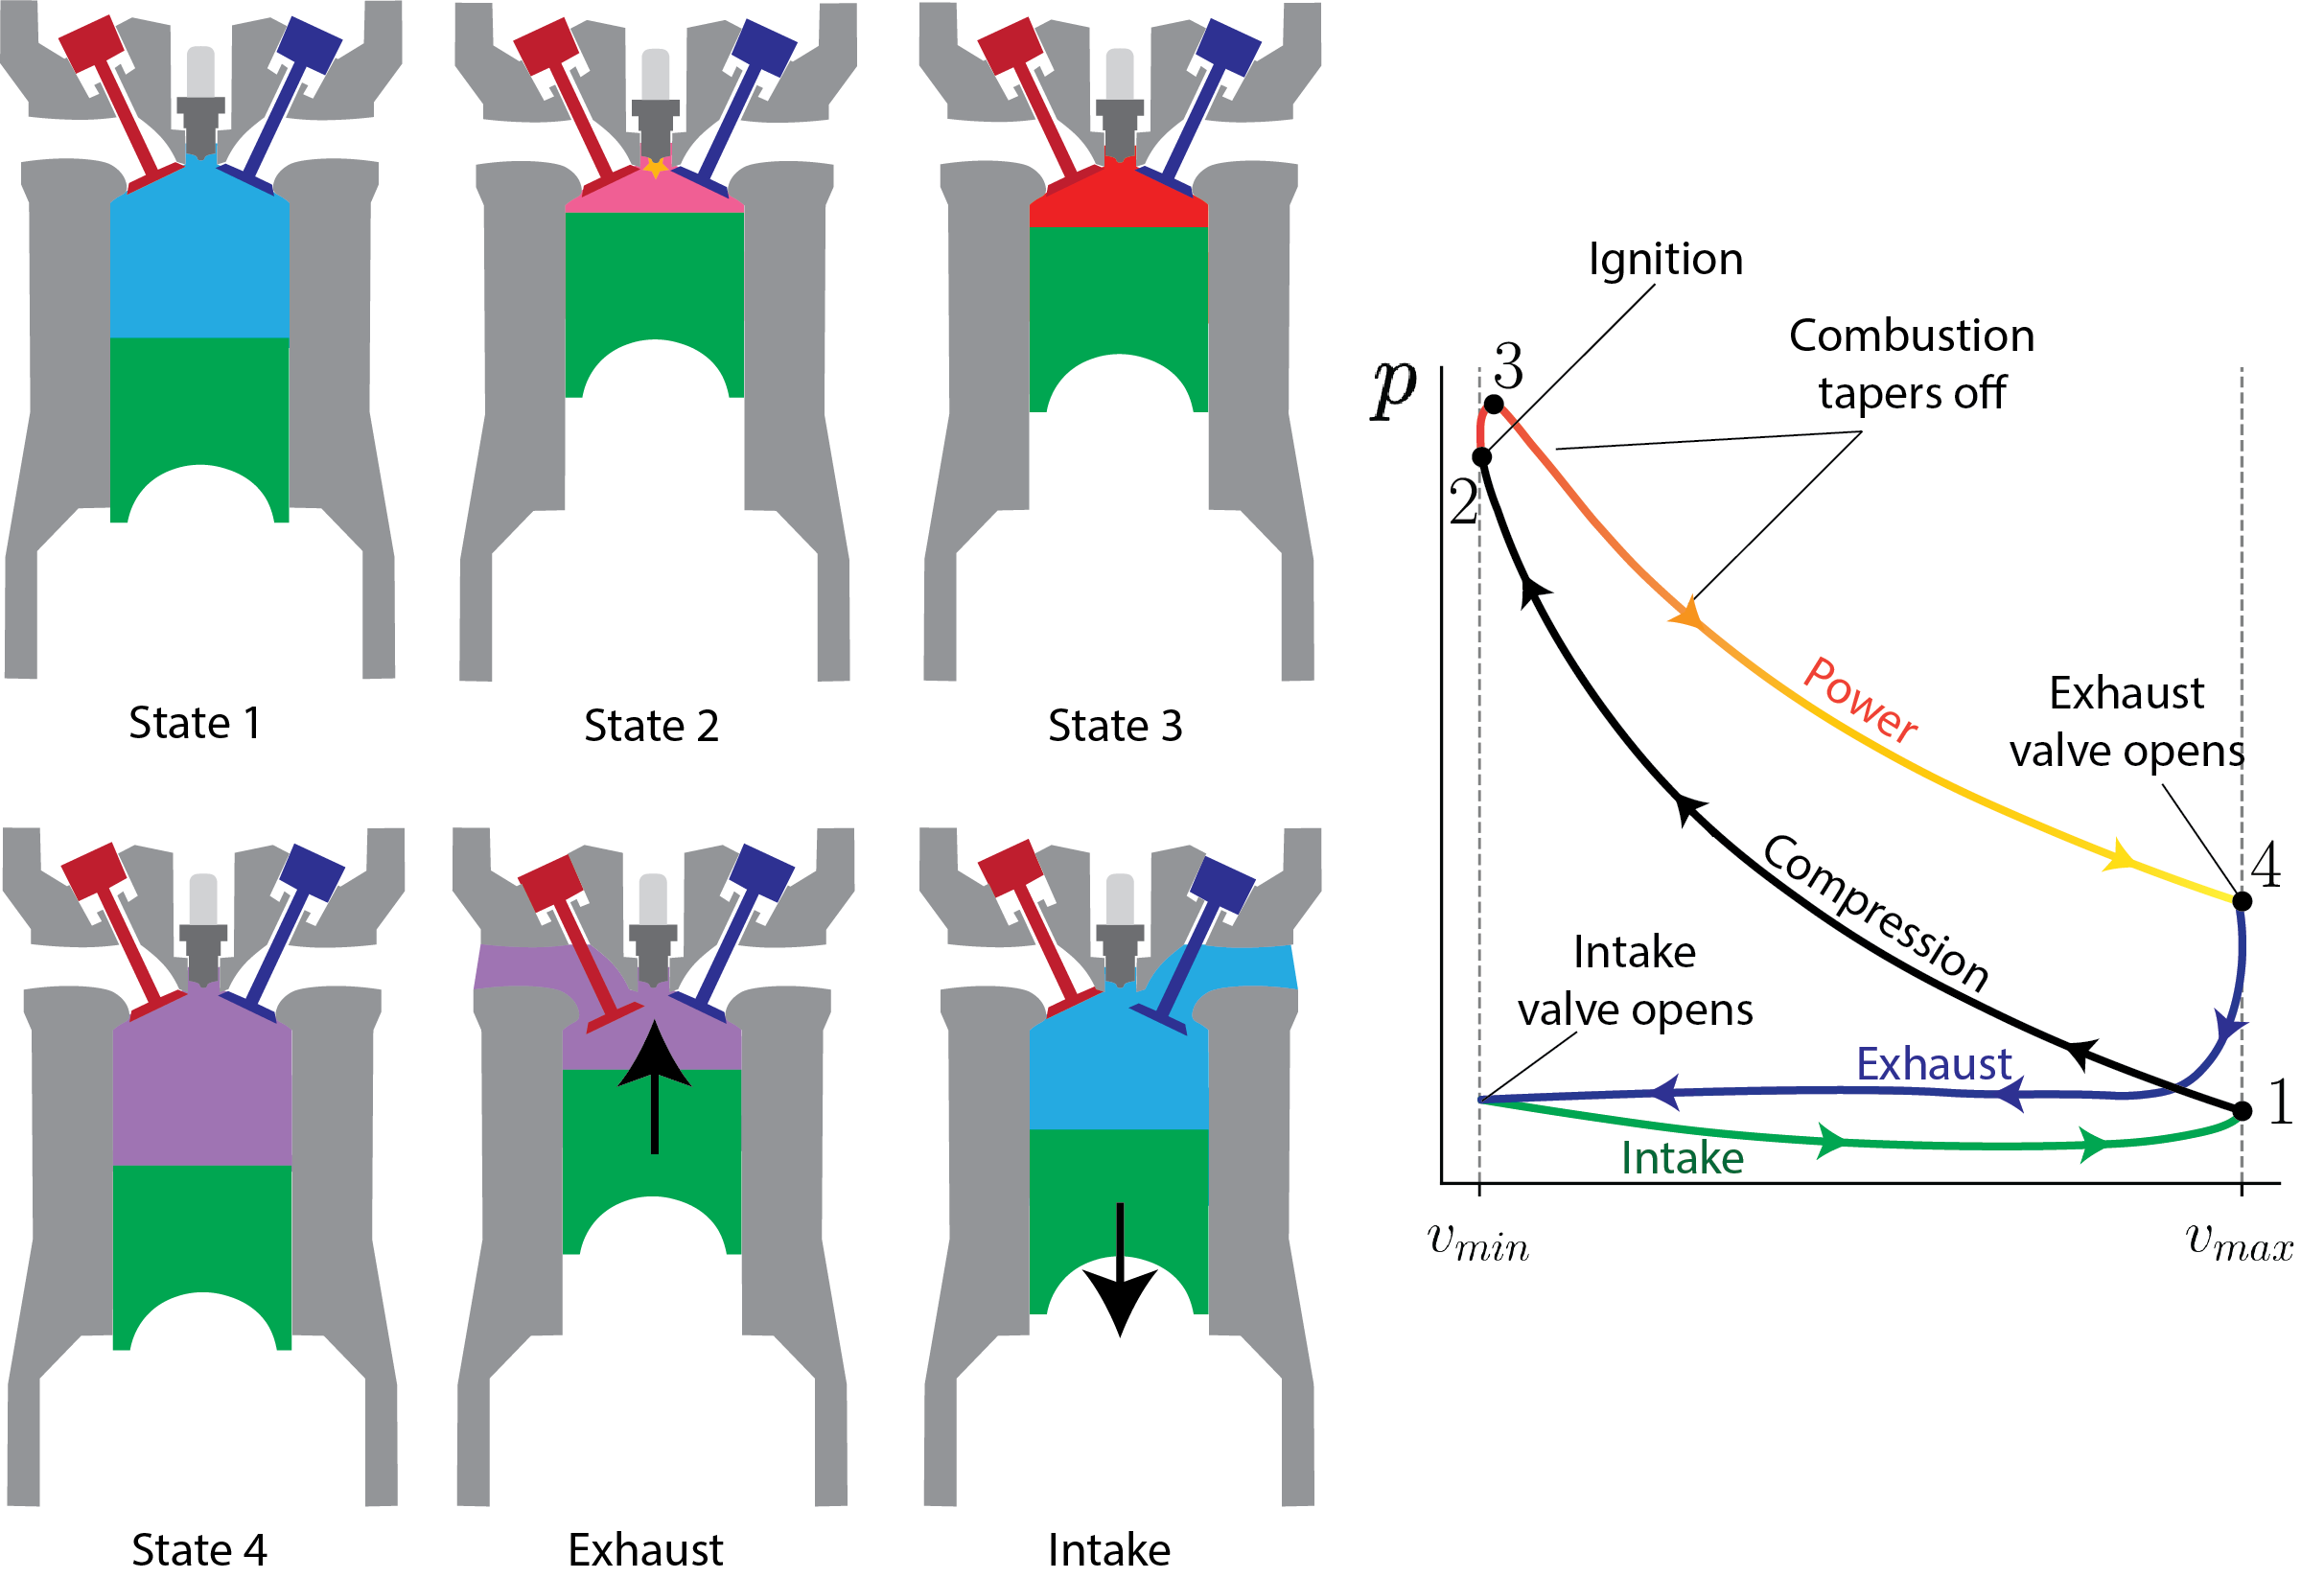
\includegraphics[width=0.9\textwidth]{FourStrokeCycle}
\caption{States of the four-stroke Otto Cycle with $p$-$v$ diagram.}
\label{fig:ch3_fourStroke}
\end{figure}

Figure \ref{fig:ch3_fourStroke} gives an approximate picture of an actual four-stroke spark-ignition cycle. It is extremely complex, both due to the gradual release of heat after ignition, as well as the mass transfer that occurs as the exhaust and intake valves open and close.  A perfect representation also needs to deal with the chemistry of combustion, the dynamics of fuel mixing, and the timing of various parts of the cycle.

Because the actual spark-ignition cycle is so complex, we make a number of simplifying assumptions.  First off, we use an ideal "air-standard" assumption, in which the working fluid is a fixed mass of air undergoing the complete cycle.  This simplification removes both the need for the exhaust/intake strokes and the need to consider the chemistry of combustion.  Instead of ignition, we use instantaneous heat addition between states 2 and 3.  Finally, the exhaust and intake strokes are replace by heat rejection between states 4 and 1.

\begin{figure}[H]
\centering
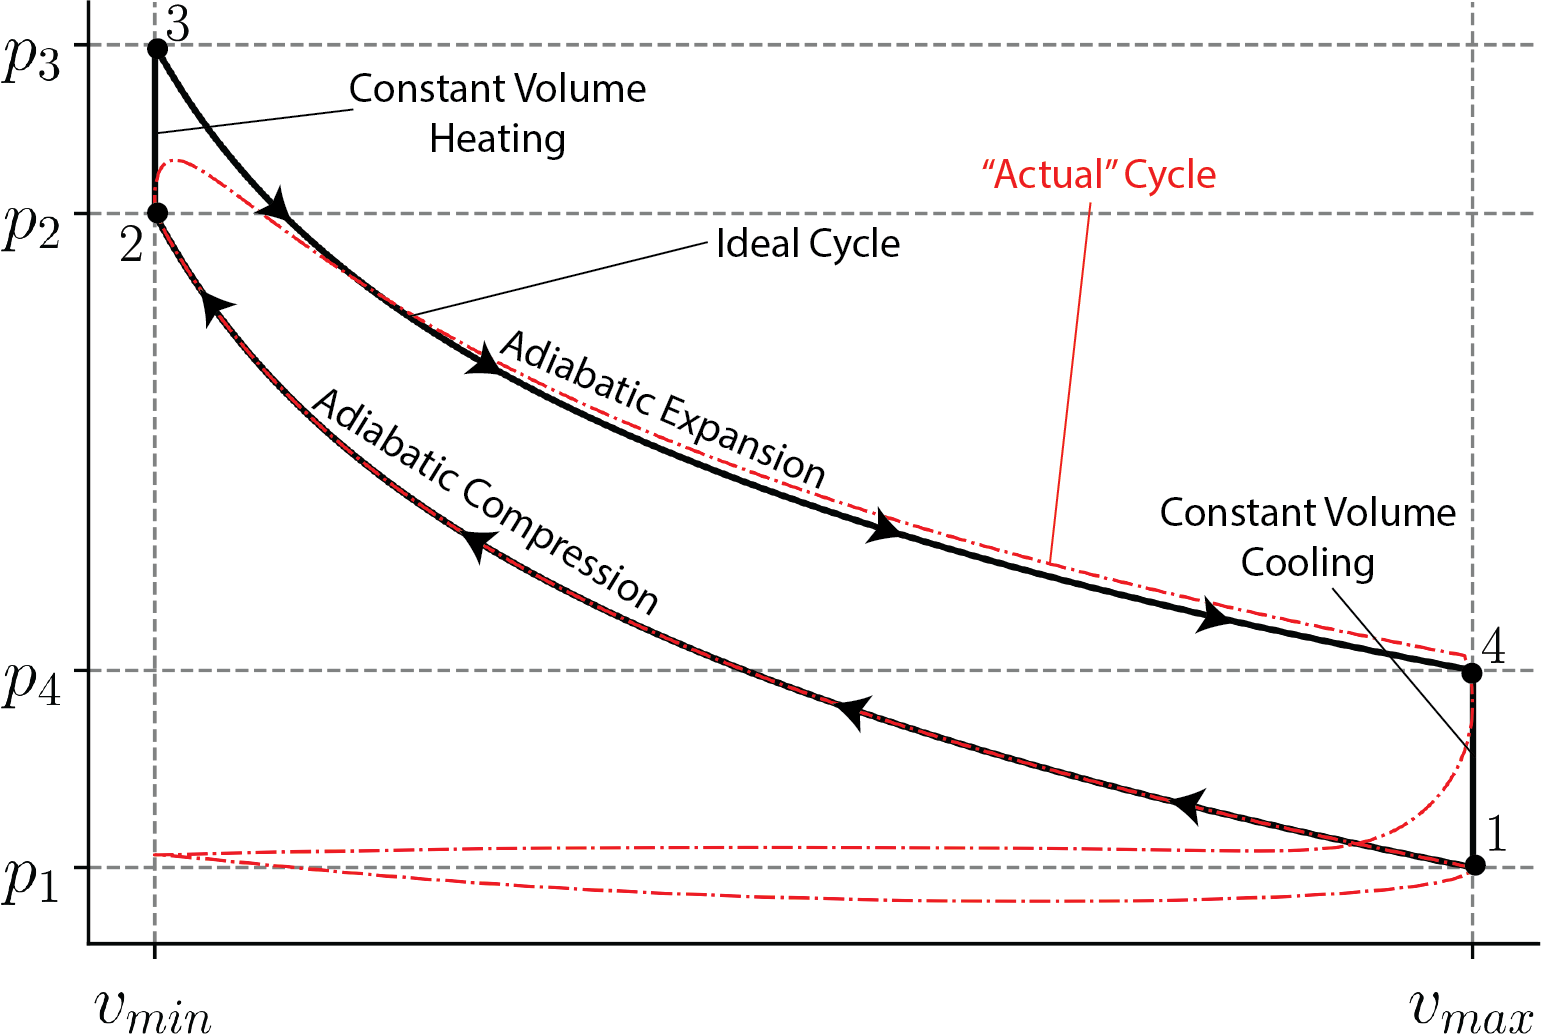
\includegraphics[width=0.75\textwidth]{OttoIdealCycle}
\caption{Ideal Otto cycle $p$-$v$ diagram compared to a simulated Otto cycle.}
\label{fig:ch3_ottoCycle}
\end{figure}

The end result is the cycle shown in Figure \ref{fig:ch3_ottoCycle}.  This looks very similar to the Stirling Cycle discussed in Section \ref{sec:ch3_stirling}.  The major difference between the two is that the compression between states 1 and 2 and the expansion between states 3 and 4 are both {\bf adiabatic}, rather than isothermal.  Analysis of these processes depends on the analysis done in Section \label{sec:ch3_idealGasAdiabatic}.

Note that the ideal cycle in Figure \ref{fig:ch3_ottoCycle} reaches significantly higher pressures than the actual cycle.  Additionally, the pressure at state 4 is slightly lower in the ideal cycle.  Both of these occur because of the assumption of instantaneous heat addition in the ideal cycle.  The actual cycle never reaches the high temperatures because expansion happens at the same time as heating, and the temperature is higher at state 4 because heat is added at a lower temperature, which means the air has a lower $c_v$ value.

The omission of the exhaust and intake strokes results in better efficiency for the ideal cycle, as work is required to both push out extra combustion products and to suck in fresh air. 
% --------------------------------------------------------------------
\subsection{Otto Cycle Analysis}

The Otto Cycle looks very similar to the Stirling Cycle discussed in Section \ref{sec:ch3_stirling}, with the key difference that the expansion and compression are adiabatic (no heat transfer) instead of isothermal.

The results of this can be seen in Table \ref{tab:ch3_otto}.  $\Delta u$ is always $c_v \Delta T$, though the definition of $\Delta T$ changes for each process.  For processes 1-2 and 3-4, $q=0$ because the processes are adiabatic.  For processes 2-3 and 4-1, $w=0$ because no work can be developed in a constant volume process.  The First Law ($\Delta u = q - w$) is used to fill in the remaining blanks.

\begin{table}[H]
  \centering
\def\arraystretch{1.5}
\caption{Tabular Representation of Energy Equation for the Otto Cycle}
\label{tab:ch3_otto}
\begin{tabular}{r|ccc}
            & $\Delta u$        & $q$             & $w$           \\ \hline
Process 1-2 & $ c_v (T_2-T_1)$ & 0                 &  $ -c_v (T_2-T_1)$ \\
Process 2-3 & $ c_v (T_3-T_2)$ & $ c_v (T_3-T_2)$   & 0       \\
Process 3-4 & $ c_v (T_4-T_3)$ & 0                 &  $ -c_v (T_4-T_3)$ \\ 
Process 4-1 & $ c_v (T_1-T_4)$ & $ c_v (T_1-T_4)$  &  0          \\ \hhline{=|===}
Total (net) & 0                 & $c_v (T_1-T_2+T_3-T_4)$ & $c_v (T_1-T_2+T_3-T_4)$
\end{tabular}
\def\arraystretch{1.0}
\end{table}

We are often interested in the {\bf thermal efficiency} of an engine, which is defined as $\eta_{th} = q_{in}/w_{net}$ in Equation \ref{eq:ch3_StirlingEfficiency}.  For the Otto engine, this becomes:
\begin{equation*}
  \eta_{th} = \frac{\cancel{c_v} \left(T_1-T_2+T_3-T_4\right)}{ \cancel{c_v} \left(T_3-T_2\right)} = 1 + \frac{T_1 - T_4}{T_3 - T_2}
\end{equation*}

Now we define the {\bf compression ratio}, $r$:
\begin{equation} \label{eq:ch3_comprat}
  r = \frac{v_{max}}{v_{min}}
\end{equation}
We can recognize that $v_{max}=v_1=v_4$ and $v_{min}=v_2=v_3$ to say that $r=v_1/v_2=v_4/v_3$.

We can then use the adiabatic relation for $T$ and $v$ from Equation \ref{eq:ch3_adiabaticTv} to make the following definitions:
\begin{align*}
  T_2 &= T_1 (v_2/v_1)^{-(\gamma-1)} = T_1 r^{\gamma-1}\\
  T_3 &= T_4 (v_3/v_4)^{-(\gamma-1)} = T_4 r^{\gamma-1}
\end{align*}

Using this, we can simplify the efficiency as follows:
\begin{align}
  \nonumber \eta_{th} &= 1 + \frac{ T_1-T_4}{ T_4 r^{\gamma-1} -T_1 r^{\gamma-1}} \\
  \nonumber \eta_{th} &= 1-\cancel{\frac{\left(T_4 - T_1\right)}{\left(T_4 - T_1\right)}} \frac{1}{r^{\gamma-1}} \\
  \label{eq:ch3_ottoeff} \eta_{th} &= 1 - \frac{1}{r^{\gamma-1}}
\end{align}

Equation \ref{eq:ch3_ottoeff} shows that the thermal efficiency is a function only of the compression ratio, $r$, and the ratio of specific heats, $\gamma$.  This simplified analysis requires the assumption that $\gamma$ is a constant over the entire cycle.  As long as $\gamma$ is chosen at or near $T_{avg}=\frac{1}{2}\left(T_{max}+T_{min}\right)$, this is a very reasonable assumption.

Example \ref{ex:ch3_otto} provides a closer look at an ideal Otto cycle.
\newpage
\begin{example}[label=ex:ch3_otto]{Otto Cycle}
  An ideal air-standard Otto cycle engine has a compression ratio of 8. At the beginning of the compression process, the working fluid is at 100 kPa, 27°C (300 K), and 800 kJ/kg heat is supplied during the constant volume heat addition process. Neatly sketch the pressure-volume [$p$-$v$] diagram for this cycle, and using the specific heat values for air at a typical average cycle temperature of 900 K determine:
\begin{enumerate}[a)]
\item the temperature and pressure of the air at the end of each process
\item the net work output/cycle [kJ/kg], and
\item the thermal efficiency [$\eta_{th}$] of this engine cycle.
\end{enumerate}

The first step is to draw the $p$-$v$ diagram of the complete cycle, including all the relevant information. We notice that neither volume nor mass have been provided, hence the diagram and solution will be in terms of specific quantities.

\begin{center}
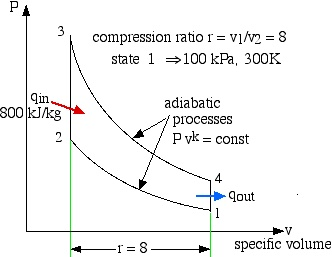
\includegraphics[width=0.65\textwidth]{OttoPV}
%\captionof{figure}{}
%\label{fig:ch2_example1}
\end{center}

We assume that the fuel-air mixture is represented by pure air. The relevant equations of state, internal energy and adiabatic process for air follow:
\begin{align*}
  pv&=RT & R &= 0.287 \frac{\rm kJ}{\rm kg\ K}\\
  \Delta u &= c_v \Delta T \\
  \frac{p_2}{p_1} &= \left(\frac{v_1}{v_2}\right)^{\gamma} & \frac{T_2}{T_1} &= \left(\frac{v_1}{v_2}\right)^{\gamma -1}
\end{align*}

Note that values for $c_v$ and $\gamma$ should come from the average value of temperature.  We won't know what the actual average temperature is until we solve the problem, but we are asked to use the ``typical average cycle temperature'' of 900 K.  We get this from the table of Specific Heat Capacities of Air.

\begin{equation*}
  c_{v,900\rm\ K} = 0.834 \frac{\rm kJ}{\rm kg\ K} \quad\quad\quad \gamma_{900\rm\ K} = 1.344
\end{equation*}

Compare these values to the nominal specific heat capacity values used for air at 300K: $C_v$ = 0.717 kJ/kg K and $\gamma$ = 1.4, and you will see the importance of using the Ideal Gas Tables.

We now go through all four processes in order to determine the temperature and pressure at the end of each process, as well as the work done and heat transferred during each process.

{\bf Process 1-2 - Adiabatic Compression:}
\begin{equation*}
  p_1 = 100\ {\rm kPa}, \quad \quad T_1 = 300\ {\rm K}
\end{equation*}
Starting at state 1, we compress the fluid adiabatically with a compression ratio of 8.  Keep in mind that the specific volume of state 1 will be {\bf larger} than that of state 2.
\begin{align*}
  &{\rm \bf Adiabatic} &\rightarrow& \redbox{q_{12} = 0\ \frac{\rm kJ}{\rm kg}} \\
  r &= \frac{v_1}{v_2} = 8 \\
  \frac{T_2}{T_1} &= \left(\frac{v_1}{v_2}\right)^{\gamma -1} = 8^{0.344} = 2.045 &\rightarrow & \redbox{T_2 = 613\ {\rm K}} \\
  \frac{p_2}{p_1} &= \left(\frac{v_1}{v_2}\right)^{\gamma} = 8^{1.344} = 16.359 &\rightarrow& \redbox{ p_2 = 1635\ {\rm kPa}}\\
\Delta u_{12} &= c_v \Delta T_{12} = \cancelto{0}{q_{12}} - w_{12} &\rightarrow& \redbox{w_{12} = -261\ \frac{\rm kJ}{\rm kg}}
\end{align*}

Note that we could also find the work through $\int p\: dv$.  The above approach is much simpler.

{\bf Process 2-3 - Constant Volume Combustion:}
From state 2, we add heat at constant volume ($v_3 = v_2$).
\begin{align*}
  &{\rm \bf Constant\ Volume} &\rightarrow& \redbox{w_{23} = 0\ \frac{\rm kJ}{\rm kg}} \\
   &{\rm \bf Given} &\rightarrow& \redbox{q_{23} = 800\ \frac{\rm kJ}{\rm kg}} \\
  q = c_v \Delta T \quad&\rightarrow\quad T_3 - T_2 = \frac{q}{c_v} \\
  T_3 - T_2 &= \frac{800\ \rm kJ/kg}{0.834\ \rm kJ/kgK} &\rightarrow &\redbox{T_3 = 1572 \ {\rm K}}\\
  \frac{p_3 }{p_2 } \frac{\cancel{v_3}}{\cancel{v_2}}&= \frac{\cancel{R}}{\cancel{R}}\frac{T_3}{T_2} &\rightarrow &\redbox{p_3 = 4193\ {\rm kPa}}
\end{align*}
\newpage
{\bf Process 3-4 - Adiabatic Expansion:}
From state 3 to 4, we again use the compression ratio, but recognize that $v_4 > v_3$.
\begin{align*}
  &{\rm \bf Adiabatic} &\rightarrow& \redbox{q_{34} = 0\ \frac{\rm kJ}{\rm kg}} \\
  r &= \frac{v_3}{v_4} = \frac{1}{8} \\
  \frac{T_4}{T_3} &= \left(\frac{v_3}{v_4}\right)^{\gamma -1} = \frac{1}{8}^{0.344} = 0.489 &\rightarrow &\redbox{T_3 = 769\ {\rm K}} \\
  \frac{p_4}{p_3} &= \left(\frac{v_3}{v_4}\right)^{\gamma} = \frac{1}{8}^{1.344} = 0.0611 &\rightarrow &\redbox{p_4 = 256\ {\rm kPa}} \\
  \Delta u_{12} &= c_v \Delta T_{12} = \cancelto{0}{q_{12}} - w_{12} &\rightarrow& \redbox{w_{34} = 670\ \frac{\rm kJ}{\rm kg}}
\end{align*}

{\bf Process 4-1 - Constant Volume Heat Rejection:}
From state 4, we reject heat at constant volume ($v_1 = v_4$).
\begin{align*}
  &{\rm \bf Constant\ Volume} &\rightarrow& \redbox{w_{23} = 0\ \frac{\rm kJ}{\rm kg}} \\
  \Delta u_{41} &= c_v \Delta T_{41} = q_{41} - \cancelto{0}{w_{12}} &\rightarrow& \redbox{q_{41} = -391\ \frac{\rm kJ}{\rm kg}}
\end{align*}

{\bf Cycle Summary:} Now we can build a summary of the processes using Table \ref{tab:ch3_otto}.
\begin{table}[H]
  \centering
\def\arraystretch{1.5}
%\caption{Tabular Representation of Energy Equation for Otto Cycle}
%\label{tab:ch3_stirling}
\begin{tabular}{r|ccc}
            & $\Delta U$        & $Q$      &$W$     \\ \hline
Process 1-2 & -261 kJ/kg        & 0 &  -261 kJ/kg  \\
Process 2-3 & 800 kJ/kg   & 800 kJ/kg & 0               \\
Process 3-4 & 670 kJ/kg   & 0              &  670 kJ/kg \\ 
Process 4-1 & -391 kJ/kg   &  -391 kJ/kg &  0  \\ \hhline{=|===}
Total (net) & 0                 &  409 kJ/kg & 409 kJ/kg
\end{tabular}
\def\arraystretch{1.0}
\end{table}

The net work created by a single cycle was 409 kJ/kg, and the heat added per cycle was 800 kJ/kg.  We can find the thermal efficiency as follows:
\begin{align*}
  \eta_{th} &= \frac{w_{net}}{q_{in}} = \frac{409\ {\rm kJ/kg}}{800\ {\rm kJ/kg}} &\rightarrow& \redbox{\eta_{th} = 51\%}
\end{align*}

Note that using constant specific heat values over the cycle we can determine the thermal efficiency directly from the ratio of specific heat capacities $\gamma$ and the compression ratio $r$ using Equation \ref{eq:ch3_ottoeff}:
\begin{equation*} 
  \eta_{th} = 1 - \frac{1}{r^{\gamma-1}} = 1 - \frac{1}{8^{0.344}}= 0.511
\end{equation*}
This matches closely with the analysis above.

\end{example}



% --------------------------------------------------------------------
\section{Air-Standard Diesel Cycle}
% --------------------------------------------------------------------

The Air Standard Diesel cycle is the ideal cycle for Spark-Ignition (CI) reciprocating engines, first proposed by Rudolph Diesel over 100 years ago. The following link by the Kruse Technology Partnership describes the \href{http://www.kruse-ltc.com/diesel.php}{four-stroke diesel cycle} operation including a short history of Rudolf Diesel. The four-stroke diesel engine is usually used in motor vehicle systems, whereas larger marine systems usually use the \href{https://auto.howstuffworks.com/diesel-two-stroke1.htm}{two-stroke diesel cycle}. Once again we have an excellent animation produced by Matt Keveney presenting the operation of the \href{http://animatedengines.com/diesel.html}{four-stroke diesel cycle}.

The analysis of the Diesel cycle is very similar to that of the Otto cycle which we analyzed in the previous section. We will use the ideal "air-standard" assumption in our analysis. Thus the working fluid is a fixed mass of air undergoing the complete cycle which is treated throughout as an ideal gas. All processes are ideal, combustion is replaced by heat addition to the air, and exhaust is replaced by a heat rejection process which restores the air to the initial state.

\begin{figure}[H]
\centering
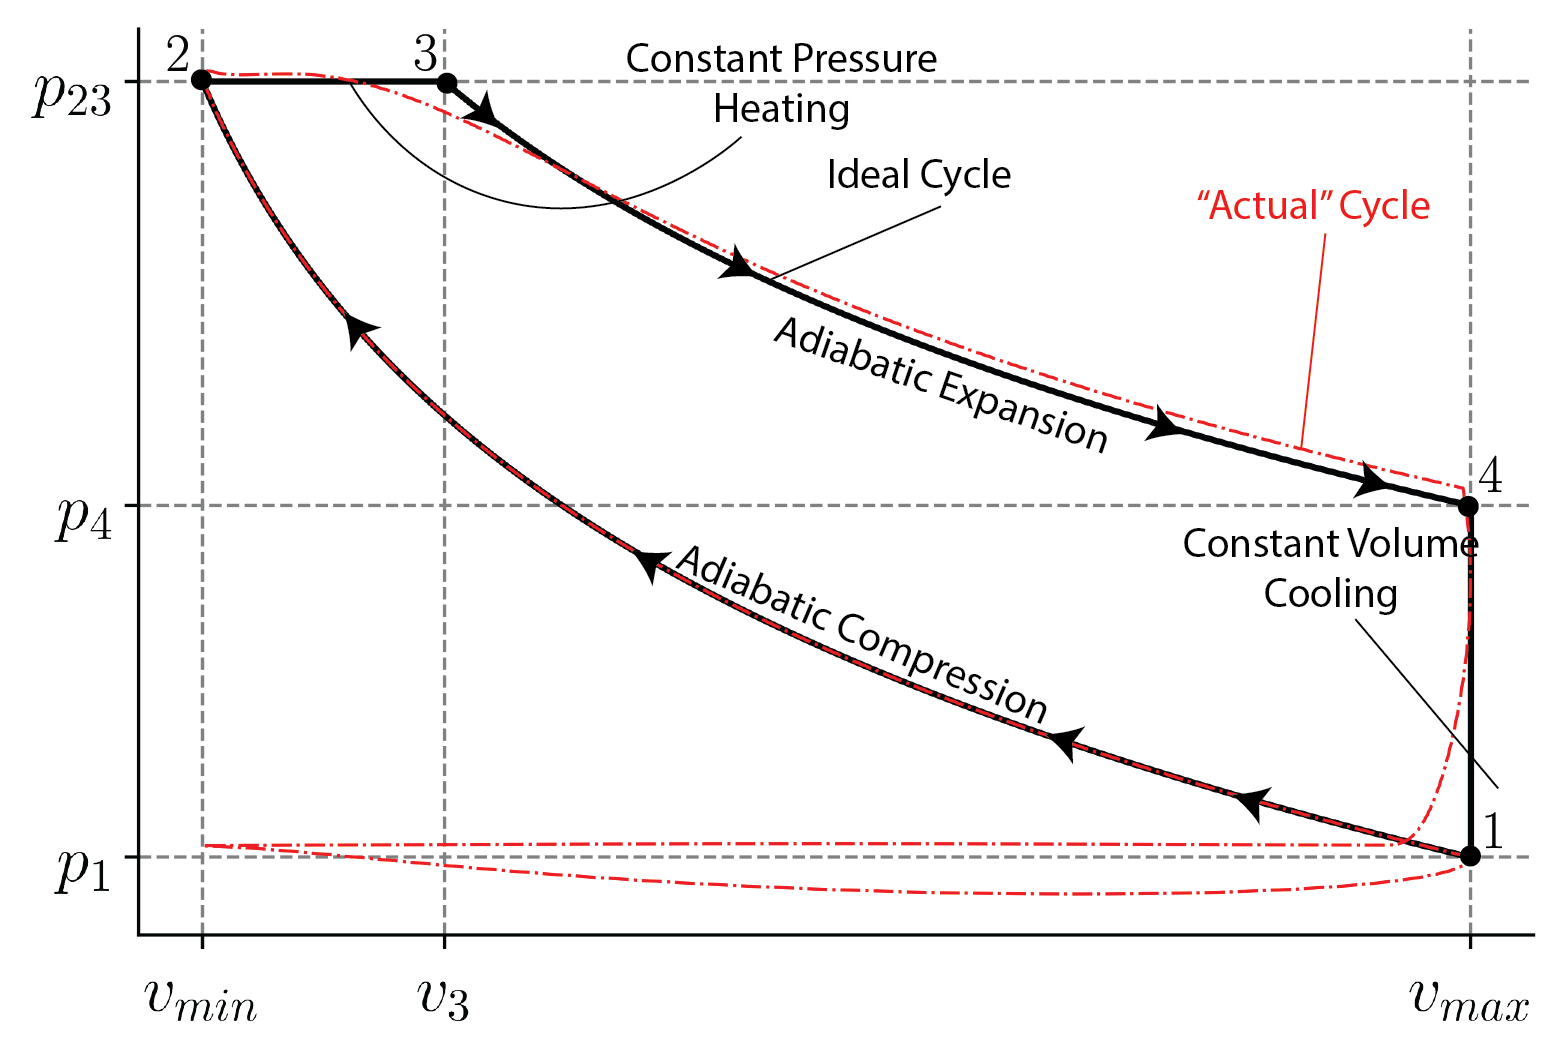
\includegraphics[width=0.75\textwidth]{DieselIdealCycle}
\caption{Ideal Diesel Cycle $p$-$v$ diagram compared to a simulated Diesel Cycle.}
\label{fig:ch3_dieselCycle}
\end{figure}

The most significant difference between the ideal Otto cycle and the ideal Diesel cycle is the method of igniting the fuel-air mixture.  For the Otto cycle, spark-ignition allows us to maintain a relatively low compression ratio (around 8:1), and time the combustion such that it results in a sudden jump in pressure while the volume remains essentially constant.

In contrast, in order to self-ignite, the ideal Diesel cycle needs an extremely high compression ratio (around 18:1) to allow the air to reach the ignition temperature of the fuel. Only then is the fuel injected.  The timing of ignition is such that combustion adds heat as the piston is in the process of expanding, which leads to combustion at nearly a constant pressure, as seen in Figure \ref{fig:ch3_dieselCycle}.

After combustion, the rest of the cycle (expansion and exhaust) is essentially identical to that of the ideal Otto cycle.

\subsection{Diesel Cycle Analysis}

The Diesel cycle is very similar to the Otto cycle, with the major change that heating occurs at constant pressure, rather than constant volume.  The major complication is that work occurs at the same time as heat transfer, unlike in the Otto cycle, where work and heat transfer are perfectly decoupled.

\begin{table}[H]
  \centering
\def\arraystretch{1.5}
\caption{Tabular Representation of Energy Equation for the Diesel Cycle}
\label{tab:ch3_diesel}
\begin{tabular}{r|ccc}
            & $\Delta u$        & $q$             & $w$           \\ \hline
Process 1-2 & $ c_v (T_2-T_1)$ & 0                 &  $ -c_v (T_2-T_1)$ \\
Process 2-3 & $ c_v (T_3-T_2)$ & $ c_p (T_3-T_2)$   & $p_{23} (v_3 - v_2) = R(T_3-T_2)$ \\
Process 3-4 & $ c_v (T_4-T_3)$ & 0                 &  $ -c_v (T_4-T_3)$ \\ 
Process 4-1 & $ c_v (T_1-T_4)$ & $ c_v (T_1-T_4)$  &  0          \\ \hhline{=|===}
Total (net) & 0                 & $c_v (T_1-T_4)+c_p(T_3-T_2)$ & $c_v (T_1-T_4) + c_p(T_3-T_2)$
\end{tabular}
\def\arraystretch{1.0}
\end{table}

Let's again find the thermal efficiency:
\begin{equation*}
  \eta_{th} = \frac{c_v \left(T_1-T_4\right)+c_p\left(T_3-T_2\right)}{ c_p \left(T_3-T_2\right)} = 1-\frac{\left(T_4-T_1\right)}{\gamma \left(T_3-T_2\right)}
\end{equation*}

Often, rather than indicating the amount of heat from combustion, the heat addition process is defined by a {\bf cutoff ratio}.  This is another volume ratio, defined as:
\begin{equation} \label{eq:ch3_cutoffRatio}
  r_c = \frac{v_3}{v_2}
\end{equation}

The cutoff ratio will always be less than the compression ratio (Equation \ref{eq:ch3_compressionRatio}).  Additionally, this ratio allows us to link each of our temperatures using $r$, $r_c$, and $\gamma$:
\begin{align*}
  T_2 &= T_1\: r^{\gamma-1}  &\quad& \text{from adiabatic relations}\\
  T_3 &= T_2\: r_c &\quad& \text{from the ideal gas law}\\
  T_4 &= T_3 \left(\frac{r_c}{r}\right)^{\gamma-1} &\quad& \text{from adiabatic relations}
\end{align*}

We can simplify $T_3$ and $T_4$ as follows:
\begin{align*}
  T_3 &= T_1\: r^{\gamma-1}\: r_c \\
  T_4 &= T_1\: \cancel{r^{\gamma-1}}\: r_c \left(\frac{r_c}{\cancel{r}}\right)^{\gamma-1} = T_1 r_c r_c^{\gamma-1} = T_1 r_c^{\gamma}
\end{align*}

Substituting the above relationships into the thermal efficiency gives us the following:
\begin{align}
  \nonumber \eta_{th} &= 1 - \frac{T_1 r_c^{\gamma} - T_1}{\gamma \left(T_1 \: r^{\gamma-1}\: r_c -  T_1\: r^{\gamma-1}\right)} \\
  \label{eq:ch3_dieseleff} \eta_{th} &= 1 - \frac{1}{\gamma\:r^{\gamma-1}}\frac{r_c^{\gamma} - 1}{r_c -  1}
\end{align}

As $r_c\rightarrow 1$, Equation \ref{eq:ch3_dieseleff} approaches Equation \ref{eq:ch3_ottoeff}, the Otto efficiency.

Example \ref{ex:ch3_diesel} provides a closer look at an ideal Diesel cycle.

\begin{example}[label=ex:ch3_diesel]{Diesel Cycle}
  An ideal air-standard Diesel cycle engine has a compression ratio of 18 and a cutoff ratio of 2. At the beginning of the compression process, the working fluid is at \mbox{100 kPa}, 27°C (300 K).
\begin{enumerate}[a)]
\item Determine the temperature and pressure of the air at the end of each process.
\item Determine the net work output per cycle [kJ/kg].
\item Determine the thermal efficiency.
\end{enumerate}

The first step is to draw a diagram representing the problem, including all the relevant information. We notice that neither volume nor mass is given, hence the diagram and solution will be in terms of specific quantities. The most useful diagram for a heat engine is the $p$-$v$ diagram of the complete cycle:

\begin{center}
\includegraphics[width=0.75\textwidth]{DieselPV}
%\captionof{figure}{}
%\label{fig:ch2_example1}
\end{center}

In order to use constant specific heats, we must guess the average temperature of the cycle.  For this analysis, we will use 900 K to calculate the specific heats.  We will then check that value at the end of the analysis.

\begin{equation*}
  c_{p,900\rm\ K} = 1.121\ \frac{\rm kJ}{\rm kg\ K} \quad\quad\quad \gamma_{900\rm\ K} = 1.344
\end{equation*}

We now go through all four processes in order to determine the temperature and pressure at the end of each process, as well as the work done and heat transferred during each process.

{\bf Process 1-2 - Adiabatic Compression:}
\begin{equation*}
  p_1 = 100\ {\rm kPa}, \quad \quad T_1 = 300\ {\rm K}
\end{equation*}
Starting at state 1, we compress the fluid adiabatically with a compression ratio of 18.  Keep in mind that the specific volume of state 1 will be {\bf larger} than that of state 2.
\begin{align*}
  &{\rm \bf Adiabatic} &\rightarrow& \redbox{q_{12} = 0\ \frac{\rm kJ}{\rm kg}} \\
  r &= \frac{v_1}{v_2} = 18 \\
  \frac{T_2}{T_1} &= \left(\frac{v_1}{v_2}\right)^{\gamma -1} = 18^{0.344} = 2.703 &\rightarrow & \redbox{T_2 = 811\ {\rm K}} \\
  \frac{p_2}{p_1} &= \left(\frac{v_1}{v_2}\right)^{\gamma} = 18^{1.344} = 48.650 &\rightarrow& \redbox{ p_2 = 4865\ {\rm kPa}}%\\
%\Delta u_{12} &= c_v \Delta T_{12} = \cancelto{0}{q_{12}} - w_{12} &\rightarrow& \redbox{w_{12} = -261 \frac{\rm kJ}{\rm kg}}
\end{align*}

{\bf Process 2-3 - Constant Pressure Combustion:}
From state 2, we add heat at constant pressure ($p_3 = p_2$), with a cutoff ratio of 2.
\begin{align*}
  &{\rm \bf Constant\ Pressure}  &\rightarrow& \redbox{p_3 = 4865\ {\rm kPa}} \\
  \frac{\cancel{p_3}}{\cancel{p_2} } \cancelto{2}{\frac{v_3}{v_2}}&= \frac{\cancel{R}}{\cancel{R}}\frac{T_3}{T_2} &\rightarrow &\redbox{T_3 = 1622\ {\rm K}}
\end{align*}
For this process, both work and heat transfer are present.  However, we can find the heat transfer by using the constant pressure specific heat, $c_p$:
\begin{align*}
    q_{23} = c_p (T_3 - T_2) =1.121\ \frac{\rm kJ}{\rm kg\ K} \cdot \left(1622\ {\rm K} - 811\ {\rm K}\right)\quad&\rightarrow& \redbox{q_{23} = 909\ \frac{\rm kJ}{\rm kg}}
\end{align*}

{\bf Process 3-4 - Adiabatic Expansion:}
To calculate the volume ratio between states 3 and 4, we simply divide the compression ratio by the cutoff ratio:
\begin{equation*}
  \frac{v_4}{v_3} = \frac{v_1}{v_3} = \frac{v_2}{v_3}\frac{v_1}{v_2} = \frac{r}{r_c}
\end{equation*}
This allows us to follow a similar pattern to Process 1-2.
\begin{align*}
  &{\rm \bf Adiabatic} &\rightarrow& \redbox{q_{34} = 0\ \frac{\rm kJ}{\rm kg}} \\
  \frac{v_3}{v_4} = \frac{r_c}{r}=\frac{1}{9} \\
  \frac{T_4}{T_3} &= \left(\frac{v_3}{v_4}\right)^{\gamma -1} = \frac{1}{9}^{0.344} = 0.470 &\rightarrow &\redbox{T_3 = 762\ {\rm K}} \\
  \frac{p_4}{p_3} &= \left(\frac{v_3}{v_4}\right)^{\gamma} = \frac{1}{8}^{1.344} = 0.0522 &\rightarrow &\redbox{p_4 = 254\ {\rm kPa}}
\end{align*}

{\bf Process 4-1 - Constant Volume Heat Rejection:}
From state 4, we reject heat at constant volume ($v_1 = v_4$).
\begin{align*}
  \Delta u_{41} &= c_v \Delta T_{41} = q_{41} - \cancelto{0}{w_{12}} &\rightarrow& \redbox{q_{41} = -385\ \frac{\rm kJ}{\rm kg}}
\end{align*}

{\bf Cycle Summary:} Notice that we didn't calculate the work for any of the processes.  The reason for this is we can more easily obtain the net work, $w_{net}$, by finding the net heat transfer, $q_{net}$.  For a cycle, the net work and the net heat transfer will be equal.
\begin{equation*}
  w_{net} = q_{net} = 909\ \frac{\rm kJ}{\rm kg} - 385\ \frac{\rm kJ}{\rm kg} \quad \rightarrow \quad \redbox{w_{net} = 524\ \frac{\rm kJ}{\rm kg}}
\end{equation*}

We can find the thermal efficiency as follows:
\begin{align*}
  \eta_{th} &= \frac{w_{net}}{q_{in}} = \frac{524\ {\rm kJ/kg}}{909\ {\rm kJ/kg}} &\rightarrow& \redbox{\eta_{th} = 58\%}
\end{align*}

As a side note, our maximum temperature was about 1600 K, so an average temperature of 900 K for finding $c_p$ and $\gamma$ is reasonable.

You may wonder at the unrealistically high thermal efficiency obtained in this example. In this idealized analysis we have ignored many loss effects that exist in practical heat engines. We will begin to understand some of these loss mechanisms when we study the Second Law in Chapter 5.
\end{example}

\section{Using Software: Plotting a Cycle in Python}
In Section \ref{sec:ch1_colab}, we introduced the various plotting options available in Python through \href{https://colab.research.google.com}{Google Colab}.  In Section \ref{sec:ch2_colab}, we used Colab in order to implement the ideal gas law.

In this section, we will combine the two in order to plot the Otto cycle in Python.

\subsection{Solving the Otto Cycle in Colab}
To start off, let's solve Example 3.5 in Colab.  We still need to start off by including our library imports:

\begin{Verbatim}[commandchars=\\\{\}]
\textcolor{OliveGreen}{# Clear all variable definitions}
\textcolor{blue}{\%reset} -f                         
\textcolor{violet}{from} numpy \textcolor{violet}{import} *               \textcolor{OliveGreen}{# Import common numerical functions (like sqrt)}
\textcolor{violet}{from} matplotlib.pyplot \textcolor{violet}{import} *   \textcolor{OliveGreen}{# Import plotting functions (like plot)}
\textcolor{violet}{import} CoolProp.CoolProp \textcolor{violet}{as} CP    \textcolor{OliveGreen}{# Import CoolProp library}
\end{Verbatim}

With those in place, we define the known values for this Otto cycle:
\begin{Verbatim}[commandchars=\\\{\}]
\textcolor{OliveGreen}{# Given Values}                
cv    = \textcolor{JungleGreen}{0.834}      \textcolor{OliveGreen}{# Constant volume specific heat for air at 900 K (kJ/kgK)}
gamma = \textcolor{JungleGreen}{1.344}      \textcolor{OliveGreen}{# Ratio of specific heats for air at 900 K (-)}
Rgas = \textcolor{JungleGreen}{8.314}/\textcolor{JungleGreen}{28.97} \textcolor{OliveGreen}{# Gas constant for air (kJ/kgK)}
r = \textcolor{JungleGreen}{8}              \textcolor{OliveGreen}{# Compression ratio of cycle (-)}
qin = \textcolor{JungleGreen}{800}          \textcolor{OliveGreen}{# Combustion heat transfer (kJ/kg)}
T1 = \textcolor{JungleGreen}{300}           \textcolor{OliveGreen}{# Initial temperature (K)}
p1 = \textcolor{JungleGreen}{100}           \textcolor{OliveGreen}{# Initial pressure (kPa)}
\end{Verbatim}

The compression ratio is our path to state 2, so we need to start off by finding the specific volume of state 1:

\begin{Verbatim}[commandchars=\\\{\}]
\textcolor{OliveGreen}{# Find v2}                
v1 = Rgas * T1 / p1  \textcolor{OliveGreen}{# Ideal Gas Law}
v2 = v1 / r          \textcolor{OliveGreen}{# compression ratio r = v1/v2}
\end{Verbatim}

The pressure and temperature of state 2 can be found using the adiabatic ideal gas equations (Equations \ref{eq:ch3_adiabaticIdealGasTV} and \ref{eq:ch3_adiabaticIdealGaspV}):

\begin{Verbatim}[commandchars=\\\{\}]
\textcolor{OliveGreen}{# Find p2 and T2 with adiabatic ideal gas equations}                
T2 = T1 * (v1/v2)**(gamma-1)
p2 = p1 * (v1/v2)**gamma  
\end{Verbatim}

The volume at state 3 is the same as at state 2.  The temperature at state 3 is found using the equation for constant-volume heat addition.  The pressure can be found through the ideal gas law.
\begin{Verbatim}[commandchars=\\\{\}]
\textcolor{OliveGreen}{# Find values of state 3 (constant volume heat addition)}                
v3 = v2             \textcolor{OliveGreen}{# constant volume process}
T3 = T2 + qin/cv    \textcolor{OliveGreen}{# q = cv*deltaT}
p3 = T3*Rgas/v3     \textcolor{OliveGreen}{# Ideal gas law}
\end{Verbatim}

The volume at state 4 is the same as state 1.  The temperature and pressure can be found through the adiabatic ideal gas law equations.

\begin{Verbatim}[commandchars=\\\{\}]
\textcolor{OliveGreen}{# Find p4 and T4 with adiabatic ideal gas equations}                
v4 = v1
T4 = T3 * (v3/v4)**(gamma-1)
p4 = p3 * (v3/v4)**gamma  
\end{Verbatim}

At this point, we have each of our four states fully defined.  If we want to know the values, we can use the print command:

\begin{Verbatim}[commandchars=\\\{\}]
\textcolor{OliveGreen}{# Output state values}                
print(\textcolor{purple}{'State    Pressure    Temperature    Spec. Volume'})
print(\textcolor{purple}{'  1     %9.3f    %9.3f    %9.3f'}% (p1, T1, v1))
print(\textcolor{purple}{'  2     %9.3f    %9.3f    %9.3f'}% (p2, T2, v2))
print(\textcolor{purple}{'  3     %9.3f    %9.3f    %9.3f'}% (p3, T3, v3))
print(\textcolor{purple}{'  4     %9.3f    %9.3f    %9.3f'}% (p4, T4, v4))
\end{Verbatim}

This set of commands gives us the following table:
\begin{verbatim}
State    Pressure    Temperature    Spec. Volume
  1       100.000      300.000        0.861
  2      1635.886      613.457        0.108
  3      4193.839     1572.690        0.108
  4       256.365      769.095        0.861
\end{verbatim}

This print command looks a lot different than what we've used in the past.  Instead of manually putting in each of the values we wanted to print, we used {\bf placeholders}, which were then filled after we completed the format.  This allows us to create a small table without having to spend a ton of time fidgeting with spacing.

The placeholders have three components:
\begin{itemize}
\item The first value (9) indicates how much total space to give the number.  A smaller number will provide less white space.  If the number requires more space than given, Python will automatically give as much as needed (which would mess up our table).
\item The second piece (.3) indicates the precision, or how many numbers after the decimal point will be included.
\item The final piece (f) is an argument or conversion specifier.  You may want to use \verb~%9.3e~ instead for very large or small numbers to use an exponential format (e.g. \verb~4.194e+03~ instead of \verb~4193.839~).
\end{itemize}

\subsection{Plotting the States}
With our states fully known, let's plot the properties on a $p$-$v$ diagram.

We only have four values, so we can create our list manually:

\begin{verbatim}
plot([v1, v2, v3, v4], [p1, p2, p3, p4])
\end{verbatim}

This results in the following plot:
\begin{center}
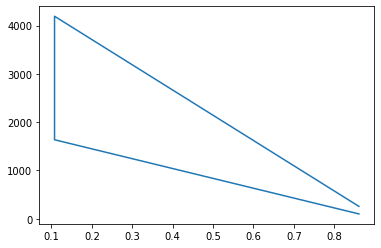
\includegraphics[width=0.6\textwidth]{initialPVDiagram}
%\captionof{figure}{}
%\label{fig:ch2_example1}
\end{center}

This plot has a number of issues.  We need labels and better limits for the axes, the cycle doesn't make a full circuit, and the adiabatic compression and expansion are straight lines, rather than following the path they should.
Additionally, it would be nice to label each of the states with a number.  Let's tackle each of these.
\subsection{Revising the Plot}
\subsubsection{Axis Labels and Limits}
We've done this before in Section \ref{sec:ch1_colab}, but to re-cap, we'll use the \verb~xlabel~, \verb~ylabel~, and \verb~axis~ commands.
\begin{Verbatim}[commandchars=\\\{\}]
xlabel(\textcolor{purple}{'Spec. Volume [m^3/kg]'})
ylabel(\textcolor{purple}{'Pressure [kPa]'})
axis([\textcolor{ForestGreen}{0}, \textcolor{ForestGreen}{1}, \textcolor{ForestGreen}{0}, \textcolor{ForestGreen}{4500}])
\end{Verbatim}

\subsubsection{Adiabatic Compression/Expansion Lines} \label{sec:plottingCurvedLines}
This one is a bit more difficult.  In order to create curved lines, we need to create an array to work with.  We know the limits of specific volume, so we'll use that as our base.
\begin{Verbatim}[commandchars=\\\{\}]
vArray = linspace(v2, v1, \textcolor{ForestGreen}{100})
\end{Verbatim}

Once we have that in hand, we want define our pressure array by substituting the volume array for $v_2$ in Equation \ref{eq:ch3_adiabaticIdealGaspV}.

\begin{Verbatim}[commandchars=\\\{\}]
pArrayComp = p1*(vArray/v1)**-gamma
\end{Verbatim}

We can do the exact same thing for the expansion stroke by substituting $p_1$ for $p_3$ and $v_1$ for $v_3$:
\begin{Verbatim}[commandchars=\\\{\}]
pArrayExp = p3*(vArray/v3)**-gamma
\end{Verbatim}

Let's add two plot commands to plot these two lines, making them both blue.
\begin{Verbatim}[commandchars=\\\{\}]
plot(vArray, pArrayComp, \textcolor{purple}{'b'})
plot(vArray, pArrayExp, \textcolor{purple}{'b'})
\end{Verbatim}

\subsubsection{Adding State Labels}

To label the states, we use matplotlib's \verb~text~ command:

\begin{Verbatim}[commandchars=\\\{\}]
text(v1+.01, p1-50, \textcolor{purple}{'1'})  \textcolor{OliveGreen}{# Place the text '1' next to state 1}
text(v2-.03, p2-50, \textcolor{purple}{'2'})
text(v3-.03, p3+50, \textcolor{purple}{'3'})
text(v4+.01, p4+50, \textcolor{purple}{'4'})
\end{Verbatim}

The first two arguments tell Colab where to place the text, and the third argument is what text to type.  This can be finicky, and the easiest way to determine correct placement is just to alter the values added or subtracted from the specific volume and pressure.

After all of the changes above, we end up with the following:
\begin{center}
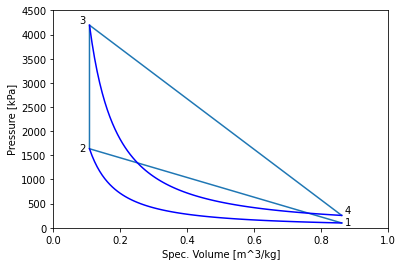
\includegraphics[width=0.6\textwidth]{secondPVDiagram}
%\captionof{figure}{}
%\label{fig:ch2_example1}
\end{center}

\subsubsection{Finishing Up}
To clean up the plot, we want to get rid of our original lines and manually put in the lines for constant volume heating and cooling.

For the first bit, we'll change our lines to simple circles by adding \verb~'ob'~ to the end of the plot command.  The \verb~o~ piece makes small circles instead of the lines, while \verb~b~ keeps the circles blue.

The command becomes:
\begin{Verbatim}[commandchars=\\\{\}]
plot([v1, v2, v3, v4], [p1, p2, p3, p4], \textcolor{purple}{'ob'})
\end{Verbatim}

In order to create the constant volume lines, we just connect the two points:
\begin{Verbatim}[commandchars=\\\{\}]
plot([v2, v3], [p2, p3], \textcolor{purple}{'b'})
plot([v4, v1], [p4, p1], \textcolor{purple}{'b'})
\end{Verbatim}

After all this, we end up with the final plot:
\begin{center}
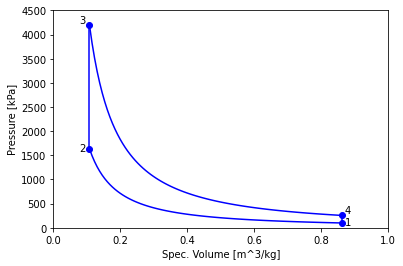
\includegraphics[width=0.6\textwidth]{finalPVDiagram}
%\captionof{figure}{}
%\label{fig:ch2_example1}
\end{center}

\subsubsection{Semi-log Plots}
There's an argument for using semi-log or log-log plots, depending on differences in pressure.

Replacing all of the \verb~plot~ commands with \verb~semilogy~ and changing the y-axis from a $0<p<4500$ to $50<p<5000$ yields the following plot:

\begin{center}
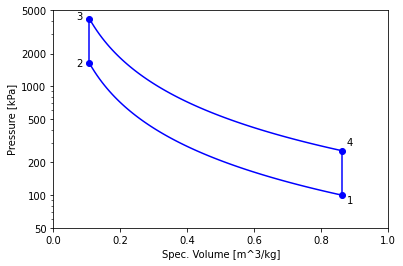
\includegraphics[width=0.6\textwidth]{finalPVDiagramSemilog}
%\captionof{figure}{}
%\label{fig:ch2_example1}
\end{center}

In order for the plot to come out well, it is also necessary to fiddle with the \verb~text~ commands.  In addition, to fix the tick labels on the $y$ axis, it is also necessary to add a \verb~yticks~ command:
\begin{Verbatim}[commandchars=\\\{\}]
yticks(ticks=[\textcolor{ForestGreen}{50}, \textcolor{ForestGreen}{100}, \textcolor{ForestGreen}{200}, \textcolor{ForestGreen}{500}, \textcolor{ForestGreen}{1000}, \textcolor{ForestGreen}{2000}, \textcolor{ForestGreen}{5000}], 
       labels=[\textcolor{ForestGreen}{50}, \textcolor{ForestGreen}{100}, \textcolor{ForestGreen}{200}, \textcolor{ForestGreen}{500}, \textcolor{ForestGreen}{1000}, \textcolor{ForestGreen}{2000}, \textcolor{ForestGreen}{5000}])
\end{Verbatim}

\section{Summary}
The main result from this chapter was the explanation of three engine cycles: Stirling, Otto, and Diesel.  Each of these cycles can convert excess heat, typically from combustion, to work.  The Stirling cycle can also use work in order to transfer heat from a cold environment to a hot environment, thus acting as either a heater or a refrigerator.  All of these cycles typically use ideal gases as the working fluid, so the ideal gas law was used in abundance.

In order to analyze these cycles, we introduced the First Law of Thermodynamics:
\begin{equation*}
  \Delta U = Q - W,
\end{equation*}
which is a statement of the conservation of energy.  The change in internal energy can be determined from the temperature change between states:
\begin{align*}
  \Delta U = U_2 - U_1 &= m c_v (T_2 - T_1) & \Delta u = u_2 - u_1 &= c_v (T_2 - T_1)
\end{align*}
The work is typically found through integration, which results in the following for special cases:
\begin{align*}
  {\rm Isobaric} & &\rightarrow& & W &= mp (v_2 - v_1) = p(V_2 - V_1)\\
  {\rm Isothermal} & &\rightarrow& & W &= mRT \ln \left(\frac{v_2}{v_1}\right)  = mRT \ln \left(\frac{V_2}{V_1}\right)\\
  {\rm Adiabatic} & &\rightarrow& & W &= m\:\frac{p_1 v_1 - p_2 v_2}{\gamma - 1} = m c_v (T_2-T_1)\\
  {\rm Isometric} & &\rightarrow& & W &= 0
\end{align*}

For the special case of constant pressure, the heat transfer for a process can be found using the constant pressure specific heat, $c_p$:

\begin{equation*}
  Q = m c_p (T_2 - T_1)
\end{equation*}

In all other circumstances, the heat transfer can only be determined through the First Law.

Finally, because two of the cycles use adiabatic compression/expansion, it was necessary to develop equations for the properties.  These are summarized below:

\begin{align*}
  \frac{p_2}{p_1} &= \left(\frac{T_2}{T_1}\right)^{\frac{\gamma}{\gamma -1}} = \left(\frac{v_1}{v_2}\right)^{\gamma} \\
  \frac{T_2}{T_1} &= \left(\frac{p_2}{p_1}\right)^{\frac{\gamma-1}{\gamma}} = \left(\frac{v_1}{v_2}\right)^{(\gamma -1)} \\
  \frac{v_2}{v_1} &= \left(\frac{p_1}{p_2}\right)^{\frac{1}{\gamma}} = \left(\frac{T_1}{T_2}\right)^{\frac{1}{(\gamma -1)}}
\end{align*}

\begin{homework}
  %{\bf Conceptual Questions}
  % Section 3.1 - First Law
  \question Look at Figure \ref{fig:ch3_pV}.  Which process would require the most work to complete?  What does this say about the heat transfer during that process?
  
  \question Why is work negative in the First Law of Thermodynamics?

  % Section 3.2 - Enthalpy
  \question In what circumstances is enthalpy useful?  In other words, why would we use enthalpy instead of internal energy?
  
  \question Which is larger, internal energy or enthalpy?  Is this always true?  Why?

  % Section 3.3 - Specific Heats
  \question In what ways is specific heat different between gases and solids?
  
  \question In words, what is $c_p$?

  % Section 3.4 - Stirling Cycle Engine
  \question What is the function of the regenerator?  Without a regenerator, what would be the effect on the engine?
  
  \question Is there heating that occurs during constant temperature expansion/compression?  If so, how much?
  
  % Section 3.5 - Stirling Cycle Cooling
  \question Draw the cycles in a $p$-$v$ diagram for the Stirling Cycle Engine and Stirling Cycle Cooler.  What is different between the two? Label all heat flow and work in and out of the the system.  Use $Q_H$, $Q_C$, $Q_R$, $W_{in}$, and $W_{out}$ for your labels.

  % Section 3.6 - Ideal Gas Adiabatic Processes
  \question What is $\gamma$?  How does it change with temperature (see Table \ref{sec:idealGasAir})?
  
  \question What assumptions are necessary to use Equations \ref{eq:ch3_adiabaticIdealGasTV}, \ref {eq:ch3_adiabaticIdealGaspV}, and \ref{eq:ch3_adiabaticIdealGaspT}?
  
  % Section 3.7 - Otto Cycle
  \question How does the Otto cycle differ from the Stirling cycle?
  
  \question What parameters determine the efficiency of the Otto cycle?
  
  % Section 3.8 - Diesel Cycle
  \question How does the Diesel cycle differ from the Stirling and Otto cycles?
  
  \question Why does the Diesel cycle typically use a higher compression ratio than the Otto cycle?


  % Work-out Questions
  %{\bf Work-out Questions}
  % Section 3.1 - 1st Law
  \question Four kilograms of water at 50°C are placed in a piston cylinder device under 6 MPa of pressure.  Heat is added to the water at constant pressure until the temperature of the steam reaches 400°C.
  \begin{questionparts}
  \item Determine the work done by the fluid ($W$) \answer{[1.1 kJ]} and the heat transferred to the fluid ($Q$) \answer{[11.9 kJ]} during this process. 
  \item Plot the process on a $p$-$v$ diagram.
  \end{questionparts}
  \newpage
  % Section 3.2 - Enthalpy
  \question For each of the following states, use the steam tables (or CoolProp) to check the relationship $h=u+pv$:
  \begin{questionparts}
  \item Steam at 300°C and a pressure of 200 kPa \\ \answer{[3072.1 kJ/kg = 2808.8 kJ/kg + 200 kPa $\cdot$ 1.3162 $\rm m^3/kg$]}
  \item R-134a at a specific volume of 1 $\rm m^3$/kg and an internal energy of 200 kJ/kg \answer{[206.5 kJ/kg]}
  \item Carbon dioxide at a temperature of -50°C and a pressure of 100 kPa (use CoolProp) \answer{[444.7 kJ/kg]}
  \item Helium at a temperature of -150°C and a pressure of 5 MPa (use CoolProp)\answer{[658.4 kJ/kg]}
  \end{questionparts}
  
  % Section 3.3 - Specific Heats
  \question How much heat is required to raise the temperature of Helium by 50°C at constant pressure? \answer{[259.7 kJ/kg]} What about at constant volume? \answer{[155.8 kJ/kg]}
  
  % Section 3.4 - Stirling Engine
  \question Analyze a Stirling cycle engine which uses air as a working fluid.  Let the minimum pressure be 400 kPa, the maximum volume be 1000 $\rm cm^3$, and the minimum volume be 400 $\rm cm^3$.  The temperature of the hot side is 100°C, and the temperature of the cold side is 20°C.
  \begin{questionparts}
  \item Sketch each process and state on a $p$-$v$ diagram.
  \item Find the pressure at each state. \answer{[$p_1 = 400 \rm kPa$, $p_2 = 1000 \rm kPa$, $p_3 = 1273 \rm kPa$, $p_4 = 509 \rm kPa$]}
  \item Create a table with the pressure, temperature, and specific volume at each state.
  \item Find the change of internal energy, work, and heat transfer for each process.  Put this information in a table.
  \item Find the net work of a cycle \answer{[100 J]}, the input heat transfer \answer{[466 J]}, and the thermal efficiency \answer{[21\%]}.
  \end{questionparts}
  \newpage
  %
  % Section 3.5 - Stirling Cooling
   \question Analyze a Stirling cycle cooler which uses helium as a working fluid.  Let the minimum pressure be 800 kPa, the maximum volume be 200 $\rm cm^3$, and the minimum volume be 150 $\rm cm^3$.  The temperature of the hot side is 20°C, and the temperature of the cold side is -30°C.
  \begin{questionparts}
  \item Sketch each process and state on a $p$-$v$ diagram.
  \item Find the pressure at each state. \answer{[$p_1 = 965 \rm kPa$, $p_2 = 1286 \rm kPa$, $p_3 = 1067 \rm kPa$, $p_4 = 800 \rm kPa$]}
  \item Create a table with the pressure, temperature, and specific volume at each state.
  \item Find the change of internal energy, work, and heat transfer for each process.  Put this information in a table.
  \item Find the net work per cycle \answer{[-9.5 J]}, the heat transfer from the refrigerated side \answer{[46 J]}, and the coefficient of performance \answer{[4.86]}.
  \end{questionparts}
  %
  % Section 3.6 - Ideal Gas Adiabatic Processes
  \question A frictionless piston-cylinder device contains 0.2 kg of air at 100 kPa and 27°C. The air is now compressed adiabatically until it reaches a final temperature of 77°C.

  \begin{questionparts}
  \item Sketch the P-V diagram of the process with respect to the relevant constant temperature lines, and indicate the work done on this diagram.
    
  \item Using the basic definition of boundary work done determine the boundary work done during the process \answer{[-7.18 kJ]}.
    
  \item Using the energy equation determine the heat transferred during the process \answer{[0 kJ]}, and verify that the process is in fact adiabatic.
  \end{questionparts}
  %
  Use values of specific heat capacity defined at 300K for the entire process.

  % Section 3.7 - Otto Cycle
  \question This is an extension of Example \ref{ex:ch3_otto}, in which we wish to use throughout all four processes the nominal standard specific heat capacity values for air at 300K. Using the values $c_v$ = 0.717 kJ/kgK and $\gamma$ = 1.4, determine:
  \begin{questionparts}
  \item the temperature and pressure of the air at the end of each process \answer{ [$p_2$ = 1838 kPa, $T_2$ = 689K, $T_3$ = 1805K, $p_3$ = 4815 kPa, $p_4$ = 262 kPa, $T_4$ = 786K] }

  \item  the net work output/cycle \answer{ [451.5 kJ/kg]}, and

  \item  the thermal efficiency of this engine cycle. \answer{ [$\eta_{th}$ = 56\%]}
  \end{questionparts}
  \newpage
  %
  % Section 3.8 - Diesel Cycle
  \question Consider the expansion stroke of a typical Air Standard Diesel cycle engine which has a compression ratio of 20 and a cutoff ratio of 2. At the beginning of the process (fuel injection) the initial temperature is 627°C, and the air expands at a constant pressure of 6.2 MPa until cutoff. Subsequently the air expands adiabatically (no heat transfer) until it reaches the maximum volume.
\begin{questionparts}
\item Sketch this process on a $p$-$v$ diagram showing clearly all three states. Shade on the diagram the total work done during the entire expansion process.
\item Determine the temperatures reached at the end of the constant pressure (fuel injection) process \answer{ [1800K]}, as well as at the end of the expansion process \answer{ [830K]}, and draw the three relevant constant temperature lines on the $p$-$v$ diagram.
\item Determine the total work done during the expansion stroke \answer{ [1087 kJ/kg]}.
\item Determine the total heat supplied to the air during the expansion stroke \answer{ [1028 kJ/kg]}.
\item Using Google Colab and CoolProp, plot the three states and two processes on a $p$-$v$ diagram.  Use the methodology in Section \ref{sec:plottingCurvedLines} to plot the curved expansion process.
\end{questionparts}
Use the specific heat values defined at 1000K for the entire expansion process, obtained from the table of Specific Heat Capacities of Air.

\question For an ideal Diesel engine with $r_c = 2$, what does the compression ratio need to be to match the efficiency of an ideal Otto engine with a compression ratio of $r=8$?

\end{homework}

